\documentclass[a4paper, 12pt, twoside]{ThesisStyle}
%\usepackage[utf8]{inputenc}
%%%%%%% anna defines

\usepackage{graphicx}
\usepackage{hyperref}
\usepackage{times}
\usepackage{textcomp}
\usepackage{latexsym}
\renewcommand{\UrlFont}{\ttfamily\small}
\usepackage{adjustbox}
\usepackage{latexsym}
\usepackage{amsmath}
\usepackage{subcaption}
\usepackage{verbatim}
\usepackage{balance}
\usepackage{graphicx}
\usepackage{amsmath}
\usepackage{subcaption}
\usepackage{array}
\usepackage[title]{appendix}
\usepackage{adjustbox}
\usepackage{multirow}
\usepackage{arydshln}
\usepackage{booktabs}
\usepackage{flushend}
\usepackage{enumitem}
\usepackage{tabularx}
\usepackage{natbib}
\usepackage{amssymb}
\setcitestyle{numbers,open={[},close={]},comma}
\setcounter{secnumdepth}{3} 
\newcommand{\paragraphHd}[1] {\vspace{3pt}\noindent\textbf{#1}}
\usepackage{mathtools}
\usepackage{etoolbox}
\appto\normalsize{\belowdisplayshortskip=\belowdisplayskip}
\usepackage{glossaries}

%%%%%%%%%%%%%%%%%%%%%%%%%%%%%%%%%%%%%%%%%%%%%%%%%%%%%

%%%%%%% template defines
\usepackage[hyphens]{url}
\usepackage{etex}
\usepackage{lmodern}
\usepackage[english]{babel}
\usepackage{floatrow}
\usepackage[dvipsnames]{xcolor}
\usepackage{amsmath,amssymb}             % AMS Math
% \usepackage[french]{babel}
\usepackage[utf8]{inputenc}
\usepackage[T1]{fontenc}
\usepackage[left=1.5in,right=1.3in,top=1.1in,bottom=1.1in,includefoot,includehead,headheight=13.6pt]{geometry}
\renewcommand{\baselinestretch}{1.05}

% Table of contents for each chapter

\usepackage[nottoc, notlof, notlot]{tocbibind}
\usepackage{minitoc}
\setcounter{minitocdepth}{2}
\mtcindent=15pt
% Use \minitoc where to put a table of contents


\usepackage{aecompl}


% Glossary / list of abbreviations

\usepackage[intoc]{nomencl}
\renewcommand{\nomname}{List of Abbreviations}

\makenomenclature

% My pdf code

\usepackage{ifpdf}

\usepackage{float}

\usepackage{subcaption}

\ifpdf
  \usepackage[pdftex]{graphicx}
%   \DeclareGraphicsExtensions{.jpg}
  \usepackage[a4paper,pagebackref,hyperindex=true]{hyperref}
  \usepackage[all]{hypcap}
  \usepackage{microtype}
\else
  \usepackage{graphicx}
%   \DeclareGraphicsExtensions{.ps,.eps}
  \usepackage[a4paper,dvipdfm,pagebackref,hyperindex=true]{hyperref}
  \usepackage[all]{hypcap}
  
% \usepackage{hypdvips}
% \usepackage{breakurl}
\fi

\graphicspath{{.}{images/}}

% Links in pdf
\usepackage{color}
\definecolor{linkcol}{rgb}{0.0,0.0,0.5} 
\definecolor{citecol}{rgb}{0.7,0,0} 
\definecolor{urlcol}{rgb}{0.0,0.5,0.0}

\definecolor{linkgray}{HTML}{54575e}
\definecolor{citationturquis}{HTML}{04b9b0}
\definecolor{referencebrown}{HTML}{57493e}

% Change this to change the informations included in the pdf file

% See hyperref documentation for information on those parameters

\hypersetup
{
bookmarksopen=true,
pdftitle="Extracting Personal Information from Conversations", 
pdfauthor="Anna Tigunova"
% pdfsubject="Creation of atlases and atlas based segmentation", %subject of the document
%pdftoolbar=false, % toolbar hidden
pdfmenubar=true, %menubar shown
pdfhighlight=/O, %effect of clicking on a link
colorlinks=true, %couleurs sur les liens hypertextes
% pdfpagemode=None, %aucun mode de page
pdfpagelayout=SinglePage, %ouverture en simple page
pdffitwindow=true, %pages ouvertes entierement dans toute la fenetre
%linkcolor=referencebrown,%MidnightBlue,%linkcol, %couleur des liens hypertextes internes
%citecolor=citationturquis,%BlueGreen, % citecol %couleur des liens pour les citations
%urlcolor=linkgray%LimeGreen, %urlcol %couleur des liens pour les url
}

% definitions.
% -------------------

\setcounter{secnumdepth}{3}
\setcounter{tocdepth}{2}

% Some useful commands and shortcut for maths:  partial derivative and stuff

\newcommand{\pd}[2]{\frac{\partial #1}{\partial #2}}
\def\abs{\operatorname{abs}}
\def\argmax{\operatornamewithlimits{arg\,max}}
\def\argmin{\operatornamewithlimits{arg\,min}}
\def\diag{\operatorname{Diag}}
\newcommand{\eqRef}[1]{(\ref{#1})}

\usepackage{rotating}%[figuresright]                   % Sideways of figures & tables
%\usepackage{bibunits}
%\usepackage[sectionbib]{chapterbib}          % Cross-reference package (Natural BiB)
%\usepackage{natbib}                  % Put References at the end of each chapter
                                         % Do not put 'sectionbib' option here.
                                         % Sectionbib option in 'natbib' will do.
\usepackage{fancyhdr}                    % Fancy Header and Footer

% \usepackage{txfonts}                     % Public Times New Roman text & math font
  
%%% Fancy Header %%%%%%%%%%%%%%%%%%%%%%%%%%%%%%%%%%%%%%%%%%%%%%%%%%%%%%%%%%%%%%%%%%
% Fancy Header Style Options

\pagestyle{fancy}                       % Sets fancy header and footer
\fancyfoot{}                            % Delete current footer settings


%\renewcommand{\chaptermark}[1]{         % Lower Case Chapter marker style
%  \markboth{\chaptername\ \thechapter.\ #1}}{}} %

%\renewcommand{\sectionmark}[1]{         % Lower case Section marker style
%  \markright{\thesection.\ #1}}         %

\fancyhead[LE,RO]{\bfseries\thepage}    % Page number (boldface) in left on even
% pages and right on odd pages
\fancyhead[RE]{\bfseries\nouppercase{\leftmark}}      % Chapter in the right on even pages
\fancyhead[LO]{\bfseries\nouppercase{\rightmark}}     % Section in the left on odd pages

\let\headruleORIG\headrule
\renewcommand{\headrule}{\color{black} \headruleORIG}
\renewcommand{\headrulewidth}{1.0pt}
\usepackage{colortbl}
\arrayrulecolor{black}

\fancypagestyle{plain}{
  \fancyhead{}
  \fancyfoot{}
  \renewcommand{\headrulewidth}{0pt}
}

\usepackage{algorithm}
\usepackage{algorithmic}

% \usepackage{algorithm}
% \usepackage[noend]{algorithmic}

\makeatletter
\def\theHALC...line{\thealgorithm-\theALC...line}
\def\theHALC...rem{\thealgorithm-\theALC...rem}
\makeatother

%%% Clear Header %%%%%%%%%%%%%%%%%%%%%%%%%%%%%%%%%%%%%%%%%%%%%%%%%%%%%%%%%%%%%%%%%%
% Clear Header Style on the Last Empty Odd pages
\makeatletter

\def\cleardoublepage{\clearpage\if@twoside \ifodd\c@page\else%
  \hbox{}%
  \thispagestyle{empty}%              % Empty header styles
  \newpage%
  \if@twocolumn\hbox{}\newpage\fi\fi\fi}

\makeatother
 
%%%%%%%%%%%%%%%%%%%%%%%%%%%%%%%%%%%%%%%%%%%%%%%%%%%%%%%%%%%%%%%%%%%%%%%%%%%%%%% 
% Prints your review date and 'Draft Version' (From Josullvn, CS, CMU)
\newcommand{\reviewtimetoday}[2]{\special{!userdict begin
    /bop-hook{gsave 20 710 translate 45 rotate 0.8 setgray
      /Times-Roman findfont 12 scalefont setfont 0 0   moveto (#1) show
      0 -12 moveto (#2) show grestore}def end}}
% You can turn on or off this option.
% \reviewtimetoday{\today}{Draft Version}
%%%%%%%%%%%%%%%%%%%%%%%%%%%%%%%%%%%%%%%%%%%%%%%%%%%%%%%%%%%%%%%%%%%%%%%%%%%%%%% 

\newenvironment{maxime}[1]
{
\vspace*{0cm}
\hfill
\begin{minipage}{0.5\textwidth}%
%\rule[0.5ex]{\textwidth}{0.1mm}\\%
\hrulefill $\:$ {\bf #1}\\
%\vspace*{-0.25cm}
\it 
}%
{%

\hrulefill
\vspace*{0.5cm}%
\end{minipage}
}

\let\minitocORIG\minitoc
\renewcommand{\minitoc}{\minitocORIG \vspace{1.5em}}

\usepackage{multirow}
% \usepackage{slashbox}

\newenvironment{bulletList}%
{ \begin{list}%
	{$\bullet$}%
	{\setlength{\labelwidth}{25pt}%
	 \setlength{\leftmargin}{30pt}%
	 \setlength{\itemsep}{\parsep}}}%
{ \end{list} }

% \newtheorem{definition}{Definition}
\renewcommand{\epsilon}{\varepsilon}

% centered page environment

\newenvironment{vcenterpage}
{\newpage\vspace*{\fill}\thispagestyle{empty}\renewcommand{\headrulewidth}{0pt}}
{\vspace*{\fill}}

% \usepackage[a4paper,pagebackref,hyperindex=true]{hyperref}
					% predefined styles
% \usepackage{graphicx}         % to use graphics
\usepackage{morefloats} 				% to allocate more floats
\usepackage{placeins}						% to flush floats within a section
\usepackage{tikz}								% to draw a graph
% \usepackage[utf8]{inputenc}			% UTF encoding
\usepackage{xspace}             % xspace - 'hard space'
% \usepackage{color}            % fonts coloring
\usepackage{amsthm}             % some useful things (such as proof environment)
\usepackage{amsfonts}           % some mathematical fonts
\usepackage{natbib}	% for the purpose of citations
% \usepackage[numbers]{natbib}
% \usepackage{subfig}							% for organizing images
\usepackage{lscape}							% to use landscape mode
\usepackage{bm}					% for bold symbols 
\usepackage{bbm}				% for dirac indicator
\usepackage{epsfig}
\usepackage{pgfplots}			
\usepackage{stmaryrd}			% for llbracket
\usepackage{eurosym} % defines \euro
\usepackage[mathletters]{ucs} % Extended unicode (utf-8) support
\usepackage{longtable} % longtable support required by pandoc >1.10
\usepackage{fancyvrb} % verbatim replacement that allows latex
\usepackage{grffile} % extends the file name processing of package graphics 
                         % to support a larger range 
\usepackage{booktabs}			% for better tables (like toprule)
\usepackage{makecell}			% for tabular
\usepackage[final]{pdfpages}
\usepackage{lettrine}
\usepackage{csquotes}
%%%%%%%%%%%%%%%%%%%%%%%%%%%%%%%%%%%%%%%%%%%%%%%%%%%

\addto\extrasenglish{%
	\renewcommand{\chapterautorefname}{Chapter}
	\renewcommand{\sectionautorefname}{Section}
	\renewcommand{\subsectionautorefname}{Section}
	\renewcommand{\subsubsectionautorefname}{Section}
}


%% 
% \newtheorem{definition}{Definition}[chapter]
% \newtheorem{fact}{Fact}
% \newtheorem{axiom}{Axiom}
% \newtheorem{theorem}{Theorem}[chapter]
% \newtheorem{lemma}{Lemma}[chapter]
% \newtheorem{corollary}{Corollary}[chapter]
% \newtheorem{example}{Example}
% \newcommand{\makeline}{\vspace{1mm}\hrule\vspace{1mm}}  % create a line
% \newcommand{\NOTE}[1]{\textcolor{red}{\\\textbf{Note: #1!}\\}}
% % \newenvironment{proof}{{\bf Proof\\}}{\\\hfill\rule[0.025cm]{0.21cm}{0.21cm}}
% 
% \newenvironment{notice}{\flushleft{\textbf{Notice:}}\\}
%   {\\\hfill\rule[0.025cm]{0.21cm}{0.21cm}}
% \newenvironment{examples}{\flushleft{\textbf{Examples:}}\begin{itemize}}
%   {\end{itemize}\hfill\rule[0.025cm]{0.21cm}{0.21cm}}%
% \newenvironment{solution}{\flushleft{\textbf{Solution:}}}
%   {\hfill\rule[0.025cm]{0.21cm}{0.21cm}}


% Some mathematical notations to simplify my life

% just to curiosity, not simplify my life too much
% \newcommand{\lonesurrogate}[1]{\ensuremath{|| #1 ||_{\epsilon}}}
% \newcommand{\lonesurrogateDefinition}[1]
% 	{\ensuremath{\lonesurrogate{#1} := \sum_j \sqrt{|#1_j|^2 + \epsilon} }}
\newcommand{\pnorm}[2]{\ensuremath{|| #1 ||_{#2}}}
\newcommand{\oneNorm}[1]{\pnorm{#1}{l_1}}
\newcommand{\twoNorm}[1]{\pnorm{#1}{l_2}}
\newcommand{\inftyNorm}[1]{\pnorm{#1}{l_{\infty}}}
\newcommand{\tvNorm}[1]{\pnorm{#1}{TV}}
\newcommand{\epsNorm}[1]{\ensuremath{|| #1 ||_{\epsilon}}}
\newcommand{\emptyNorm}[1]{\ensuremath{|| #1 ||}}
\newcommand{\orthoProjection}[1]{\ensuremath{{#1}{#1}^t}} 
\newcommand{\datafit}[1]{\ensuremath{||#1||^2_{l_2}}}   % data fit term
\newcommand{\pdatafit}[1]{\ensuremath{\frac{1}{2}||#1||^2_{l_2}}}
\newcommand{\sparsefit}[1]{\ensuremath{||#1||_{l_1}}}   % sparsity fit term
\newcommand{\relaxedfit}[1]{\ensuremath{(\epsilon + |#1|^2)^{1/2}}}
\newcommand{\drelaxedfit}[2]{#2^T (W^{-1} \otimes I_2) #2 #1}
\newcommand{\mtype}[3]{\mathbb{#1}^{#2 \times #3}}  % to write matrix type
\newcommand{\vtype}[2]{\mathbb{#1}^{#2}}
\newcommand{\set}[1]{\mathbb{#1}}
\newcommand{\setcal}[1]{\ensuremath{\mathcal{#1}}}
\newcommand{\bs}[1]{\ensuremath{\boldsymbol{#1}}}
\newcommand{\sgn}{\text{sgn}}
\newcommand{\diagonal}[1]{\ensuremath{\text{diag}\;#1}}
\newcommand{\half}{\ensuremath{\frac{1}{2}}}
\newcommand{\positiveProjection}[1]{\ensuremath{\left( #1 \right)_+}}
\newcommand{\setFormula}[2]{\ensuremath{
\left\{
#1 \; | \; #2
\right\} 
}}
\newcommand{\xstar}{\ensuremath{\bs{x}^{\star}}}
\newcommand{\ustar}{\ensuremath{\bs{u}^{\star}}}
\newcommand{\cSetSymbol}{\ensuremath{\setcal{C}}}
\newcommand{\cSetDefinition}{\ensuremath{\cSetSymbol := \vtype{R}{2}}}
\newcommand{\cSetSymbolHigherDimension}[1]{\ensuremath{\cSetSymbol{}^#1}}
\newcommand{\domain}[1]{\mbox{dom}(#1)}
\newcommand{\functionType}[2]{\ensuremath{  :  #1 \rightarrow #2}}
\newcommand{\extendedReals}{\ensuremath{{\set{\overline{R}}}}}
\newcommand{\best}[1]{\ensuremath{#1^{*}}}
\newcommand{\bestTwo}[2]{\ensuremath{#1^{*,#2}}}

% \DeclareMathOperator* {\argmin}{arg\, min}
% \DeclareMathOperator* {\argmax}{arg\, max}
\DeclareMathOperator* {\minimize}{minimize}
\DeclareMathOperator* {\maximize}{maximize}
\DeclareMathOperator* {\maximizeshort}{max.}
\DeclareMathOperator* {\equivunderscore}{\equiv}

%    \definecolor{orange}{cmyk}{0,0.4,0.8,0.2}
    \definecolor{darkorange}{rgb}{.71,0.21,0.01}
    \definecolor{darkgreen}{rgb}{.12,.54,.11}
    \definecolor{myteal}{rgb}{.26, .44, .56}
    \definecolor{gray}{gray}{0.45}
    \definecolor{lightgray}{gray}{.95}
    \definecolor{mediumgray}{gray}{.8}
    \definecolor{inputbackground}{rgb}{.95, .95, .85}
    \definecolor{outputbackground}{rgb}{.95, .95, .95}
    \definecolor{traceback}{rgb}{1, .95, .95}
    % ansi colors
    \definecolor{red}{rgb}{.6,0,0}
    \definecolor{green}{rgb}{0,.65,0}
    \definecolor{brown}{rgb}{0.6,0.6,0}
    \definecolor{blue}{rgb}{0,.145,.698}
    \definecolor{purple}{rgb}{.698,.145,.698}
    \definecolor{cyan}{rgb}{0,.698,.698}
    \definecolor{lightgray}{gray}{0.5}
    
    % bright ansi colors
    \definecolor{darkgray}{gray}{0.25}
    \definecolor{lightred}{rgb}{1.0,0.39,0.28}
    \definecolor{lightgreen}{rgb}{0.48,0.99,0.0}
    \definecolor{lightblue}{rgb}{0.53,0.81,0.92}
    \definecolor{lightpurple}{rgb}{0.87,0.63,0.87}
    \definecolor{lightcyan}{rgb}{0.5,1.0,0.83}
    
    % commands and environments needed by pandoc snippets
    % extracted from the output of `pandoc -s`
    \providecommand{\tightlist}{%
      \setlength{\itemsep}{0pt}\setlength{\parskip}{0pt}}
    \DefineVerbatimEnvironment{Highlighting}{Verbatim}{commandchars=\\\{\}}
    % Add ',fontsize=\small' for more characters per line
    \newenvironment{Shaded}{}{}
    \newcommand{\KeywordTok}[1]{\textcolor[rgb]{0.00,0.44,0.13}{\textbf{{#1}}}}
    \newcommand{\DataTypeTok}[1]{\textcolor[rgb]{0.56,0.13,0.00}{{#1}}}
    \newcommand{\DecValTok}[1]{\textcolor[rgb]{0.25,0.63,0.44}{{#1}}}
    \newcommand{\BaseNTok}[1]{\textcolor[rgb]{0.25,0.63,0.44}{{#1}}}
    \newcommand{\FloatTok}[1]{\textcolor[rgb]{0.25,0.63,0.44}{{#1}}}
    \newcommand{\CharTok}[1]{\textcolor[rgb]{0.25,0.44,0.63}{{#1}}}
    \newcommand{\StringTok}[1]{\textcolor[rgb]{0.25,0.44,0.63}{{#1}}}
    \newcommand{\CommentTok}[1]{\textcolor[rgb]{0.38,0.63,0.69}{\textit{{#1}}}}
    \newcommand{\OtherTok}[1]{\textcolor[rgb]{0.00,0.44,0.13}{{#1}}}
    \newcommand{\AlertTok}[1]{\textcolor[rgb]{1.00,0.00,0.00}{\textbf{{#1}}}}
    \newcommand{\FunctionTok}[1]{\textcolor[rgb]{0.02,0.16,0.49}{{#1}}}
    \newcommand{\RegionMarkerTok}[1]{{#1}}
    \newcommand{\ErrorTok}[1]{\textcolor[rgb]{1.00,0.00,0.00}{\textbf{{#1}}}}
    \newcommand{\NormalTok}[1]{{#1}}
    
    % Additional commands for more recent versions of Pandoc
    \newcommand{\ConstantTok}[1]{\textcolor[rgb]{0.53,0.00,0.00}{{#1}}}
    \newcommand{\SpecialCharTok}[1]{\textcolor[rgb]{0.25,0.44,0.63}{{#1}}}
    \newcommand{\VerbatimStringTok}[1]{\textcolor[rgb]{0.25,0.44,0.63}{{#1}}}
    \newcommand{\SpecialStringTok}[1]{\textcolor[rgb]{0.73,0.40,0.53}{{#1}}}
    \newcommand{\ImportTok}[1]{{#1}}
    \newcommand{\DocumentationTok}[1]{\textcolor[rgb]{0.73,0.13,0.13}{\textit{{#1}}}}
    \newcommand{\AnnotationTok}[1]{\textcolor[rgb]{0.38,0.63,0.69}{\textbf{\textit{{#1}}}}}
    \newcommand{\CommentVarTok}[1]{\textcolor[rgb]{0.38,0.63,0.69}{\textbf{\textit{{#1}}}}}
    \newcommand{\VariableTok}[1]{\textcolor[rgb]{0.10,0.09,0.49}{{#1}}}
    \newcommand{\ControlFlowTok}[1]{\textcolor[rgb]{0.00,0.44,0.13}{\textbf{{#1}}}}
    \newcommand{\OperatorTok}[1]{\textcolor[rgb]{0.40,0.40,0.40}{{#1}}}
    \newcommand{\BuiltInTok}[1]{{#1}}
    \newcommand{\ExtensionTok}[1]{{#1}}
    \newcommand{\PreprocessorTok}[1]{\textcolor[rgb]{0.74,0.48,0.00}{{#1}}}
    \newcommand{\AttributeTok}[1]{\textcolor[rgb]{0.49,0.56,0.16}{{#1}}}
    \newcommand{\InformationTok}[1]{\textcolor[rgb]{0.38,0.63,0.69}{\textbf{\textit{{#1}}}}}
    \newcommand{\WarningTok}[1]{\textcolor[rgb]{0.38,0.63,0.69}{\textbf{\textit{{#1}}}}}
    
    
    % Define a nice break command that doesn't care if a line doesn't already
    % exist.
    \def\br{\hspace*{\fill} \\* }
    % Math Jax compatability definitions
    \def\gt{>}
    \def\lt{<}
    % Document parameters
    \title{visual\_turing\_test}
    
    
    

    % Pygments definitions
    
\makeatletter
\def\PY@reset{\let\PY@it=\relax \let\PY@bf=\relax%
    \let\PY@ul=\relax \let\PY@tc=\relax%
    \let\PY@bc=\relax \let\PY@ff=\relax}
\def\PY@tok#1{\csname PY@tok@#1\endcsname}
\def\PY@toks#1+{\ifx\relax#1\empty\else%
    \PY@tok{#1}\expandafter\PY@toks\fi}
\def\PY@do#1{\PY@bc{\PY@tc{\PY@ul{%
    \PY@it{\PY@bf{\PY@ff{#1}}}}}}}
\def\PY#1#2{\PY@reset\PY@toks#1+\relax+\PY@do{#2}}

\expandafter\def\csname PY@tok@gd\endcsname{\def\PY@tc##1{\textcolor[rgb]{0.63,0.00,0.00}{##1}}}
\expandafter\def\csname PY@tok@gu\endcsname{\let\PY@bf=\textbf\def\PY@tc##1{\textcolor[rgb]{0.50,0.00,0.50}{##1}}}
\expandafter\def\csname PY@tok@gt\endcsname{\def\PY@tc##1{\textcolor[rgb]{0.00,0.27,0.87}{##1}}}
\expandafter\def\csname PY@tok@gs\endcsname{\let\PY@bf=\textbf}
\expandafter\def\csname PY@tok@gr\endcsname{\def\PY@tc##1{\textcolor[rgb]{1.00,0.00,0.00}{##1}}}
\expandafter\def\csname PY@tok@cm\endcsname{\let\PY@it=\textit\def\PY@tc##1{\textcolor[rgb]{0.25,0.50,0.50}{##1}}}
\expandafter\def\csname PY@tok@vg\endcsname{\def\PY@tc##1{\textcolor[rgb]{0.10,0.09,0.49}{##1}}}
\expandafter\def\csname PY@tok@vi\endcsname{\def\PY@tc##1{\textcolor[rgb]{0.10,0.09,0.49}{##1}}}
\expandafter\def\csname PY@tok@mh\endcsname{\def\PY@tc##1{\textcolor[rgb]{0.40,0.40,0.40}{##1}}}
\expandafter\def\csname PY@tok@cs\endcsname{\let\PY@it=\textit\def\PY@tc##1{\textcolor[rgb]{0.25,0.50,0.50}{##1}}}
\expandafter\def\csname PY@tok@ge\endcsname{\let\PY@it=\textit}
\expandafter\def\csname PY@tok@vc\endcsname{\def\PY@tc##1{\textcolor[rgb]{0.10,0.09,0.49}{##1}}}
\expandafter\def\csname PY@tok@il\endcsname{\def\PY@tc##1{\textcolor[rgb]{0.40,0.40,0.40}{##1}}}
\expandafter\def\csname PY@tok@go\endcsname{\def\PY@tc##1{\textcolor[rgb]{0.53,0.53,0.53}{##1}}}
\expandafter\def\csname PY@tok@cp\endcsname{\def\PY@tc##1{\textcolor[rgb]{0.74,0.48,0.00}{##1}}}
\expandafter\def\csname PY@tok@gi\endcsname{\def\PY@tc##1{\textcolor[rgb]{0.00,0.63,0.00}{##1}}}
\expandafter\def\csname PY@tok@gh\endcsname{\let\PY@bf=\textbf\def\PY@tc##1{\textcolor[rgb]{0.00,0.00,0.50}{##1}}}
\expandafter\def\csname PY@tok@ni\endcsname{\let\PY@bf=\textbf\def\PY@tc##1{\textcolor[rgb]{0.60,0.60,0.60}{##1}}}
\expandafter\def\csname PY@tok@nl\endcsname{\def\PY@tc##1{\textcolor[rgb]{0.63,0.63,0.00}{##1}}}
\expandafter\def\csname PY@tok@nn\endcsname{\let\PY@bf=\textbf\def\PY@tc##1{\textcolor[rgb]{0.00,0.00,1.00}{##1}}}
\expandafter\def\csname PY@tok@no\endcsname{\def\PY@tc##1{\textcolor[rgb]{0.53,0.00,0.00}{##1}}}
\expandafter\def\csname PY@tok@na\endcsname{\def\PY@tc##1{\textcolor[rgb]{0.49,0.56,0.16}{##1}}}
\expandafter\def\csname PY@tok@nb\endcsname{\def\PY@tc##1{\textcolor[rgb]{0.00,0.50,0.00}{##1}}}
\expandafter\def\csname PY@tok@nc\endcsname{\let\PY@bf=\textbf\def\PY@tc##1{\textcolor[rgb]{0.00,0.00,1.00}{##1}}}
\expandafter\def\csname PY@tok@nd\endcsname{\def\PY@tc##1{\textcolor[rgb]{0.67,0.13,1.00}{##1}}}
\expandafter\def\csname PY@tok@ne\endcsname{\let\PY@bf=\textbf\def\PY@tc##1{\textcolor[rgb]{0.82,0.25,0.23}{##1}}}
\expandafter\def\csname PY@tok@nf\endcsname{\def\PY@tc##1{\textcolor[rgb]{0.00,0.00,1.00}{##1}}}
\expandafter\def\csname PY@tok@si\endcsname{\let\PY@bf=\textbf\def\PY@tc##1{\textcolor[rgb]{0.73,0.40,0.53}{##1}}}
\expandafter\def\csname PY@tok@s2\endcsname{\def\PY@tc##1{\textcolor[rgb]{0.73,0.13,0.13}{##1}}}
\expandafter\def\csname PY@tok@nt\endcsname{\let\PY@bf=\textbf\def\PY@tc##1{\textcolor[rgb]{0.00,0.50,0.00}{##1}}}
\expandafter\def\csname PY@tok@nv\endcsname{\def\PY@tc##1{\textcolor[rgb]{0.10,0.09,0.49}{##1}}}
\expandafter\def\csname PY@tok@s1\endcsname{\def\PY@tc##1{\textcolor[rgb]{0.73,0.13,0.13}{##1}}}
\expandafter\def\csname PY@tok@ch\endcsname{\let\PY@it=\textit\def\PY@tc##1{\textcolor[rgb]{0.25,0.50,0.50}{##1}}}
\expandafter\def\csname PY@tok@m\endcsname{\def\PY@tc##1{\textcolor[rgb]{0.40,0.40,0.40}{##1}}}
\expandafter\def\csname PY@tok@gp\endcsname{\let\PY@bf=\textbf\def\PY@tc##1{\textcolor[rgb]{0.00,0.00,0.50}{##1}}}
\expandafter\def\csname PY@tok@sh\endcsname{\def\PY@tc##1{\textcolor[rgb]{0.73,0.13,0.13}{##1}}}
\expandafter\def\csname PY@tok@ow\endcsname{\let\PY@bf=\textbf\def\PY@tc##1{\textcolor[rgb]{0.67,0.13,1.00}{##1}}}
\expandafter\def\csname PY@tok@sx\endcsname{\def\PY@tc##1{\textcolor[rgb]{0.00,0.50,0.00}{##1}}}
\expandafter\def\csname PY@tok@bp\endcsname{\def\PY@tc##1{\textcolor[rgb]{0.00,0.50,0.00}{##1}}}
\expandafter\def\csname PY@tok@c1\endcsname{\let\PY@it=\textit\def\PY@tc##1{\textcolor[rgb]{0.25,0.50,0.50}{##1}}}
\expandafter\def\csname PY@tok@o\endcsname{\def\PY@tc##1{\textcolor[rgb]{0.40,0.40,0.40}{##1}}}
\expandafter\def\csname PY@tok@kc\endcsname{\let\PY@bf=\textbf\def\PY@tc##1{\textcolor[rgb]{0.00,0.50,0.00}{##1}}}
\expandafter\def\csname PY@tok@c\endcsname{\let\PY@it=\textit\def\PY@tc##1{\textcolor[rgb]{0.25,0.50,0.50}{##1}}}
\expandafter\def\csname PY@tok@mf\endcsname{\def\PY@tc##1{\textcolor[rgb]{0.40,0.40,0.40}{##1}}}
\expandafter\def\csname PY@tok@err\endcsname{\def\PY@bc##1{\setlength{\fboxsep}{0pt}\fcolorbox[rgb]{1.00,0.00,0.00}{1,1,1}{\strut ##1}}}
\expandafter\def\csname PY@tok@mb\endcsname{\def\PY@tc##1{\textcolor[rgb]{0.40,0.40,0.40}{##1}}}
\expandafter\def\csname PY@tok@ss\endcsname{\def\PY@tc##1{\textcolor[rgb]{0.10,0.09,0.49}{##1}}}
\expandafter\def\csname PY@tok@sr\endcsname{\def\PY@tc##1{\textcolor[rgb]{0.73,0.40,0.53}{##1}}}
\expandafter\def\csname PY@tok@mo\endcsname{\def\PY@tc##1{\textcolor[rgb]{0.40,0.40,0.40}{##1}}}
\expandafter\def\csname PY@tok@kd\endcsname{\let\PY@bf=\textbf\def\PY@tc##1{\textcolor[rgb]{0.00,0.50,0.00}{##1}}}
\expandafter\def\csname PY@tok@mi\endcsname{\def\PY@tc##1{\textcolor[rgb]{0.40,0.40,0.40}{##1}}}
\expandafter\def\csname PY@tok@kn\endcsname{\let\PY@bf=\textbf\def\PY@tc##1{\textcolor[rgb]{0.00,0.50,0.00}{##1}}}
\expandafter\def\csname PY@tok@cpf\endcsname{\let\PY@it=\textit\def\PY@tc##1{\textcolor[rgb]{0.25,0.50,0.50}{##1}}}
\expandafter\def\csname PY@tok@kr\endcsname{\let\PY@bf=\textbf\def\PY@tc##1{\textcolor[rgb]{0.00,0.50,0.00}{##1}}}
\expandafter\def\csname PY@tok@s\endcsname{\def\PY@tc##1{\textcolor[rgb]{0.73,0.13,0.13}{##1}}}
\expandafter\def\csname PY@tok@kp\endcsname{\def\PY@tc##1{\textcolor[rgb]{0.00,0.50,0.00}{##1}}}
\expandafter\def\csname PY@tok@w\endcsname{\def\PY@tc##1{\textcolor[rgb]{0.73,0.73,0.73}{##1}}}
\expandafter\def\csname PY@tok@kt\endcsname{\def\PY@tc##1{\textcolor[rgb]{0.69,0.00,0.25}{##1}}}
\expandafter\def\csname PY@tok@sc\endcsname{\def\PY@tc##1{\textcolor[rgb]{0.73,0.13,0.13}{##1}}}
\expandafter\def\csname PY@tok@sb\endcsname{\def\PY@tc##1{\textcolor[rgb]{0.73,0.13,0.13}{##1}}}
\expandafter\def\csname PY@tok@k\endcsname{\let\PY@bf=\textbf\def\PY@tc##1{\textcolor[rgb]{0.00,0.50,0.00}{##1}}}
\expandafter\def\csname PY@tok@se\endcsname{\let\PY@bf=\textbf\def\PY@tc##1{\textcolor[rgb]{0.73,0.40,0.13}{##1}}}
\expandafter\def\csname PY@tok@sd\endcsname{\let\PY@it=\textit\def\PY@tc##1{\textcolor[rgb]{0.73,0.13,0.13}{##1}}}

\def\PYZbs{\char`\\}
\def\PYZus{\char`\_}
\def\PYZob{\char`\{}
\def\PYZcb{\char`\}}
\def\PYZca{\char`\^}
\def\PYZam{\char`\&}
\def\PYZlt{\char`\<}
\def\PYZgt{\char`\>}
\def\PYZsh{\char`\#}
\def\PYZpc{\char`\%}
\def\PYZdl{\char`\$}
\def\PYZhy{\char`\-}
\def\PYZsq{\char`\'}
\def\PYZdq{\char`\"}
\def\PYZti{\char`\~}
% for compatibility with earlier versions
\def\PYZat{@}
\def\PYZlb{[}
\def\PYZrb{]}
\makeatother


    % Exact colors from NB
    \definecolor{incolor}{rgb}{0.0, 0.0, 0.5}
    \definecolor{outcolor}{rgb}{0.545, 0.0, 0.0}


    % Slightly bigger margins than the latex defaults
    
    % \geometry{verbose,tmargin=3cm,bmargin=3.2cm,lmargin=2.5cm,rmargin=2.5cm}
    

%\newcommand{\scream}[1]{\textbf{*** #1! ***}}
% useful abbreviations
 \newcommand{\fixme}[1]{\textcolor{red}{\textbf{FiXme}#1}\xspace}
 \newcommand{\hobs}{\textrm{h}_\textrm{obs}}
 \newcommand{\cpad}[1]{@{\hspace{#1mm}}}
 \newcommand{\alg}[1]{\textsc{#1}}

 \newcommand{\fnrot}[2]{\scriptsize\rotatebox{90}{\begin{minipage}{#1}\flushleft #2\end{minipage}}}
 \newcommand{\chmrk}{{\centering\ding{51}}}
 \newcommand{\eqn}[1]{\begin{eqnarray}\vspace{-1mm}#1\vspace{-1mm}\end{eqnarray}}
 \newcommand{\eqns}[1]{\begin{eqnarray*}\vspace{-1mm}#1\vspace{-1mm}\end{eqnarray*}}
 
 
\newcommand{\todo}[1]{\textcolor{DarkOrchid}{ToDo: #1}}
%\newcommand{\myparagraph}[1]{\vspace{-0.25cm} \paragraph{#1}}
\newcommand{\myparagraph}[1]{\paragraph{#1}}

\newcommand{\invisible}[1]{\emph{#1}}%{}

\newcommand{\figvspace}{\vspace{-.5cm}}
\newcommand{\secvspace}{\vspace{-.2cm}}
\newcommand{\subsecvspace}{\vspace{-.2cm}}

\graphicspath{{./fig/}{./fig/plots/}}


\newcommand{\iccvArch}{Ask Your Neurons\xspace}
\newcommand{\newArch}{Refined Ask Your Neurons\xspace}

\newcommand{\AproachName}{Ask Your Neurons\xspace}
\newcommand{\daquarNew}{DAQUAR-Consensus\xspace}
\newcommand{\visualturingtest}{Visual Turing Test\xspace}

\newcommand{\factnet}{Visual~FactNet\xspace}


\newcommand*{\droppedcapital}[2]{\lettrine[lines=3]{\textcolor{Emerald}#1}{#2}}

\newcommand{\qenc}[1]{\Psi_{\text{#1}}(\bs{q})}
\newcommand{\ienc}{\Phi(\bs{x})\xspace}

% for cross-reference footnotes
\newcommand{\footlabel}[2]{%
    \addtocounter{footnote}{1}%
    \footnotetext[\thefootnote]{%
        \addtocounter{footnote}{-1}%
        \refstepcounter{footnote}\label{#1}%
        #2%
    }%
    $^{\ref{#1}}$%
}

\newcommand{\footref}[1]{%
    $^{\ref{#1}}$%
}

%

 % cvpr crap
 %\usepackage[pagebackref=true,breaklinks=true,letterpaper=true,colorlinks,bookmarks=false]{hyperref}
 \def\httilde{\mbox{\tt\raisebox{-.5ex}{\symbol{126}}}}

 % Add a period to the end of an abbreviation unless there's one
 \makeatletter
 \DeclareRobustCommand\onedot{\futurelet\@let@token\@onedot}
 \def\@onedot{\ifx\@let@token.\else.\null\fi\xspace}
 \def\eg{e.g\onedot} \def\Eg{E.g\onedot}
 \def\ie{i.e\onedot} \def\Ie{I.e\onedot}
 \def\cf{cf\onedot} \def\Cf{Cf\onedot}
 \def\etc{etc\onedot} \def\vs{vs\onedot}
 \def\wrt{w.r.t\onedot} \def\dof{d.o.f\onedot}
 \def\etal{\textit{et~al\onedot}} \def\iid{i.i.d\onedot}
 \def\Fig{Fig\onedot} \def\Eqn{Eqn\onedot} \def\Sec{Sec\onedot}
 \def\vs{vs\onedot}
 \makeatother

% to conform Springer (do not change it!)
\DeclareRobustCommand{\figref}[1]{Figure~\ref{#1}}
\DeclareRobustCommand{\figsref}[1]{Figures~\ref{#1}}

\DeclareRobustCommand{\Figref}[1]{Figure~\ref{#1}}
\DeclareRobustCommand{\Figsref}[1]{Figures~\ref{#1}}

\DeclareRobustCommand{\Secref}[1]{Section~\ref{#1}}
\DeclareRobustCommand{\secref}[1]{Section~\ref{#1}}

\DeclareRobustCommand{\Secsref}[1]{Sections~\ref{#1}}
\DeclareRobustCommand{\secsref}[1]{Sections~\ref{#1}}

\DeclareRobustCommand{\Tableref}[1]{Table~\ref{#1}}
\DeclareRobustCommand{\tableref}[1]{Table~\ref{#1}}

\DeclareRobustCommand{\Tablesref}[1]{Tables~\ref{#1}}
\DeclareRobustCommand{\tablesref}[1]{Tables~\ref{#1}}

\DeclareRobustCommand{\eqnref}[1]{Equation~(\ref{#1})}
\DeclareRobustCommand{\Eqnref}[1]{Equation~(\ref{#1})}

\DeclareRobustCommand{\eqnsref}[1]{Equations~(\ref{#1})}
\DeclareRobustCommand{\Eqnsref}[1]{Equations~(\ref{#1})}

\DeclareRobustCommand{\chapref}[1]{Chapter~\ref{#1}}
\DeclareRobustCommand{\Chapref}[1]{Chapter~\ref{#1}}

\DeclareRobustCommand{\chapsref}[1]{Chapters~\ref{#1}}
\DeclareRobustCommand{\Chapsref}[1]{Chapters~\ref{#1}}


 % itemize without all the whitespace
%  \newenvironment{itemize1}{
%  \begin{itemize}
%    \setlength{\itemsep}{1pt}
%    \setlength{\parskip}{0pt}
%    \setlength{\parsep}{0pt}
%  }{\end{itemize}}
% 
 

% \setlength{\topskip}{0mm}
 \setlength{\abovecaptionskip}{3mm}
 \setlength{\belowcaptionskip}{3mm}
 \setlength{\textfloatsep}{5mm}


\DeclareMathOperator{\avg}{avg}

\newcommand{\squishlist}{
   \begin{list}{$\bullet$}
    { \setlength{\itemsep}{0pt}      \setlength{\parsep}{3pt}
      \setlength{\topsep}{3pt}       \setlength{\partopsep}{0pt}
      \setlength{\leftmargin}{1.5em} \setlength{\labelwidth}{1em}
      \setlength{\labelsep}{0.5em} } }
\newcommand{\squishlisttwo}{
   \begin{list}{$\bullet$}c% \settopmatter{printacmref=false} % Removes citation information below abstract
% \renewcommand\footnotetextcopyrightpermission[1]{} % removes footnote with conference information in first column
% \pagestyle{plain} % removes running headers
    { \setlength{\itemsep}{0pt}    \setlength{\parsep}{0pt}
      \setlength{\topsep}{0pt}     \setlength{\partopsep}{0pt}
      \setlength{\leftmargin}{0.9em} \setlength{\labelwidth}{0.5em}
      \setlength{\labelsep}{0.5em} } }

\newcommand{\squishend}{
    \end{list} 
}

\newtheorem{defn}{Definition}
\newtheorem{prop}{Proposition}
\newtheorem{corol}{Corollary}

%tfidf+variants
\newcommand{\bowVanilla}{\textsc{bow}}
\newcommand{\bowD}{\textsc{bow-d}}
\newcommand{\bowT}{\textsc{bow-t}}
\newcommand{\bowDT}{\textsc{bow-dt}}

%lda+variants
\newcommand{\ldaVanilla}{\textsc{lda}}
\newcommand{\ldaD}{\textsc{lda-d}}
\newcommand{\ldaT}{\textsc{lda-t}}
\newcommand{\ldaDT}{\textsc{lda-dt}}

%w2v+variants
\newcommand{\wtovVanilla}{\textsc{w2v}}
\newcommand{\wtovD}{\textsc{w2v-d}}
\newcommand{\wtovT}{\textsc{w2v-t}}
\newcommand{\wtovDT}{\textsc{w2v-dt}}

\newcounter{qcounter}
\newenvironment{questions}{
 \begin{list}{\textbf{RQ \arabic{qcounter}:}~}{\usecounter{qcounter}}
}{
 \end{list}
}


\newcommand*{\droppedcapital}[2]{\lettrine[lines=3]{\textcolor{Emerald}#1}{#2}}

\newcommand{\method}[1]{HAM$_{\text{\,#1}}$}
\newcommand{\charm}[1]{CHARM$_{\text{\,#1}}$}
\newcommand{\wiki}[1]{Wiki-#1}
\newcommand{\attribute}[1]{\textbf{\emph{#1}}}
\newcommand{\paragraphHdTop}[1] {\noindent\textbf{#1}} % use for first in a series of paragraphHd's

\newcommand{\squishlist}{
 \begin{list}{$\bullet$}
  { \setlength{\itemsep}{7pt}
     \setlength{\parsep}{1pt}
     \setlength{\topsep}{4pt}
     \setlength{\partopsep}{0pt}
     \setlength{\leftmargin}{1.5em}
     \setlength{\labelwidth}{1em}
     \setlength{\labelsep}{0.5em} } }

\newcommand{\squishend}{
  \end{list}  }
  
\newcommand{\sig}[1]{#1*}
\newcommand{\nsig}[1]{#1\phantom{*}}
\newcommand{\bsig}[1]{\textbf{#1}*}
\newcommand{\bnsig}[1]{\textbf{#1}\phantom{*}}
\newcommand{\best}[1]{\textbf{#1}}

\usepackage{hyphenat}
\hyphenation{spea-ker}
\hyphenation{lib-ra-ry}


\newcommand\myshade{85}
\colorlet{mylinkcolor}{YellowOrange}
\colorlet{mycitecolor}{Aquamarine}
\colorlet{myurlcolor}{Blue}

% Prevent overflowing lines due to hard-to-break entities
%\sloppy 
% Setup hyperref package
\let\oldciteauthor=\citeauthor
\def\citeauthor#1{\hypersetup{citecolor=black}\oldciteauthor{#1}}
\let\oldcite=\cite
\def\cite#1{\hypersetup{citecolor=mycitecolor}\oldcite{#1}}
\let\oldcitet=\citet
\def\citet#1{\hypersetup{citecolor=mycitecolor}\oldcitet{#1}}
 \hypersetup{
       breaklinks=true,  % so long urls are correctly broken across lines
       colorlinks=true,
       urlcolor=myurlcolor,
       linkcolor=mylinkcolor,
       citecolor=mycitecolor,
       }


\newfloatcommand{capbtabbox}{table}[][\FBwidth]
\newcommand*\rot{\rotatebox{90}}
%% Bibliography Setting
%\bibliographystyle{abbrvnat}
% \bibliographystyle{MinThesisStyle}
\bibliographystyle{plainnat}
\setcitestyle{square,aysep={}}

% don't put more spacing at the end of the line
\frenchspacing

% set spacing between lines
\linespread{1.21}
\selectfont
% \onehalfspacing
% \doublespacing
% \setstretch{1.08}


% if this thesis is a draft it should be written '(Draft)'; otherwise null
\newcommand{\isDraft}{(Draft)}
%\newcommand{\isDraft}{}

\setlength{\headheight}{24pt}

\makeglossaries

\newglossaryentry{PyTorch}
{
    name=PyTorch,
    description={https://pytorch.org}
}

\newglossaryentry{Scikit-learn}
{
    name=Scikit-learn,
    description={https://scikit-learn.org}
}

\newglossaryentry{word2vec}
{
    name=word2vec,
    description={https://code.google.com/archive/p/word2vec}
}

\newglossaryentry{GloVe}
{
    name=GloVe,
    description={https://nlp.stanford.edu/projects/glove}
}

\newglossaryentry{Cornell Movie-Dialogs Corpus}
{
    name=Cornell Movie-Dialogs Corpus,
    description={https://www.cs.cornell.edu/~cristian/Cornell_Movie-Dialogs_Corpus.html}
}

\newglossaryentry{MTurk}
{
    name=MTurk,
    description={https://www.mturk.com}
}

\newglossaryentry{IMDb}
{
    name=IMDb,
    description={https://www.imdb.com}
}

\newglossaryentry{GradeSaver}
{
    name=GradeSaver,
    description={https://www.gradesaver.com}
}

\newglossaryentry{Crowdsourcing comparison tool by Zheng et al.}
{
    name= ,
    description={https://zhydhkcws.github.io/crowd_truth_inference/index.html}
}

\newglossaryentry{IMSDb}
{
    name=IMSDb,
    description={https://imsdb.com}
}

\newglossaryentry{Reddit dump}
{
    name=Reddit dump,
    description={https://files.pushshift.io/reddit}
}

\newglossaryentry{Snorkel framework}
{
    name=Snorkel framework,
    description={https://www.snorkel.org}
}

\newglossaryentry{PersonaChat corpus}
{
    name=PersonaChat corpus,
    description={http://convai.io/\#personachat-convai2-dataset}
}

\newglossaryentry{ELMo model}
{
    name=ELMo model,
    description={https://allennlp.org/elmo}
}

\newglossaryentry{BERT}
{
    name=BERT,
    description={https://huggingface.co/transformers/model_doc/bert.html}
}

\newglossaryentry{TREC Web Track}
{
    name=TREC Web Track,
    description={https://trec.nist.gov/data/webmain.html}
}

\newglossaryentry{RAKE}
{
    name=RAKE,
    description={https://pypi.org/project/rake-nltk}
}

\newglossaryentry{TextRank}
{
    name=TextRank,
    description={https://pypi.org/project/pytextrank}
}

\newglossaryentry{Flask}
{
    name=Flask,
    description={https://flask.palletsprojects.com}
}
\newcolumntype{A}{>{\centering}p{0.25\textwidth}}
\newcolumntype{B}{>{\centering\arraybackslash}p{0.25\textwidth}}

% #-------------------------------------------------------------------------# 
\begin{document}

%% Proper document
\pagenumbering{roman}

% It needs \usepackage{epsfig}

\frontmatter%
\begin{titlepage}

\def\docdate{2018}

\newlength{\longskip}
\setlength{\longskip}{0.03\textheight}

\rmfamily
\vspace*{\stretch{0.5}}

\begin{center}

\hrulefill\par
\huge{
    \vspace{0.5cm}
 \textbf{Enhancing Privacy and Fairness \\in Search Systems} \\
      }
\hrulefill\par
\vspace*{\stretch{1.7}}

% \Large
% A dissertation submitted towards the degree  \\
% Doctor of Engineering Science \\
% (Dr.-Ing.)\\
% of the Faculty of Mathematics and Computer Science\\ 
% of Saarland University
% \vspace*{\stretch{1}}


\Large
% Dissertation zur Erlangung des Grades \\
% Doktor der Ingenieurwissenschaften (Dr.-Ing.) \\
% der Naturwissenschaftlich-Technischen Fakult\"{a}ten \\
% der Universit\"{a}t des Saarlandes
A dissertation submitted towards the degree \\
Doctor of Engineering (Dr.-Ing.) \\
of the Faculty of Mathematics and Computer Science \\
of Saarland University
\vspace*{\stretch{1}}


%by \\%[\longskip]
by \\
\textbf{JOANNA BIEGA}%, M.Sc. 
%\\ (aka Asia J. Biega)} \\[1em]
% {\large \ in Informatik} \\
% {\large born in Frankfurt am Main, Germany} \\
%born 22${}^{\mathsf{nd}}$ \hspace*{-0.55mm}of November, 1978 \\
%in Mainz, Germany\vspace*{\stretch{1}}

% Prof.\ Dr.-Ing.\ Bernt Schiele, examiner \\
% Prof.\ Dr.\ Manfred Pinkal, co-examiner 
% \vspace*{\stretch{1}}


% Date of Defense: 10${}^{\mathsf{th}}$ \hspace*{-0.55mm}of February, 2013

\vspace*{\stretch{1}}

Saarbr\"ucken\\ 
December 2018
\end{center}


% \vspace*{-2.0cm}\hspace*{-2.00cm}%
% \parbox{5.0cm}{\epsfig{file=figures/mpi_logo/mpilogo-inf-compact, width=4.5cm}}%\hfill%
% \parbox[][2.5cm][c]{7.8cm}{%
% \begin{center}
%   Universit\"at des Saarlandes \\
%   Faculty of Natural Science and Technology I \\
%   Computer Science
% \end{center}
% }%\hfill%
% \hspace{0.5cm}
% \parbox{5.0cm}{\epsfig{file=figures/mmci_uds_logo/UdS_Logo_NEU, width=5.0cm}}
% % \parbox{5.5cm}{\epsfig{file=figures/mpi_logo/mpilogo-inf-compact, width=4.5cm}}
% % \hspace{0.03cm}
% % \parbox{7.5cm}{\epsfig{file=figures/mpi_logo/imprs_logo, width=6.5cm}}
% % \\[0.1cm]
% % \begin{center}
% %   School of Computer and Communication Sciences, \\
% %   Ecole Polytechnique Federale de Lausanne, Switzerland
% % \end{center}
% % \hspace{0.5cm}
% \\[2.0cm]
%
% \begin{center}
% % \textbf{\Huge %\hspace{1.5cm}%
% % Ask Your Neurons: \\
% % From Object Recognition \\[0.25cm]
% % Towards Visual Turing Test} \\[3.5cm]
% {\Huge\textbf{ %\hspace{1.5cm}
% Towards Holistic Machines:} \\[0.1cm]
% From Visual Recognition \\
% To Question Answering \\[0.5cm]
% About Real-World Images} \\[4.0cm]
% %\hspace{1.5cm}
% Thesis for obtaining the degree\\
% %\hspace{1.5cm}
% {\Large
% Doctor of Engineering \\
% (Dr.-Ing.) \\[0.3cm]}
% %\hspace{1.5cm}
% by\\[0.3cm]
% \textbf{\Large %\hspace{1.5cm}
% Mateusz Malinowski, M.Sc.}\\[1.5cm]
% \end{center}
%
% \begin{center}\large
% \vspace{2.8cm}
% Saarbr\"ucken \\
% \today
% \end{center}
\end{titlepage}



\dominitoc

% \cleardoublepage

%
% diplom/thesis/frontmatter.tex -- dedication, abstract, etc.
% $Id$
%

% \section*{}
% \vspace*{2.0cm}
% \textbf{Non-plagiarism Statement}
% I hereby confirm that this thesis is my own work and that I have documented all
% sources used.
%
% \vspace{1.5cm} \noindent
% (Mateusz Malinowski) \\
% Saarbr\"{u}cken, \today
% \vspace{2.5cm}
%
% \noindent \textbf{Declaration of Consent}
% I herewith agree that my thesis will be made available through the library of
% the Computer Science Department.
%
% \vspace{1.5cm}
% \noindent (Mateusz Malinowski) \\
% Saarbr\"{u}cken, \today

\newpage
\noindent
\textbf{Defense Colloquium} \\[0.25cm]
Date: \hspace{3.2cm}1 April 2019\\[1cm]
Dean of the Faculty: \hspace{0.88cm}Prof. Dr. Sebastian Hack \\[2.5cm]
% \hspace*{4.05cm} Saarland University, Germany \\[2.5cm]
%
\textbf{Examination Committee} \\[0.25cm]
Chair: \hspace{3.1cm}Prof. Dr. Bernt Schiele\\[1.0cm]%Prof. XYZ\\[1.0cm]
% \hspace*{4.05cm}Saarland University, Germany \\[1.0cm]
%
Reviewer, Advisor: \hspace{1.05cm} Prof. Dr. Gerhard Weikum\\[1.0cm]
% \hspace*{4.05cm}Max Planck Institute for Informatics, Germany \\[1.0cm]
%
Reviewer, Co-Advisor: \hspace{0.55cm} Prof. Dr. Krishna P. Gummadi\\[1.0cm]
% \hspace*{4.05cm}Max Planck Institute for Software Systems, Germany \\[1.0cm]
%
Reviewer: \hspace{2.50cm} Prof. Dr. Carlos Castillo\\[1.0cm]
% \hspace*{4.05cm}University of \\[1.0cm]
%
Reviewer: \hspace{2.50cm} Prof. Dr. Wolfgang Nejdl\\[1.0cm]
% \hspace*{4.05cm}University of \\[1.0cm]
%
Academic Assistant: \hspace{0.92cm} Dr. Erisa Terolli\\[1.0cm]%Dr. XYZ\\[1.0cm]
% \hspace*{4.05cm}Max Planck Institute for Informatics, Germany\\[1.0cm]

\cleardoublepage

%% Here should be the acknowledgements
%\input{Acknowledgements}

\cleardoublepage

\input{Abstract}




\tableofcontents

\cleardoublepage

\mainmatter

\chapter{Introduction}
\minitoc
\section{Motivation and Problem Statement}
\label{mot}

\droppedcapital{T}HE recent rise of social media enabled the access to vast amounts of user-generated content. This data has many potential applications; \textit{personalization} being a major use case.

Having background information about the user is practical for many downstream applications, such as recommender systems and search engines \cite{balog2019personal}. 
For instance, the ranking results for the query ``best weekend activities in Vancouver'' can be rearranged based on the user's known hobbies to deliver more topical content for a particular individual. Another application greatly benefiting from the availability of the user's background is personalized intelligent assistants.

Chat-bots have become an essential part of everyday life, being able to deal with a wide range of routine tasks, provide factual information and entertain the user. Still, there is a growing demand for creating user-oriented intelligent agents, which are able to hold personalized conversations, while at the same time building and expanding their knowledge repository about the user's traits and preferences. 

Having access to the user's interests and background, personalized chat-bots will be able to build relevant responses and start new topics, interesting for the user. The ability to produce meaningful or even funny and surprising utterances is a desired feature, making a chat-bot appealing to the user. Therefore, there has been significant research interest in personalizing intelligent assistants, which still remains challenging. 

Consider, for example, the following conversation between a human (H) and an intelligent assistant (A), illustrating the need of the intelligent assistant to have background information about its interlocutor:
\vspace{0.3cm} \\
\hspace*{0.3cm}{H:} {\em Can you text my wife I will be late from the hospital? Need to do an urgent operation.}\\
\hspace*{0.3cm}{A:} {\em Sure.}\\
\hspace*{0.3cm}{H:} {\em Any idea where I can get dinner that late?}\\
\hspace*{0.3cm}{A:} {\em I'd suggest Ocean Thai Cafe, they are open till midnight.}\\
\hspace*{0.3cm}{H:} {\em Sounds good! Talking about oceans, can you remind me to pack my goggles? Last time I went to the pool I forgot them.}
\vspace{0.3cm}

To effectively address the user's requests from the conversation above, the chat-bot has to know the following facts about the user: (i) \textit{interpersonal relationships} (knowing who the user's \textit{wife} is, to be able to contact her) and (ii) \textit{food preferences} (suggest an appropriate restaurant, knowing that the user loves \textit{thai} food).

To alleviate users from extensive manual effort to provide their information, the intelligent assistant should be capable of learning it directly from conversational utterances and digital traces of the user. For example, from the dialogue above the chat-bot can infer the user's profession \textit{surgeon} using the cues ``hospital'' and ``operation'' and the user's hobby \textit{swimming} from the words ``goggles'' and ``pool''. Such automatic extraction is an extremely challenging but interesting and useful task.

The work in this dissertation concerns predicting personal facts from textual representation of conversations. The sources of such data include transcribed everyday dialogues, social media submissions or chats in messenger apps. Information extraction from conversational data is a challenging task \cite{wu2020getting, yen2019personal}, which still is underexplored in related studies. 

\section{Personal Knowledge Base}

The format in which the personal information will be extracted, stored and used is an important issue to consider. Concerning this, we propose constructing a \textit{Personal Knowledge Base} (PKB) \cite{balog2019personal, yen2019personal}, a structured source of information about a particular individual. Such information could be the user's demographic facts, her interests, relationships or personal possessions.%, relationships to other entities (objects that they possess or people they communicate with).

Design and construction of PKBs has recently gained significant research interest \cite{vannur2020data, balog2019personal}. While some studies propose creating a PKB as a lifelog, consisting of a collection of life events \cite{yen2019personal, kao2021convlogminer}, our view of a PKB is analogous to the definition of a \textit{Personal Knowledge Graph} given by \citet{balog2019personal}, to be a structured collection of entities personally related to the user. 

We outline several properties of a PKB, which make it desirable to use in various applications:
\begin{itemize}
    \item \textit{Transferable:} PKB acts as a unique endpoint for storing and querying user information for a wide range of applications, regardless of their internal data representation.
    \item \textit{Well-structured:} the information in PKB should be stored in a consolidated and uniform format, for example, in the form of triplets $\langle$user, attribute, value$\rangle$ (e.g., $\langle$user1, hobby, diving$\rangle$), which makes searching for specific personal information easier.
    \item \textit{Owned by the user:} the users are provided with full control over their own personal knowledge, including revising stored facts and managing access by various services for personalization purposes.
    \item \textit{Interpretable:} explicit format of the personal facts in a PKB allows the users to have the explanations about any personalized decisions made by the applications accessing their PKB.
\end{itemize}

As noted in \citet{gerritse2020bias} PKBs can be involved in introducing bias based on specific personal traits. Indeed, while being a tool to enhance user experience and deliver relevant content, the information in a PKB, such as \textit{gender} or \textit{ethnicity} of the user, can lead to discrimination when used by personalized applications \cite{datta2015automated,  ali2019discrimination}. In this light, enabling the users to hide any sensitive facts in their PKB is a highly valuable feature.

One example of such storage of users' personal facts is Google Ads Settings\footnote{\url{https://adssettings.google.com}}. This service has some features of a PKB, such as storing explicit facts and allowing the users to modify them. However, the information in Ads Settings is not structured; for example, the preferences of the user are kept as a list of concepts, not separated into fine-grained categories (like \textit{favorite food} or \textit{preferred travel destination}). Also the information in Ads Settings is controlled by Google - collected from Google services and used for their ads, so that the user can not restrict the access for particular applications. %Our view of PKB is that the user is taking the ownership of it, listing the applications allowed to modify and access it.

\subsubsection{Personal Knowledge Base from Conversational Data}

As mentioned in the previous section, a PKB can be populated by automatically extracting personal facts from users' conversational data. Mining personal knowledge from user-generated content to populate PKBs, or \emph{user profiling}, is a long-standing topic in NLP \cite{flekova:ACL16:long,basile:2017}.

Creation of a PKB from conversational data requires addressing the following key issues:

\begin{itemize}
    \item Which personal facts are relevant and feasible to extract?
    \item How can this knowledge be inferred from conversational utterances?
    \item What are the potential applications of the data?
\end{itemize}

Concerning the first issue, we define personal facts to be user's demographic attributes (age, gender, origin, etc), hobbies and interests, interpersonal relationships (family status, names of friends, etc), skills, personality values or sentiments towards people and specific topics. Many of those attributes are subjective or mutable, making them specifically challenging to extract and process.

The second issue is concerned with information extraction from text. Prior works have mostly focused on well comprehensible text genres
such as Wikipedia articles or news stories, however, such methods do not work as well given conversations as input.
Compared to formal documents, dialogues are noisy, utterances are short \cite{bontcheva2014making}, the language used is
colloquial, topics are diverse (including smalltalk). The dialogue utterances often give merely implicit cues about the speakers, making well established pattern-based extraction methods inapplicable.

Given that the personal information in conversational utterances is rarely stated explicitly, many prior studies opt for creating \textit{latent} user representations. We argue, however, that creating an explicit PKB containing distilled personal facts provides the following advantages:

\begin{itemize}
    \item The knowledge in a PKB can easily be shared among multiple applications, as it is not bound to some latent representation produced by a specific model. The stored facts can be reused and updated by any application, supporting the scenario of multiple repeated interactions with the user.
    \item A PKB is transparent and interpretable for the end users, providing them with full control over their personal knowledge, including revising stored facts and managing access of the downstream services for personalization purposes.
\end{itemize}

A detailed exploration of the third issue is beyond the scope of this thesis. We identify the potential applications of explicit personal facts to be personalized recommender systems, news feeds and content suggestions (for example, in video streaming services). Moreover, personal information can enhance the ranking results of search engines. Lastly, as motivated by the example in the previous section, the personal background knowledge can be used to produce topically focused and user-friendly responses by intelligent assistants.

\section{Task Formulation}

In our research we focus on inferring personal facts from conversational data. We work with crisp personal attributes, such as \textit{profession} or \textit{age}, ensuring that for all explored attributes we can define a finite list of possible values. In this work we do not consider subjective, changeable (\textit{sentiments}) and open-ended (\textit{favorite song}) attributes. We investigate personal attribute extraction from user-generated textual conversational data, such as transcribed spoken dialogues and social media submissions.

\section{State of the Art and its Limitations}

The related studies generally utilize pattern-based approaches, searching for explicit mentions of personal attributes in
speakers' utterances, such as extracting \textit{profession}: \textit{software engineer} and \textit{ employment\_history}: \textit{Microsoft} from \textit{``I work for Microsoft as a software engineer''} \cite{dial7}. Such methods are limited 
by their inability to consider implicit contexts (e.g., \textit{``I write product code in Redmond.''}), and routinely perform worse than methods based on inference.

Most inference-based methods predict personal attributes with a small set of values, often arranged in coarse-grained categories (e.g. predicting \textit{occupational class} instead of fine-grained profession) or even modeled as a binary task (\textit{age}: \textit{young/old} \cite{liesenfeld2020predicting}, \textit{political orientation}: \textit{democrat/republican} \cite{preoctiuc2017beyond}). The inference of long-tailed personal attributes with a large number of values (like \textit{hobby} or \textit{favorite food type}), has mostly been overlooked in previous work.

On the other hand, there has been significant research effort on creating latent representations of speakers \cite{li2016persona, AIIDElin11}. Such representations can be directly used for response generation in a dialogue system \cite{zheng2019personalized}. Yet, such information is not scrutable, providing no possibility for the speaker to view and change it. Additionally, latent representations are difficult to transfer between models and applications.

\section{Contributions}

Within this dissertation we develop novel approaches for inferring personal knowledge from conversations, which address the limitations of the prior work. The contributions of this thesis can be summarized as follows. We introduce neural learning models tailored specifically for prediction of personal attributes:
\begin{itemize}
    \item \textbf{HAM}, a light-weight model for inferring demographic facts, \textit{gender}, \textit{age}, \textit{occupation} and \textit{family status}. HAM is based on attention mechanisms, allowing to inspect and interpret its predictions.
    \item \textbf{CHARM}, a zero-shot learning model for predicting long-tailed personal attributes, \textit{profession} and \textit{hobby}. CHARM can predict rare attribute values (such as \textit{hobby:curling}) without having training data for them.
    \item \textbf{PRIDE}, a transformer-based model for predicting directed fine-grained \textit{interpersonal relationships} of the speakers in dyadic conversations.
\end{itemize}

To support our experiments we create and release large-scale conversational datasets, labeled with personal attributes. Our datasets come in two flavours: conversational transcripts (movie and series scripts) and social media submissions (Reddit discussion threads). To the best of our knowledge, our datasets are the biggest and most comprehensive collections containing conversational data with personal attribute labels.

Finally, we conduct extensive experiments to show the viability of our models and their superior performance compared to the state-of-the-art baselines. We inspect the interpretability of our models and perform stress tests in the transfer learning setup.

In summary, we provide a list of publications, from which this dissertation includes material:

\begin{itemize}
    \item 
    Tigunova, A., Yates, A., Mirza, P., & Weikum, G. (2019, May). \textbf{Listening between the lines: Learning personal attributes from conversations.} \textit{In The World Wide Web Conference} (pp. 1818-1828).
    \item
    Tigunova, A., Mirza, P., Yates, A., & Weikum, G. (2020, May). \textbf{RedDust: a Large Reusable Dataset of Reddit User Traits.} \textit{In Proceedings of the 12th Language Resources and Evaluation Conference} (pp. 6118-6126).
    \item
    Tigunova, A., Yates, A., Mirza, P., & Weikum, G. (2020, November). \textbf{CHARM: Inferring Personal Attributes from Conversations.} \textit{In Proceedings of the 2020 Conference on Empirical Methods in Natural Language Processing} (pp. 5391-5404).
    \item
    Tigunova, A., Mirza, P., Yates, A., & Weikum, G. (2021, March). \textbf{Exploring Personal Knowledge Extraction from Conversations with CHARM.} \textit{In Proceedings of the 14th ACM International Conference on Web Search and Data Mining} (pp. 1077-1080).
    \item
    Tigunova, A., Mirza, P., Yates, A., & Weikum, G. (2021, November). \textbf{PRIDE: Predicting Relationships from Conversations.} \textit{In Proceedings of the 2021 Conference on Empirical Methods in Natural Language Processing} (to appear).
\end{itemize}

\section{Organisation}

The rest of this thesis is organized as follows. In Chapter 2 we discuss relevant prior studies and give the necessary methodological background. Chapter 3 presents the conversational datasets we created to support the experiments in our work. In Chapters 4, 5 and 6 we describe our novel models for inferring personal attributes: HAM, CHARM and PRIDE, respectively. Finally, we conclude the dissertation in Chapter 7 and outline possible directions for future research.

\chapter{Background}
\label{chap_backgr}
\minitoc
\droppedcapital{I}{n} this chapter we cover the necessary background for our work on predicting personal information from conversations. In Section \ref{back_rel} we discuss previous studies, giving a brief overview of the methods for inferring personal attributes and interpersonal relationships in transcribed dialogues and social media submissions. In Section \ref{back_meth} we provide theoretical details for the approaches used in our work: background on deep learning for natural language processing and model evaluation criteria.
\section{Related work}

This section discusses prior work on methods to extract and represent personal knowledge in dialogues. Our research concerns the textual representation of conversations, i.e. transcribed dialogues. We distinguish two general types of attributes, which can be extracted from conversations to populate a personal knowledge base: \textit{personal attributes} and \textit{interpersonal relationships}.

\subsection{Personal attributes}

Textual sources of dialogue data range from conversations between people (e.g. transcribed phone dialogues \cite{katerenchuk2014your, garera-yarowsky:2009:ACLIJCNLP}) to user-chatbot interactions, which could be open-domain \cite{li2016persona, zhang2018personalizing} or task-oriented \cite{pers2, luo2019learning, qian2019domain}. Another distinguishable dialogue source is literary plays and film scripts \cite{AIIDElin11, nalisnick2013character, jia2020ddrel}. Other direction of related work utilizes conversational data from online sources, such as social media platforms \cite{sap:EMNLP14, pietro:ACL15, pennacchiotti2011machine}, emails \cite{garera-yarowsky:2009:ACLIJCNLP} and blogs \cite{sap:EMNLP14}.
%Some authors utilize further types of data sources: interviews \cite{jing-kambhatla-roukos:2007:ACLMain}, emails \cite{garera-yarowsky:2009:ACLIJCNLP} and blogs \cite{sap:EMNLP14}, which resemble conversations by their colloquial style, yet structurally are significantly different from them. 

\subsubsection{Demographic attributes from transcribed dialogues}

Prior work uses conversations (such as messages or telephone interactions) to extract speaker's demographic facts, which vary from gender \cite{welch2019look, dial7, garera-yarowsky:2009:ACLIJCNLP}, age \cite{welch2019look, garera-yarowsky:2009:ACLIJCNLP} or ethnicity \cite{garera-yarowsky:2009:ACLIJCNLP, dial7}, biography facts \cite{jing-kambhatla-roukos:2007:ACLMain}.

Most prior work constructs a speaker's latent representation using linguistic feature sets \cite{AIIDElin11, jing-kambhatla-roukos:2007:ACLMain, garera-yarowsky:2009:ACLIJCNLP}, language models \cite{song2019learning} or embeddings \cite{luo2019learning, li2016persona}. The disadvantage of creating such latent personality is its limited interpretability, preventing from checking its consistency with explicit attributes.

A personal profile can also be viewed as a textual description \cite{zhang2018personalizing}, predicted from a pool of candidate sentences. This representation, however, provides no exact facts, which can be readily inserted into a personal knowledge base.

Few research efforts are dedicated to distilling precise personal facts \cite{dial7, welch2019look, garera-yarowsky:2009:ACLIJCNLP}, often requiring the search for explicit pattern mentions ("I am a doctor") \cite{dial7}. However, such assertions are rare in real conversations, yielding a poor recall of the models. Instead, some authors resort to classification \cite{AIIDElin11, garera-yarowsky:2009:ACLIJCNLP} via linguistic features. Additionally, Garera and Yarowsky incorporate partner identity and n-grams to classify age or gender using Support Vector Machines (SVMs) \cite{garera-yarowsky:2009:ACLIJCNLP}. A major drawback of their work is that the inferred attributes take only binary values.

\citet{wu2019getting} infer personal attributes in the form of $\langle$subject, predicate, objects$\rangle$ triplets, where subject and object are generated over all vocabulary terms. This makes the list of possible predicted values open-ended, as opposed to the approach of \citet{dial7}, requiring the values to be present in the text. However, \citet{wu2019getting} generate predictions on per-utterance basis, ignoring the repeated evidence from the full history of user's conversations, which prevents from efficiently building a personal knowledge base.

To predict explicit or latent personality, standard machine learning tools are commonly used, such as Logistic Regression \cite{azab2019representing} or Conditional Random Fields \cite{li2016persona}, which often operate on hand-crafted linguistic features \cite{garera-yarowsky:2009:ACLIJCNLP}. Some works exploit conversational partner information, including their identity \cite{azab2019representing}, personal traits \cite{garera-yarowsky:2009:ACLIJCNLP} or their utterances \cite{welch2019look}. More recently, the speaker's representations are built using neural approaches \cite{zhang2018personalizing, pers2, luo2019learning, welch2019look}.

\subsubsection{Social media profiling}

The texts stemming from social media are often colloquial, noisy and short \cite{bontcheva2014making}, making them similar to spoken utterances. Moreover, the discussion threads in topical forums resemble the flow of a natural conversation. Most of existing work on user profiling focuses on Twitter \cite{li2016persona, kim:ACL17:short, sap:EMNLP14, pietro:ACL15, pennacchiotti2011machine, kapanipathi2014user, rao2010classifying, Yen:2019:PKB:3331184.3331209}. Other research explores Facebook \cite{Markovikj2013MiningFD, sap:EMNLP14}, Reddit \cite{gjurkovic2018reddit} and other platforms \cite{zheng2019personalized}.
Nevertheless, social media content is still different from natural conversational text, due to the additional signals (user activity or hashtags), which are often used alongside the texts \cite{gjurkovic2018reddit, rao2010classifying}. 

There has been significant effort on predicting age and gender of social media users \cite{kim:ACL17:short, sap:EMNLP14, rao2010classifying, zheng2019personalized, li2019improving} and their personality \cite{Markovikj2013MiningFD, gjurkovic2018reddit}. Less explored but more specific attributes like origin \cite{rao2010classifying}, political views \cite{pennacchiotti2011machine, rao2010classifying}, ethnicity \cite{pennacchiotti2011machine}, occupation \cite{pietro:ACL15, li2014weakly}, education \cite{li2014weakly} or mental health issues \cite{shen2017detecting} are also considered. 

The representations utilized for social media profiling are built via linguistic features \cite{Markovikj2013MiningFD, gjurkovic2018reddit}, language models \cite{sap:EMNLP14}, n-grams \cite{rao2010classifying} or embeddings \cite{pietro:ACL15}. These features are used afterwards in SVMs \cite{gjurkovic2018reddit, rao2010classifying}, topical models \cite{pennacchiotti2011machine} and neural networks \cite{kim:ACL17:short, zheng2019personalized}.

A common limitation of most prior work is the small number of attribute values to be predicted. In contrast, \citet{li2014weakly} predicts education, job and spouses of the users without exploiting predefined attribute value lists, as the prediction is based in the entities found in user's posts. This approach relies on detecting explicit mentions, yet it relaxes the restriction to know all attribute values in advance. Another example of such open-ended personal attribute is user's interests, which has also received significant research interest.

%More interesting are the traits with large or even open-ended value lists, such as interests \cite{abel2011analyzing, kapanipathi2014user} or locations \cite{krishnamurthy2014location}.

\subsubsection{User interests from social media}

Extracting the users' topics of interest (e.g., music, politics or sports) has received significant attention, as they are highly helpful for recommendations of news or publications. As opposed to disclosing personal facts, speakers are more willingly talking about what they are interested in \cite{seghouani2019determining, raghuram2016efficient}, making extraction of interests from conversational utterances more feasible. However, the interests are often changeable \cite{piao2018inferring}, requiring revisions to the past predictions.

Several studies discover speakers' interests using supervised learning techniques \cite{raghuram2016efficient}, training machine learning models to predict the interests from a predefined set. The drawback of these approaches is that they require rarely available labeled data and fixed lists of possible topics of interest.

As an alternative, some studies utilize unsupervised topic modelling methods, such as LDA \cite{weng2010twitterrank}, which represent inferred interests as a bag of related words. Such methods don't produce specific values or categories for the interests, making them inapplicable for building a personal knowledge base.

Several studies use external knowledge bases (e.g. Wikipedia) to link the users' content to the relevant concepts, which serve as the inferred interest value. Some approaches capture named entities in the social media submissions and link them to the corresponding Wikipedia pages \cite{kapanipathi2014user, michelson2010discovering}, which requires explicit mentions. Alternatively, the whole submissions texts can be mapped to the Wikipedia category \cite{seghouani2019determining}, determinig the interest of the user. The disadvantage of this approaches is their relying on an external knowledge base, which requires additional preprocessing, may not be available or may be lacking required concepts.

\subsection{Interpersonal relationships}

There is only limited research on relationship prediction in dialogues, as most studies focus on literary texts. The relationships in novels are often predicted on the coarse granularity (positive or negative sentiment) \cite{chaturvedi2016modeling}, modelled as emotion-related classes (anger, fear) \cite{kim2019frowning}, or described in a topic-modelling manner \cite{iyyer2016feuding, chaturvedi2017unsupervised}. While fictional texts often contain dialogues, they are interleaved with narratives, where the language is less colloquial and more descriptive, which aids explicit extraction of fictional characters' relationships.

On the other hand, screenplays or scripts of theatre plays, movies or TV series are more similar to real-life conversations. 
\citet{nalisnick2013character} explored Shakespeare plays to analyze the polarity and intensity of emotions of characters towards each other. The same data is used in \citet{azab2019representing}, where fine-grained relationship classes adopted from \citet{massey2015annotating} are predicted by applying a logistic regression classifier on a pair of learned \emph{character embeddings}.
However, such approach predicts relationships solely based on characters' latent attributes without considering any conversational context.

\citet{rashid2018characterizing} investigated the prediction of 9 \emph{interpersonal dimensions} \cite{wish1976perceived} of utterances in the Friends series, 
where SVM classifiers on bag-of-words were trained per dimension to determine whether an utterance is, for instance, \emph{equal} or \emph{hierarchical}. 
Similarly, \citet{qamar2021relationship} leveraged vector representations of emotion
words, to classify a dialogue taken from a movie script corpus into four attachment styles (e.g., \emph{friend}, \emph{family}) and four association types (e.g., \emph{secure}, \emph{fearful}), which are then combined into 16 relationship classes. Both approaches do not provide explicit and detailed information about the speakers' relationships, such as who is the \emph{parent} of whom, and instead focus on relationship characteristics.

Speakers' relationships are part of 36 predicates investigated by \citet{yu-etal-2020-dialogue}, which focused on the general relation extraction task between two arguments appearing in a dialogue (e.g., \emph{spouse}, \emph{place\_of\_residence}), taken from the Friends series; 14 of the predicates refer to the relationships between people.

\section{Methodology}

This section describes technical details of the methods employed in this dissertation.

\subsection{Neural networks}
A neural network, or multilayer perceptron, performs a series of transformations of the input data to get the desired output. The work unit in the neural network, a perceptron, computes a weighted sum of the input vector $x$:
\begin{equation}
    z = f(Wx + b)
\end{equation}
where $W$ and $b$ are the network parameters, which are updated during training. $f$ is the \textit{activation function}, adding non-linearity to the outputs. Popular choices for the activation function are \textit{sigmoid} and \textit{Rectified Linear Unit} (ReLU) functions:

\begin{align}
    sigmoid(z) = \frac{1}{1+e^{-z}} \\
    ReLU(z) = max(0, z) 
\end{align}

The neural network is comprised of multiple perceptrons, arranged in layers, performing sequential operations on the input. The outputs from the last layer of the network serve as the predictions of the model. For example, in multi-class classification the network's outputs can represent the scores for each predicted class. To transform the scores into probabilities of each class the \textit{softmax} function is used:

\begin{equation}
   softmax(y_i) = \frac{e^{y_i}}{\sum_j e^{y_j}}
\end{equation}

During training the network learns how to reproduce the true values $\hat{y}$ by adjusting the trainable parameters $W$ of each perceptron. To achieve that, the network's output $y$ is compared with the desired $\hat{y}$ using a \textit{loss function}, which evaluates how different are $y$ and $\hat{y}$. In classification problems the most commonly used loss function is \textit{Cross Entropy Loss}:
\begin{equation}
    L = - \frac{1}{m}\sum_{i=1}^m \hat{y}_i \log(y_i)
\end{equation}
where $m$ is the number of classes in the classification problem. The objective of neural network training is to minimize the loss.

The process of adjusting the parameters of the network layer by layer is called \textit{backpropagation}. The parameters are updated in the direction of loss minimisation by taking partial derivatives:
\begin{equation}
    w' = w - \alpha\frac{\delta L}{\delta w}
\end{equation}
where $\alpha$ is the \textit{learning rate}, the speed of changing the weights. Learning rate is a hyperparameter of the network, which does not get updated in the backpropagation and needs to be carefully selected. Very high learning rates lead to parameters oscillating around the optimal values, while very small learning rates cause slow training convergence.

\subsection{Word embeddings}

Textual data used in natural language processing tasks can not be directly processed by neural networks, which require numerical data as input. To overcome this, usually each word in the vocabulary is encoded into a real-valued vector representation, called a \textit{word embedding}. Word embeddings capture word's semantic information, so that the words which are synonymous or are used in similar contexts will have similar representations (in terms of cosine similarity of the corresponding embedding vectors).

Word embeddings can be learned jointly with neural network training. In this case each words is associated with a random real-valued vector, which is updated during the backpropagation in the network to capture task-specific work characteristics. Another popular option is to use pretrained word embeddings, learned by some external model.

One popular choice of pretrained word embeddings is \textit{Word2Vec} \cite{mikolov2013efficient} method, which preserves contextual information of the terms. Word2Vec embeddings are trained on one of the tasks: (i) continuous bag of words (predicting the current term from its context) or (ii) skip-gram model (predicting surrounding terms given the current word). 

The limitation of using pretrained Word2Vec embeddings is that the final embedding for a term is the same for all contexts it can occur in, which can cause problems with the polysemous words (like `bank' or `lie'). Thus recently the \textit{contextualized} embedding models, such as BERT, described in section \ref{bert}, have recently gained considerable popularity. These models are pretrained on a large linguistic corpus, which enables them to statistically learn the structure of language. They produce the embeddings for the whole sequence simultaneously, effectively capturing terms' context. 

\subsection{Convolutional Neural Networks}

A Convolutional Neural Network (CNN) \cite{lecun1989backpropagation} is a neural architecture, which is tailored for the tasks, where absolute positions in the input do not matter, i.e. the subparts of the inputs to a CNN should have transitional properties. An example of such application is spam detection, where the task is to check if there are any suspicious phrases in the input, but it does not matter where these phrases are exactly. 

The input to a CNN is a word sequence $x_{1:n}$ of length $n$, where each word is represented by a $k$-dimensional embedding, $x_i \in \mathbb{R}^k$. The CNN multiplies a weight matrix $w \in \mathbb{R}^{hk}$, called a \textit{convolutional filter}, with the slices of the input of length $h$. After applying the filter to each possible slice in the input, we get a \textit{convolutional feature map}:
\begin{gather*}
    \textbf{c} = [c_1, ..., c_{n-h+1}], \\
    c_i = f(w \times x_{i:i+h-1} + b)
\end{gather*}

where $x_{i:i+h-1}$ denotes a slice between $i$-th and and $i+h-1$-th words, $f$ is the activation function, $c_i$ is a feature produced by a single filter application. Effectively the filter $w$ detects if a $h$-sized slice has a particular feature (for instance, it can detect if a bigram $x_{i:i+1}$ is a pair ``verb + noun''). The features in the feature map \textbf{c} are collected with some aggregation operation, for example max-pooling $\hat{\textbf{c}} = max{(\textbf{c})}$, which acts as a representative for the used filter (e.g. $\hat{\textbf{c}}$ can show the maximum probability score of having spam in some input slice). On each network layer multiple filters are applied to detect various features, capturing different aspects of the input.

Having gained popularity in Computer Vision, CNNs have also shown strong results in natural language tasks, such as sentence classification or sentiment prediction \cite{kim-2014-convolutional, kalchbrenner2014convolutional, collobert2011natural}. Their advantages are a small number of parameters (the same small weight matrix is applied to each input slice), fast computation and good interpretability. However, the contexts considered by CNNs are limited by the selected convolutional filter size, therefore CNNs can not properly model long-term word dependencies.

\subsection{Attention models}

Attention mechanisms have been introduced to represent the long range contextual information more adequately, as compared to convolutional or recurrent architectures \cite{bahdanau2014neural}. Attention assigns weights to the input elements, indicating which inputs to focus on to make a correct prediction. In natural language processing attention mechanisms are used on sequence pairs (for example, in machine translation or question answering) or on a single sentences (e.g. for sentence classification tasks); the latter case is called \textit{self-attention}.

The attention model creates a refined representation for each sequence element taking into account the information from the other elements based on their relevance. For each input term $x_i$ self-attention computes a new contextual embedding $c_i$, utilizing the representations of the other input terms $x_j$, weighted by their relevance scores $\alpha_i_j$:
\begin{gather*}
    c_i = \sum_{j=1}^n \alpha_i_j x_j \\
    \alpha_i_j = \frac{exp(f(x_i, x_j)}{\sum_{j'=1}^n f(x_i, x_{j'})}
\end{gather*}

where $n$ is the length of input sequence and $f$ is a trainable function, computing dependency within a pair of terms. $f$ is unusually implemented with a perceptron:
\begin{equation}
    f(x_i, x_j) = \sigma (W[x_i \oplus  w_j] + b)
\end{equation}

where $W$ and $b$ are learned weights, $\sigma$ is an activation function and $\oplus$ denotes the concatenation of $x_i$ and $x_j$'s representations.

Attention models were shown to work well for many natural language tasks, where distant contextual information is important \cite{bahdanau2014neural, yin2016abcnn}. Moreover, attention computation can be effectively parallelized, as opposed to sequential models. Attention weights are also very interpretable, allowing to investigate which terms were influential for creating contextual representations.

\subsubsection{Transformer encoder}
\textit{Transformer} \cite{vaswani2017attention} is a state-of-the-art neural model based on attention mechanisms. Transformer is a sequence-to-sequence model, used to convert the input sequence to the output sequence (for example, it can be used for machine translation). The use of attention mechanisms allows Transformer to produce bidirectional input representations - capturing both left and right context of the tokens, as opposed to unidirectional representations generated by recurrent models.

Transformer consists of \textit{encoder}, for creating the representation of the input sequence, and \textit{decoder}, for generating the output. The encoder in Transformer can also be used as a standalone model for creating refined input sequence embeddings. In the following we will provide a description of the architecture of Transformer encoder.  

One Transformer encoder module consists of two blocks: a multi-head self-attention and a fully-connected feed forward neural network. Each block is surrounded by a residual connection \cite{he2016deep} (which adds the unchanged input to the output of the block), which is followed by layer normalization \cite{ba2016layer}. Transformer encoder is composed of several such modules stuck on each other.

The input elements to the encoder are summed with sinusoidal positional encoding, since attention mechanism does not preserve the information about the absolute positions. Self-attention function in Transformer, called \textit{Scaled Dot-Product Attention}, estimates the compatibility of each word in the sequence (denoted as query Q) to the rest of the words (keys K), which forms coefficients in the weighted sum of the values (V):

\begin{equation}
    attention(Q,V,K) = V \cdot softmax(\frac{QK^T}{\sqrt{d_k}})
\end{equation}
 
where $d_k$ is the dimentionality of keys K, which scales the dot-product. In Transformer encoder, Q, K, V are all the representations of the input elements.

To capture the information from different subspaces from the input, in Transformer several attention functions are performed in parallel on different input projections, which is called \textit{muli-head attention}. The Q, K, V matrices are linearly projected $h$ times, where $h$ is the number of attention heads, and attention function is applied to each projection:

\begin{equation}
    head_i = attention(QW_i^Q,KW_i^K,VW_i^V).
\end{equation}

where $W_i$ are projection matrices. All heads are then concatenated and projected again:

\begin{equation}
    MultiHead(Q, K, V) = concat(head_1,...head_h)W^O.
\end{equation}

where matrix $W^O$ maps from the projected dimension $h \cdot d_k$ back to the original dimension $d_k$. 

The second block of the encoder is a two layer position-wise feed forward network with a ReLU activation between the layers:

\begin{equation}
    ffn(x) = ReLU(xW_1+b_1)W_2+b_2
\end{equation}
 
After the last encoder module the output representation can be used in further modules, such as Transformer decoder or a classification layer.

\subsubsection{Bidirectional Encoder Representations from Transformers (BERT)}
\label{bert}

BERT \cite{devlin2018bert} is a model for creating deep contextualized representations of the input text. BERT is usually pretrained on a very large unlabeled text corpus and then can be fine-tuned for inference on other natural language tasks.

BERT is comprised of an embedding layer, several stacked Transformer encoder layers and a task-specific output layer. BERT is pretrained on two tasks: (i) masked language modelling and (ii) next sentence prediction.

In the masked language modelling task some tokens in the input are replaced with a special [MASK] token. Given the information from the context of the masked input, BERT predicts the original value of the word, by producing the probability distribution over vocabulary. In next sentence prediction task BERT is trained on pairs sentences, trying to classify whether the second sentence was subsequent to the first one in the original document. Both tasks don't need explicit labels in the corpus, making pretraining of BERT semi-supervised.

BERT was shown to achieve state-of-the-art results on many NLP tasks \cite{devlin2018bert}, still it has several limitations. The number of trainable parameters in BERT is very large (110 million parameters in the BERT$_{base}$ model and 345 million in BERT$_{large}$, which makes training it on a large corpus very time-consuming. Moreover BERT's input can't exceed 512 tokens, which is too few for many tasks dealing with long texts. Trying to overcome this limitation leads to splitting or cropping the input, which causes loss of information.

\subsection{Zero-shot Learning}

The term zero-shot learning refers to learning to make predictions over the set of labels, which may not have been observed during training time. Zero-shot learning is applied to the problems with scarce training data, where the labeled training instances cover only few of the possible classes and test data can potentially contain unobserved classes. One example of such problem is classification in a dynamic environment, where new classes appear within time; another example is very fine-grained classification into a huge number of classes, capturing sufficient training samples for each of them is infeasible.

Usually zero-shot problems are solved by mapping training and test instances to some latent representation space, where classification can be done easier. This mapping is learnt from the observed classes at training and is applied to the zero-shot classes at test time. %In early research the objects were mapped using hand-crafted features, such as human-generated textual attributes for the images. This is a tedious and expensive approach, therefore, more recent architectures learn the features used for mapping.

%The body of research on zero-shot learning for natural language tasks is scarce. \citet{li2018deep} solve the task of zero-shot \textit{document filtering} by learning relevance between categories and documents, which are represented with category-dependent embeddings. \citet{dauphin2013zero} investigates zero-shot \textit{semantic utterance classification}, by mapping the utterances and potentially unseen categories into same semantic space, where they can be matched with distance functions.

%Other zero-shot models solving natural language problems include the ones for \textit{relation extraction} \cite{levy2017zero}, where the relations serve as unseen classes and their instances are recovered by casting the relations to natural language questions and reducing the problem to reading comprehension; and \textit{entity extraction} \cite{pasupat2014zero}, where the extraction of entities from the web documents is done with a text query, removing the need for specifying a set of seed terms.

\subsection{Document ranking}

Information Retrieval addresses the task of searching through the document collection and retrieving the documents, which are relevant to the given query. It involves creating representations of both the documents (known as \textit{indexing}) and the user's query, and defining a matching function between these representations, called a \textit{ranking model}. Indexing involves such operations as stemming, removing stop-words or creating inverted index (the mapping from each vocabulary word to the documents it occurs in and the frequency of occurrence). The ranking model outputs the optimal ranking of the documents with respect to the given query; ranking models range from boolean, vector or probabilistic methods to neural models. 

\textit{BM25} \cite{robertson1995okapi} is a popular probabilistic ranking model, based on the frequencies of query terms appearing in each document. For a query $Q=q_1,... q_n$ and the document $D$ BM25 produces a score:

\begin{equation}
    score(D, Q) = \sum_{i=1}^n IDF(q_i) \frac{f(q_i,D) \cdot (k_1 + 1)}{f(q_i, D) + k_1 (1 - b + b\frac{|D|}{avg\_doc\_len})}
\end{equation}

where $f(q_i, D)$ is the frequency of occurrence of the term $q_i$ in the document $D$, $|D|$ is the length of the document $D$ and $avg\_doc\_len$ is the average length of the document in collection. The parameters $k_1$ and $b$ can chosen freely. $k_1$ parameter regulates how much the document score can be affected by a single term; $b$ controls the impact of the relative document length. $IDF(q_i)$ is the inverse document frequency of the term $q_i$, which can be calculated as:

\begin{equation}
    IDF(q_i) = ln \left ( \frac{n - n(q_i)+0.5}{n(q_i) + 0.5} + 1 \right )
\end{equation}

where $N$ is the number of documents in the collection, $n(q_i)$ is the number of documents containing $q_i$. Inverse document frequency effectively assigns lower scores to the terms that are frequent in the document collection.

BM25 formula is intuitive and shows good results, even compared to the state-of-the-art neural approaches. However, it requires exact term matches and does not consider the order of the words in the query and the document.

K-NRM \cite{xiong2017end} is a neural ranking model with takes advantage of embedding similarity between query and document representations, addressing the limitations of the models with exact term matches. K-NRM creates a translation matrix, containing the similarity between each pair of query and document words. After that a kernel-pooling technique is applied to extract soft match features (soft count of word pairs frequencies at multiple similarity levels), which are used to produce the final ranking score. The kernel method helps to deal with the imprecise word matches, caused by calculating word similarity at a single level.

\subsection{Evaluation metrics}

In this section we discuss classification and ranking quality metrics used for model evaluation in our experiments. Depending on the nature of the predicted attribute (binary or multi-class; single- or multi-label) we selected corresponding metrics. 

\paragraphHd{Accuracy, recall, precision, F1.} We first give the definitions for the classification metrics in the basic binary case (positive and negative classes):

\begin{gather}
    accuracy = \frac{\text{num correct predictions}}{\text{num test instances}} \\
    precision = \frac{TP}{TP + FP} \quad \quad recall = \frac{TP}{TP + TN}
\end{gather}


where TP, true positives, is the number of true labels that the model correctly predicted; TN, true negatives, is the number of true labels that the model failed to predict; FP, false positives is the number of incorrect models predictions. Precision shows how the accurate model's predictions are, recall shows how many true labels the model could identify. 

The output of the binary classifier depends on the score of the positive class: if the score exceeds a particular \textit{decision threshold}, the positive class is predicted; otherwise the negative class. If the model score classes with probabilities, the default threshold is usually set at $0.5$; yet, depending on the model architecture and loss function used for training, it may be beneficial to tune the exact value of the threshold. Varying decision threshold results in changing TP and FN error counts (changing the number of instances to be classified as positive), which causes one of precision or recall metrics to increase and the other one to decrease. It is therefore useful to calculate their harmonic mean:

\begin{equation}
    F1 = \frac{2 \cdot precision \cdot recall}{(precision + recall)}
\end{equation}

\paragraphHd{AUROC.} A Receiver Operating Characteristic (ROC) curve is a plot depicting the performance of the binary classifier at varying decision threshold values. ROC curve is plotted in true positive rate (TPR) vs. false positive rate (FPR) coordinates. TPR is equal to recall; FPR is calculated as:

\begin{equation}
    FPR = \frac{FP}{FP + TN}
\end{equation}

AUROC metrics computes the area under ROC curve. It can be interpreted as an expectation that a randomly drawn positive example will be ranked higher than a randomly drawn negative example. AUROC is a binary classification metrics and its extension to the multi-class case requires binarizing the predictions.

\paragraphHd{Multi-class metrics.} In the multi-class case there precision, recall and F1 metrics can be computed using \textit{micro} or \textit{macro} averaging. In case of micro averaging the metrics are calculated globally across all classes; macro averaging implies calculating metrics per class and averaging them. For example, the equations for micro and macro precision for classification with $N$ classes will look like:

\begin{align}
    precision_{micro} = \frac{\sum_{c}^N TP_c}{\sum_{c}^N TP_c + \sum_{c}^N FP_c} \\
    precision_{macro} = \frac{1}{N}\sum_{c}^N \frac{TP_c}{TP_c + FP_c}
\end{align}

A \textit{confusion matrix} is a NxN matrix which shows for each pair of classes the number of misclassifications between them. The rows correspond to true labels and the columns to predicted labels; the number in the $ij$-th matrix cell denotes the number of times the model predicted class $j$, when the correct label was class $i$. Confusion matrix is useful for qualitative model analysis, allowing to see systematic misclassifications.

\subsubsection{Ranking metrics}

Multi-class classification can also be viewed as a ranking problem, where the aim is to assign the highest rank to the correct label in the list of class scores outputted by the model. 

\paragraphHd{nDCG.} A normalized Discounted Cumulative Gain (nDCG) measures the gain of placing each label on its position in the ranked list of model's predictions, based on labels' relevance. For classification problem we can set the relevance of all correct labels to 1 and 0 for incorrect ones. A Cumulative Gain at rank r (CG$_r$) is calculated as:

\begin{equation}
    CG_r = \sum_{i=1}^r rel_i
\end{equation}

where $rel_i$ is the relevance of the class at the position $i$ in the ranked list of predictions. CG only calculates the total relevance of predictions up to position $r$, irrespective of their order. The Discounted Cumulative Gain (DCG) reduces the relevance impact of the correct predictions logarithmically proportional to their position in the list:

\begin{equation}
    DCG_r = \sum_{i=1}^r \frac{rel_i}{log_2(i+1)}
\end{equation}

A normalized Discounted Cumulative Gain (nDCG) is a fraction of the achieved DCG to the ideal one:

\begin{align}
    nDCG_r = \frac{DCG_r}{IDCG_r} && IDCG_r = \sum_{i=1}^{|rel_r|} \frac{rel_i}{log_2(i+1)}
\end{align}

where $IDCG_r$ is an ideal DCG, calculated on the ranked list of only relevant results up to the position $r$. For a perfect ranking model $nDCG_r = 1$.

\paragraphHd{MRR.} The mean reciprocal rank (MRR) is the ranking metrics, calculating the average of the inverse ranks of correct predictions in the sorted list of results:

\begin{equation}
    MRR = \frac{1}{N} \sum_{i=1}^N \frac{1}{rank_i}
\end{equation}

where $N$ is the number of test instances. MRR considers only the rank of the first correct label, thus it is not applicable to multi-label classification.


\chapter{Conversational Datasets}
\label{chap_datasets}
\minitoc
\droppedcapital{T}{raining} supervised models for personal attribute prediction requires significant amounts of labeled data. Although there is plenty of available dialogues for training chat-bots, the speakers' profiles containing personal information are rarely accessible. There is only a limited number of publicly available conversational datasets labeled with speakers' attributes, mostly containing only mere basic demographic facts, like \textit{gender} or \textit{age}. To efficiently train models for inferring rich user profiles we create large scale datasets containing a wide range of personal attributes.

Our work is focused on personal attribute prediction from the \textit{textual} representation of the dialogues. We can distinguish different sources of conversational data in textual format: spoken dialogue transcripts, private messages and emails, posts in web discussion forums, etc. In this chapter we describe our work on collecting and labelling (i) transcribed dialogues and (ii) social media submissions. All discussed datasets are available at \url{http://pkb.mpi-inf.mpg.de}.

%Although people often reveal a lot of personal facts in what they say, still inferring these facts from the textual format of data is hard. For transcribed dialogues, a lot of cues are missed, by discarding the visual information and intonation variations. Similarly, social media submissions contain additional meta information (like friendship network or number of likes), which can aid prediction. Yet, we work with a more general case, assuming that additional data might not be available (for instance, when an intelligent assistant creates a PKB from a transcribed history of conversations).


\section{Background}

In this section we elaborate on the methods for manual data labeling and evaluation of the obtained results. To annotate the datasets described in Section \ref{fire} we turn to crowdsourcing using MTurk online platform.

\textit{Crowdsourcing} is a powerful tool for getting annotations for large volumes of data at a low cost. Crowdsourcing is the process of solving a task by collecting and aggregating opinions from a group of people, called \textit{annotators}. Each annotator does not have to be an expert in the given task; a reasonable quality of the results is achieved by aggregating the annotations of a large number of people, e.g. using majority voting. The details on various answer aggregation approaches will be given in Section \ref{label_aggregation}.

\paragraphHd{Mturk crowdsourcing platform.} Amazon Mechanical Turk (MTurk) is a crowdsourcing online tool, which enables researchers to publish surveys for data collection. The published Human Intelligence Tasks (HITs) are usually simple, so that they can be completed within a short time by a human annotator, yet HITs are hard for automated methods (for example, psychological surveys). Each completed HIT comes with metadata, such as the annotator's id or completion time, allowing to maintain the annotation quality by filtering out regularly underperforming workers. MTurk has proven to be a reliable tool, providing cheap data annotations \cite{peer2017beyond} used by researchers in many scientific areas. Crowdsourcing on MTurk allows the access to a more diverse demographics of annotators, as opposed to hiring live participants.

\paragraphHd{Inter-annotator agreement metrics.} Evaluating the reliability of crowdsourced annotations using inter-annotator agreement metrics
is an important step to ensure high quality of the collected labels. Additionally, calculating the degree of agreement allows to get an insight into the difficulty of the annotation task, which is helpful for modelling and refining the crowdsourcing assignments.

\textit{Fleiss' kappa} \cite{fleiss1971measuring} is a statistical inter-rater agreement measure applicable to the annotations for the multi-class classification problems. This metric allows any fixed number of annotators per item and evaluation of each item can be done by a different set of annotators. Fleiss' kappa computes the degree of the obtained inter-rater agreement over agreement expected by chance.

Let $N$ be the number of annotated pairs, indexed by $i=1,..N$, $K$ be the number of classification labels, indexed by $j=1,..K$, and $n_i_j$ be the number of annotators, who assigned $j$-th label to the $i$-th item. We first calculate the agreement of annotators per item $P_i$ and the proportion of items per label $p_j$:
\begin{gather}
    P_i = \frac{1}{n (n-1)} \sum_{j=1}^K n_i_j(n_i_j - 1) \\  
    p_j = \frac{1}{\sum_{i=1}^K k_i} \sum_{i=1}^N n_i_j
\end{gather}

Then Fleiss' kappa $\kappa$ is calculated as follows:
\begin{align}
    \kappa = \frac{\Tilde{P} - \Tilde{P_e}}{1 - \Tilde{P_e}}
    \label{eq1}
\end{align}

where
\begin{align} \Tilde{P} = \frac{1}{N} \sum_{i=1}^N P_i &&
    \Tilde{P_e} = \sum_{j=1}^k p_j^2
    \label{eq2}
\end{align}

The denominator in the equation for $\kappa$ shows the degree of agreement reachable above chance; the numerator shows the agreement that has actually been achieved. $\kappa = 1$ denotes perfect inter-rater agreement.

To account for the multi-label case we modified Fleiss' kappa calculations as follows: for each item $i=1,..N$ we denote $k_i$ to be  the number of labels, which were selected by at least one annotator for the item $i$. To calculate multi-label Fleiss' kappa we only have to change the equations for $P_i$ and $p_j$:

\begin{gather}
    P^{multi}_i = \frac{1}{k_i n (n-1)} \sum_{j=1}^K n_i_j(n_i_j - 1) \\
    p^{multi}_j = \frac{1}{\sum_{i=1}^K k_i} \sum_{i=1}^N n_i_j
\end{gather}

leaving the equations \ref{eq1}-\ref{eq2} the same as before. The single-label Fleiss kappa variant is used in Section \ref{kappa1} to evaluate \textit{profession} attribute labeling and in Section \ref{kappa2} to validate the precision of the automatic labeling approach; we use multi-label kappa in Section \ref{relatinoship_dataset} to estimate the agreement on labeling inter-speaker relationships.
\section{Movie script dataset}
\label{fire}

Following prior work on personalized dialogue systems, we explore the applicability of fictional dialogues from TV or movie scripts to approximate real-life conversations \cite{li2016persona, lin2011all}. Movie scripts are a practical source of transcribed conversations because they are freely available, dialogue-intensive, and each utterance has the speaker marker (unlike, for example, dialogues in novels). Exemplary conversations from popular movies are shown in Figure~\ref{fig:movie-script}. 

Specifically, we created two datasets consisting of characters' utterances: Movie Character Attributes dataset (MovieChAtt), labeled with speakers' demographic attributes (\textit{age}, \textit{gender}, \textit{profession}), and Film Relationship dataset (FiRe), labeled with characters' \textit{interpersonal relationships}.

\begin{figure}[h!]
\RawFloats
\centering
\begin{minipage}[t]{0.47\textwidth}
\centering
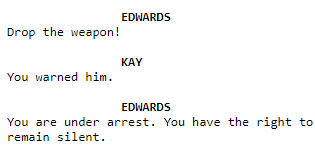
\includegraphics[width=1.0\textwidth]{data/pics/men in black.png}
\vspace*{-3mm}
\caption*{{\small \textbf{Excerpt from ``Men in Black'' (1997)}}}
\label{fig:2figsA}
\end{minipage}
\qquad
\begin{minipage}[t]{0.45\textwidth}
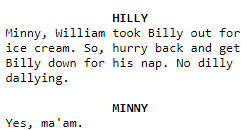
\includegraphics[width=0.9\textwidth]{data/pics/the help.png}
\vspace*{2mm}
\caption*{{\small \textbf{Excerpt from ``The Help'' (2011)}}}
\label{fig:2figsB}
\end{minipage}
\caption{Examples of conversations in the movie scripts.}
\label{fig:movie-script}
\end{figure}


\subsection{Related work}

In this section we give a brief overview of the existing conversational datasets of speaker's personal attributes and interpersonal relationships. We outline their shortcomings, which we addressed by collecting our own datasets.

\subsubsection{Datasets of demographic traits} 

Many conversational datasets labeled with personal attributes are not publicly available due to privacy protection of the speakers' data. The few accessible datasets include spoken dialogue transcriptions \cite{cieri2004fisher, love2017spoken} and artificially created conversations \cite{zhang2018personalizing, pers2}.

\citet{cieri2004fisher} gathered transcribed telephone dialogues on the given general topics; each speaker indicated their age, gender, dialect, education and occupation. \citet{love2017spoken} created a corpus of transcribed casual conversations of British English speakers, where all speakers specified their demographic (\textit{age}, \textit{nationality}, etc) and linguistic attributes (\textit{mother tongue}, \textit{dialect}). 

\citet{pers2} introduced an extension to the bAbI goal-oriented user-chatbot dialogue dataset \cite{bordes2016learning}, providing the users' ages, genders and food preferences. \citet{zhang2018personalizing} created a crowdsourced conversation dataset, Persona-Chat, where each speaker had to employ the given personality, described with a few sentences. A drawback of Persona-Chat is that it provides only textual descriptions of personas, as opposed to precise demographic facts. 
In general, the conversations created in a controlled way sound artificial, lacking of natural topic drifts and unnecessarily emphasizing the required content.  

\subsubsection{Datasets for relationship prediction} 

Two popular sources of conversational data for interpersonal relationship inference, are literary texts and movie scripts. Several studies provided the annotated relationships of the characters in novels as binary labels (positive or negative sentiment) \cite{chaturvedi2016modeling} or described as a bag-of-words \cite{iyyer2016feuding}. \citet{massey2015annotating} annotated the characters in literary texts with relationships on different granularity, additionally indicating the temporal change in relationship. 

Compared to literary texts, movie and series scripts provide dialogues in a structured format, simplifying speakers' identification. \citet{chen2020mpdd} collected conversations from Chinese TV series scripts and used three annotators to label them with 24 relationships and 7 emotions. The relationship labels were hierarchically split by field (\textit{family}, \textit{school}, \textit{company}, \textit{other}) and seniority (\textit{elder}, \textit{peer}, \textit{junior}). TV series scripts were also used by \citet{yu-etal-2020-dialogue}, where the script of Friends series was annotated by 2 judges with 36 predicates for relation extraction task, where 14 of the predicates indicated the relationship between people. \citet{jia2020ddrel} annotated relationships of the characters in the movie scripts with 13 relationship labels, belonging to four main categories (\textit{family}, \textit{intimacy}, \textit{official}, \textit{others}), resulting in the DDRel dataset. 

Unlike most prior works, we consider \emph{directed} relationships (e.g., \emph{parent} and \emph{child} as separate labels) and allow each speaker pair to have \emph{multiple} relationship labels. Moreover, our crowdsourced annotation is based on the fine-tuned agreement among at least 6 annotators, which provides more reliable aggregated results than in most related works.

\subsection{MovieChAtt dataset}
\label{data_moviechatt}

To overcome the limitations of the existing datasets of transcribed conversations we introduce \textit{Movie Character Attributes} dataset (MovieChAtt).
MovieChAtt is based on a subset of characters in the \gls{Cornell Movie-Dialogs Corpus} \cite{danescu2011chameleons} consisting of 617 movie scripts. From each movie, we derive a sequence of utterances for each character, excluding the characters who have less than 20 lines in the movie. We label the acquired characters with \textit{age}, \textit{gender}, and \textit{profession} attributes. The details on the attribute value lists and label distributions are given in Table \ref{moviechatt}; the overall dataset statistics are given in Table \ref{data_stats}. In the following we describe the labeling process for each personal attribute.

%\subsubsection{Preprocessing data} 

%Each utterance is represented as a sequence of words, excluding stop words, the 1,000 most common first names\footnote{Removed to prevent overfitting. The list of names is taken from \href{https://catalog.data.gov/dataset/baby-names-from-social-security-card-applications-national-level-data}{http://catalog.data.gov/dataset/baby-names-from-social-security-card-applications-national-level-data}}, and words that occur in fewer than four different movies.
%The latter two types of words are excluded in order to prevent the model from relying on movie-specific or character-specific signals that will not generalize. The rationale behind excluding rarely seen words is that the model could be prone to associate these words with characters' attributes, for instance, that `dinosaur' is an important attribute of a \textit{businessman} because of the dialogues in \textit{Jurassic Park}.


\begin{table*}[ht!]\sffamily
\centering
\begin{adjustbox}{width=0.95\textwidth}
\begin{tabular}{cccccc}
\textbf{Age}       & \textbf{Gender}          & \multicolumn{4}{c}{\textbf{Profession}}  \\ \toprule
adult (2645)       & female (959) & criminal (194)           & writer (45)     & manager (19)            & airplane pilot (12) \\
middle-aged (1183) & male (1003)  & military personnel (143) & unemployed (39) & banker (17)             & nurse (12)          \\
teenager (389)     &          & student (84)             & musician (36)   & school teacher (17)     & clerk (11)          \\
senior (220)       &          & child (83)               & lawyer (32)     & psychologist (17)       & professor (11)      \\
child (74)         &          & special agent (77)       & actor (32)      & journalist (16)         & photographer (9)    \\
                   &          & businessperson (71)      & politician (26) & waiter (16)             & activist (9)        \\
                   &          & policeman (66)           & priest (24)     & director (16)           & engineer (8)        \\
                   &          & housewife (66)           & astronaut (24)  & editor (15)             & painter (7)         \\
                   &          & doctor (63)              & assistant (24)  & salesperson (14)        & explorer (5)        \\
                   &          & scientist (58)           & sportsman (20)  & driver (14)             & stewardess (4)      \\
                   &          & detective (58)           & monarch (20)    & tv/radio presenter (13) &  
\end{tabular}
\end{adjustbox}
\caption{Lists of age, gender and profession attribute values in the MovieChAtt Dataset with value counts.}
\label{moviechatt}
\end{table*}

\subsubsection{Labeling age and gender} 

We extracted characters' \textit{gender} and \textit{age} attributes by associating the characters with their entries in the Internet Movie Database (\gls{IMDb}) and extracting the corresponding actor or actress' attributes at the time the movie was filmed, assuming that the gender of the actor and the character coincide in most cases.

This yielded 1,963 characters labeled with their genders and 4,548 characters labeled with their ages.
We discretized the age attribute into the following ranges:
(i) 0--13: \textit{child}, (ii) 14--23: \textit{teenager}, (iii) 24--45: \textit{adult}, (iv) 46--65: \textit{middle-aged} and (v) 66--100: \textit{senior}.
In our data the distribution of age categories is highly imbalanced, with \textit{adult} characters dominating the dataset (58.7\%) and \textit{child} being the smallest category (1.7\%).

\subsubsection{Labeling professions} 
\label{kappa1}

To obtain the ground-truth labels of characters' \textit{profession} attributes, we conducted a Mechanical Turk crowdsourcing task to annotate 517 of the movies in our corpus.
The workers were asked to indicate the professions of characters in a movie given
the movie's Wikipedia article.
The workers were instructed to select professions from a general predefined list if possible (e.g., \textit{doctor}, \textit{engineer}, \textit{military personnel}), and to enter a new profession label when necessary.
We manually defined and refined the list of professions based on several iterations of MTurk studies to ensure 
high coverage
and to reduce ambiguity in the options (e.g., \textit{journalist} vs \textit{reporter}).
We also included non-occupational ``professions'' that often occur in movies,
such as \textit{child} and \textit{criminal}.

Fleiss' kappa for the crowdworkers' inter-annotator agreement is $0.47$.
Disagreement was oftentimes caused by one character having multiple professions (Batman is both a \textit{superhero} and a \textit{businessman}), or a change of professions in the storyline (from \textit{banker} to \textit{unemployed}).
We kept only characters for which at least 2 out of 3 workers agreed on their profession,
which yielded 1405 characters labeled with 43 distinct professions.
The highly imbalanced distribution of professions, shown in Table \ref{moviechatt}, reflects the bias in our movie dataset, which features more \textit{criminals} and \textit{detectives} than \textit{waiters} or \textit{engineers}.

\subsection{FiRe dataset}
\label{relatinoship_dataset}

Addressing the need for a relationship dataset with \emph{directed, multi-label} interpersonal relationships of the conversation interlocutors we issue \textit{Film Relationship} dataset (FiRe). Compared to previous work, FiRe provides fine-grained relationship annotations, allowing multiple directed relationship labels per speaker pair. % We make FiRe publicly available at~\url{http://pkb.mpi-inf.mpg.de}.

\subsubsection{Data preparation}
We use the 
\emph{Jinni Movie Dataset}
collected in \citet{gorinski2018s}, which 
provides speaker labels for each utterance as well as the film genre metadata.
We selected the movies which:
\begin{itemize}[topsep=3pt,itemsep=2pt,partopsep=3pt, parsep=3pt]
    \item can be automatically associated with their Wikipedia page for annotation purposes
    \item have real-life genres, such as \emph{drama} or \emph{family}, to better approximate real-life conversations.
\end{itemize}
The selection of realistic movie scripts distinguishes FiRe from other character relationship datasets, such as in \citet{jia2020ddrel}. The model trained on FiRe 
is potentially more adaptive
to real-life dialogues.

For each pair of characters we kept only the film scenes where they are the only participants. Additionally, we include all uninterrupted dialogue spans of the considered pair in the 3-character scenes. We kept only the pairs which have at least 30 utterances throughout the whole movie.

\begin{table*}[h!]\sffamily
\centering
\begin{adjustbox}{width=0.95\textwidth}
\begin{tabular}{cccc}
\textbf{Family}       & \textbf{Social}          & \multicolumn{2}{c}{\textbf{Professional}}  \\ \toprule
parent (41)*                & friend (208)*                   & colleague/co-worker (67)*  &  boss/employer/master (29)* \\
child (48)*                 & enemy (27)*                    & doctor/patient (medical, 19)*       &  employee/servant (34)* \\
sibling (37)*               & (ex-)love interest (lover, 187)*       & client/seller (commercial, 19)*        &  religious relationship \\
(ex-)spouse (69)*           & fan                      & classmate       \\
engaged               & idol                     & teacher                \\
distant family member & members of the same club & student                \\
\end{tabular}
\end{adjustbox}
\caption[List of relationship labels split into categories.]{List of relationship labels split into categories. Labels marked with * are included in the final dataset and are supplied with number of acquired pairs.}
\label{relation-list}
\end{table*}

\subsubsection{Crowdsourcing annotation}

Inspired by \citet{massey2015annotating}, we manually created a list of 21 fine-grained relationships, divided into 3 categories: \emph{Family}, \emph{Social} and \emph{Professional} (Table \ref{relation-list}). %Some of the relationships are directed (for example, "parent"), for undirected ones (like "lover") we included "one-way relationship" tag, which indicates that only one of the characters experiences this relationship. 
We annotated character pairs in our dataset using MTurk, following the task design described in \citet{massey2015annotating}. For each character pair a worker was supposed to indicate all applicable relationships, given the links to the movie descriptions (Wikipedia and \gls{GradeSaver}, if available). Based on several pilot runs we opted to assign the labels agreed by 4 out of 6 annotators.

\subsubsection{Label aggregation}
\label{label_aggregation}
We selected the best label aggregation method based on the evaluation of several state-of-the-art models, ranging from the basic majority voting to the more complex resource-intensive methods.
To create the ground truth for comparison, 
we manually annotated 15\% of the pairs, retaining the labels on which 2 out of 3 annotators agreed.

We used an existing tool\gls{Crowdsourcing comparison tool by Zheng et al.} by \citet{zheng2017truth}\footnote{\href{https://zhydhkcws.github.io/crowd\_truth\_inference/index.html}{https://zhydhkcws.github.io/crowd\_truth\_inference/index.html}}, implementing state-of-the-art aggregation approaches, which enabled us to try out at least 7 different aggregation methods. We report the results of the best performing ones: 
\begin{itemize}
    \item David Skene model (DS) \cite{dawid1979maximum} is based on Expectation Maximizaion algorithm (EM), which jointly estimates the expertise of workers and the task label. This method has shown consistently optimal performance in many studies.
    \item Generative model of Labels, Abilities, and Difficulties (GLAD) \cite{whitehill2009whose} is an extension to EM that additionally estimates the difficulty of each task.
    \item Bayesian Classifier Combination (BCC) \cite{kim2012bayesian} uses Gibbs sampling to optimize the posterior joint probability of labels and workers.
\end{itemize}
We compare them to the majority voting (MV) approach. Note, that most of the models are based on the assumption of single-label answers, so we had to reformulate the problem as multiple binary-decision problems to fit them.

Taking into account that each pair can have multiple labels associated with it and that the agreement can be reached only on a subset of those labels, we propose to evaluate both \emph{partial} accuracy (the workers' answers partially match the golden set) and \emph{total} accuracy (the workers' answers and the golden set are identical). Additionally, we evaluate precision and recall for all approaches. The results are shown in Table~\ref{tab:aggregation}. 

\begin{table}[]
    \centering
    \begin{adjustbox}{width=0.6\textwidth}
    \begin{tabular}{@{}lrrrr@{}}
            & \textbf{partial accuracy} & \textbf{total accuracy} & \textbf{precision} & \textbf{recall} \\ \toprule
\textbf{MV} & \textbf{0.98}                    & \textbf{0.68}                  & \textbf{0.88}                 & 0.76             \\
GLAD        & \textbf{0.98}                             & 0.67                           & \textbf{0.88}                          & 0.76                       \\
DS          & 0.97                             & 0.59                           & 0.79                          & 0.82                       \\
BCC         & \textbf{0.98}                             & 0.67                           & 0.83                          & \textbf{0.85}                      
\end{tabular}
    \end{adjustbox}
    \caption{Comparison of answer aggregation methods.}
\label{tab:aggregation}
\end{table}

The compared models show almost equal performance, with MV having the greatest total accuracy and BCC yielding the best recall. We opted to use MV aggregation, as we consider high precision and accuracy more important for this task; additionally, MV is easier to interpret. One reason why the iterative approaches do not outperform simple majority voting is that most MTurk workers label only 1-2 pairs, which is too few for the iterative models to effectively infer the workers' expertise.

To further ensure the high quality of our annotated data,
we used the Honeypot method~\cite{lee2010social}, where the questions with the known true answers (honeypots) are mixed into the task. The workers' scores are calculated as the fraction of their correct answers to the honeypots; the workers who did not get any honeypots were assigned an average score. After that all worker's answers are scaled by the obtained scores and the label was considered as correct if the sum of its votes exceeded a threshold, finetuned on the annotated set.

\subsubsection{Dataset analysis}

We obtained a multi-label Fleiss kappa of 0.45, which corresponds to moderate agreement. In total we collected 783 annotated character pairs from 254 films, of which 5\% are labeled with $\ge 2$ relationships. The original set of labels was filtered to include only those which have at least 20 representative samples, resulting in 12 labels. Summary statistics of the final dataset are given in Table \ref{data_stats} and the relationship label distribution in Table \ref{relation-list}. We observed that the label distribution is heavily biased towards \emph{friend} and \emph{lover} labels, encountered almost 3 times more often than the third most popular label \emph{spouse}.

\subsubsection{Series dataset}

We created an additional dataset of labeled TV series scripts, which are different from film screenplays, because they contain a longer history of interactions. The scripts of the series were crawled from \gls{IMSDb}. As there is no information about scene boundaries in the gathered scripts, for each given character pair we kept only the uninterrupted sequences of at least 7 utterance turns. 

For the resulting dataset we selected the series which would be realistic and diverse in topics. Following the same crowdsourcing annotation procedure as for FiRe, we collected 365 labeled pairs with 0.33 Fleiss' kappa agreement; the dataset statistics are included in Table~\ref{data_stats}. Compared to FiRe, character pairs in this dataset have larger number of utterances, around four times as much on average.

\begin{table}[]
    \centering
    \begin{adjustbox}{width=0.65\textwidth}
    \begin{tabular}{@{}lrrrrrr@{}}
                  & \multicolumn{2}{c}{\textbf{MovieChAtt}}  & \multicolumn{2}{c}{\textbf{FiRe}} & \multicolumn{2}{c}{\textbf{Series}}                           \\
                    \cmidrule(lr){2-3} \cmidrule(l){4-5} \cmidrule(l){6-7}
                    & \textbf{avg}      & \textbf{max}        & \textbf{avg}      & \textbf{max} & \textbf{avg}      & \textbf{max} \\ \toprule
words per utterance & 11 & 556 & 13           & 602        & 13                          & 340                     \\
utterances per pair & 79 & 471 & 99           & 597        & \multicolumn{1}{r}{417}     & 15,216                   \\
words per pair  & 823 & 7798    & 1,087        & 3,977      &        6,562              &  188,676     
\end{tabular}
\end{adjustbox}
    \caption{Statistics for MovieChAtt, FiRe and Series datasets.}
    \label{data_stats}
\end{table}

\subsection{Discussion}

Although the dialogues in films resemble real-life conversations, they sometimes sound artificial and allegorical, being produced from an existing script and well-rehearsed. Compared to real conversations, the interactions in the movies usually contain less colloquial speech, abbreviations and dialect words, so that they are more understandable to the general audience. Another drawback of using movie data is that many films have unrealistic elements in their plot, which can not be completely handled by our proposed genre filtering. Finally, the distribution of labels for some personal attributes in the movies do not follow those in real life (for example, big bias towards \textit{lover/friend} relationships or heroic professions).






\section{Social media submissions}

%\subsection{Introduction}

Reddit is a popular social media platform for discussing a wide range of topics. It has become an prominent source of information for data analysis on social media as it provides an abundance of data with rich structure and covers a broad range of topics. Such data has many applications, including personalizing healthcare \cite{gyrard2018personalized}, recommendations, search, and conversational agents. 
Reddit is used by approximately 330 million users\footnote{{\scriptsize \url{https://redditblog.com/2018/11/13/holiday-on-reddit/}}}
with 2.8 million comments written each day\footnote{{\scriptsize \url{https://www.digitaltrends.com/social-media/reddit-ads-promoted-posts/}}}. 

Despite its popular and abundant data, few have considered Reddit as a source of data for inferring users' personal traits. However, many Reddit submissions contain a sufficient amount of personal information; an exemplary submission, indicating the user's hobby, is shown in Figure \ref{fig:input}. Prior work has focused on Reddit as a source of demographic information, whereas rich attributes, like profession and hobbies, are usually overlooked. 

\begin{figure}[th!]
\centering

\includegraphics[width=0.58\textwidth]{pics/brew.png}
\caption{
Example of a Reddit post.
%Cues in bold suggest \emph{brewing} as the user's hobby.
}
\label{fig:input}
\end{figure}

We address this gap by creating a labeled dataset of Reddit users \footnote{Available at {\scriptsize \url{https://www.mpi-inf.mpg.de/departments/databases-and-information-systems/research/pkb}}.}
(including their posts and comments) that covers five user attributes: \textit{profession, hobby, family status, age,} and \emph{gender}. The collected submissions can be used as a proxy for dialogue utterances in conversational data research.
%We leveraged three high-precision approaches to identify predicates and their object values in users' posts: \textit{(1)} natural language patterns matching assertions like \textit{I am a flight attendant}, \textit{(2)} bracket patterns matching structured assertions of users' ages and genders (\textit{I [35m] just broke up with my girlfriend}), and \textit{(3)} flair metadata specific to particular subfora. We used human judgments to validate the high-precision nature of these approaches before performing an analysis of the resulting dataset. 

\subsection{Related work}

Automatic methods for identifying users' personal attributes 
from social media focus on user-generated content from Twitter, with a few exceptions that explore Facebook \cite{sap:EMNLP14,Schwartz2013PersonalityGA} or Reddit \cite{fabian2015privacy,finlay2014age,gjurkovic-EtAl:2018} posts.
Such methods, particularly supervised learning approaches, require a collection of user-generated content labelled with personal attributes of interest.

Data collection for such models is mostly done via: manual annotation after a focused search with specific keywords or hashtags \cite{pietro:ACL15,Rao:2010}, public profile linked to Twitter profile description \cite{burger:EMNLP11,flekova:ACL16:long}, self-reports as part of an online survey \cite{finlay2014age,flekova:ACL16:long,pietro:ACL17:long,pietro:COLING18,sap:EMNLP14,schwartz2013personality}, or pattern-based extraction approach 
(e.g., \texttt{\small(I$|$i) (am$|$'m$|$was) born in + number (1920-2013)}) on user profile description or user posts \cite{fabian2015privacy,kim:ACL17:short,sloan2015tweets,tigunova2019listening}.
Several works \cite{basile:2017,bayot:MOD17} made use of labelled datasets published within the shared task on \textit{author profiling} organized by the CLEF PAN lab \cite{stein:2017o,stein:2017l}. 

There has been less effort on identifying demographic attributes of Reddit users compared with the body of work that exists for Twitter users. However Reddit posts have been exploited for other purposes, such as determining \emph{users' personality} \cite{gjurkovic-EtAl:2018}, \emph{mental health condition} \cite{cohan2018smhd}, \emph{domestic abuse} \cite{schrading2015analysis} and \emph{irony detection} \cite{wallace2014humans}, among others.
\citet{thelwall2018she} investigate how the topic of subreddit influences the gender ratio within it. The study was performed on 100 subreddits grouped by interest, gender information about the users were collected by guessing it from their usernames, which is arguably a low-precision strategy. Smaller scale Reddit datasets exist for \emph{gender}, \emph{age} and \emph{location} attributes \cite{fabian2015privacy,finlay2014age}, which are unfortunately not publicly available. As far as we know, we are the first to consider \textit{hobby} as a personal attribute of interest to be identified from online communication.

\subsection{Background}

%Reddit\footnote{{\scriptsize \url{https://www.reddit.com/}}} is a social news website and forum where registered members can submit content including links, text posts, and images, which are then voted up or down by other members.
%Before elaborating on the creation of our dataset derived from Reddit posts, we describe several concepts on Reddit that are relevant for the data collection process.

\paragraphHd{Posts and Comments.}
Discussions on Reddit are organized in threads, which are initiated by an original \textit{post} and may contain \textit{comments} replying to the post and to the other comments. This creates a hierarchical structure that resembles a conversation between the users.
Both posts and comments can be a textual content, a link with anchor text or images.

\paragraphHd{Subreddits.}
Reddit is organized into subreddits, which are fora that focus on specific topics.
Those can be split by interest (sports, politics, etc), by country or community, type of content (text, gifs, videos), and so on. Subreddits have their own rules, but any registered user can create them. By convention, subreddits are prefixed with \texttt{\small /r}. For example, users discuss hockey in the \texttt{\small /r/hockey} subreddit.

\paragraphHd{Flairs.}
Flair is a user or post metadata that is a unique feature of Reddit. Flair is a small image with a short text description that is attached to a post or a username. Flairs can be defined differently for specific purposes by each subreddit. For example, in \texttt{\small /r/travel} subreddit they may indicate the \textit{country} of the user, \textit{gender} in \texttt{\small /r/AskMen} and \texttt{\small /r/AskWomen} or users' \textit{favorite teams} in \texttt{\small /r/hockey}.
Flairs for posts can be useful to filter and search for a particular content.

\subsection{RedDust dataset}

In this section we describe the creation of our proposed \emph{RedDust} dataset, containing a collection of Reddit users. Each user in the dataset is associated with posts and comments they produce (which we call \textit{submissions} in the following) and users' inferred personal attributes.
We considered five personal attributes including \textit{gender}, \textit{age}, \textit{family status}, \textit{profession} and \textit{hobby}.
The dataset is created from the openly published \gls{Reddit dump}\footnote{ \href{https://files.pushshift.io/reddit}{https://files.pushshift.io/reddit}}, which spans between 2006 and 2018. 

There are several criteria on which users and submissions are included in RedDust, i.e., users who posted between 10 and 100 submissions, and submissions containing between 20 and 100 terms after filtering. We filtered out hyperlinks and user mentions (i.e., \texttt{\small @nickname}) from the original content.

Some subreddits are likely to contain many false positives, such as those concerned with video games or role playing. This leads to personal assertions talking about the users' projected persona in a particular context (e.g., \textit{``I am a priest looking for a guild''}). To mitigate this source of false positives, we blacklisted subreddits about gaming, fantasy and virtual reality from the top 500 subreddits sorted by the number of unique users. Posts made to blacklisted subreddits were discarded. 
Similarly, we discarded posts that contain quotations in order to reduce the possibility of the user referring to a third person (\textit{``... and he shouted `Hands on the counter, I am a cop!' ''}).

For attributes that usually have a unique value (i.e., \textit{gender}, \textit{age} and \textit{family status}) we also exclude users who state multiple different values to avoid introducing false positives. Meanwhile, we allow each user to have multiple attribute values for \textit{profession} and \textit{hobby}. The age of a given user is calculated relative to his or her age when writing the most recent comment. In the following we discuss particular techniques used to extract values for each personal attribute.

\subsubsection{Gender}
Gender has been the most popular user attribute to predict in existing user profiling work, particularly on Reddit \cite{fabian2015privacy,thelwall2018she,Vasilev2018}.
In 
RedDust
we consider gender as a binary predicate (\emph{female} or \emph{male}) 
as has been done in prior work. 

Instead of considering usernames as a means for gender classification, as was done by \citet{thelwall2018she}, we look for self-reported gender assertions, which provide labels of higher precision.
Specifically, we identified 
users' gender
using the following methods:
\begin{itemize}
    \item \textbf{Natural language patterns}.
    Following \citet{fabian2015privacy}, we manually created a set of patterns that indicate a specific gender. They have the general form of \texttt{\small (I am|I'm) a? <gender indicator>}, meaning that matches should contain `\textit{I am}' or `\textit{I'm}', optionally followed by an article `\textit{a}', then a word that indicates gender like `\textit{man}' or `\textit{mother}'. A comprehensive list of patterns we used is given in Table \ref{pat_table}, and the indicative gender words are shown in Table \ref{word_table}. Although the gender of a given user can be expressed in a longer snippet like ``\textit{I am a great mother}'', we do not allow extra words like \textit{great} to appear before gender-indicating words. This reduces false positives from statements like ``\textit{I'm a far cry from my mother}''.
    
    \item \textbf{Bracket patterns}.
    In certain situations, users often volunteer to indicate their demographic information in order to give their posts more context (``\textit{I [30f] was dating this guy [35m]...}'').
    This is common in relationship-related subreddits, where the users' age and gender are often relevant to the discussions. These cues are generally written in round or square brackets. To reduce false positives, we do not consider such patterns when they appear without brackets. To capture gender and age expressed in this way, we look for patterns of the form \texttt{\small (I|I'm|me) [<number>(m|f)]}.
    
    \item \textbf{Flairs}.
    Like \citet{Vasilev2018}, we also consider gender-indicating flairs attached to users.
    This logic is subreddit-specific, so we restrict ourselves to common subreddits.
    For example, in subreddits \texttt{\small /r/AskWomen} and \texttt{\small /r/AskMen} the flair is one of \textit{male, female, trans}, and so on, whereas in \texttt{\small /r/tall} and \texttt{\small /r/short} the flair is either \textit{pink, blue}, or \textit{other}.

\end{itemize}

\subsubsection{Age}
We label users' posts with age predicate using similar techniques as for gender:

\begin{itemize}
    \item \textbf{Natural language patterns}.
    To infer users' age, we utilized five patterns listed in Table \ref{pat_table}, with pattern (v) specifically designed to avoid false positives as in ``\textit{I am 6 feet tall}''.
    We then calculated the exact age for patterns (i)-(iii) by subtracting the birth year from the publishing year of the post containing such patterns.

    \item \textbf{Bracket patterns}.
    Numbers indicating age were jointly collected along with gender, as described in the above-mentioned bracket patterns for gender.
\end{itemize}

Finally, we made sure that the obtained ages for users in RedDust are within the range of 10-100 years old, since users under 13 are not allowed to register and there are unlikely to be many users above 100 years old.
This is helpful for reducing false positives, such as those in conditional sentences (``\textit{as if I were 5 years old}'').

\subsubsection{Family status}

We consider family status as a binary predicate indicating whether a person is \emph{single} or has a \emph{partner}. Similar to labeling gender, we relied on natural language patterns containing indicative words, which are detailed in Table \ref{pat_table} and \ref{word_table}, respectively. We distinguished two cases of indicative words: (i) \textit{{self-status indicator}}, used when the speaker refers to her own status (\emph{``I am divorced''}); and (ii) \textit{{partner indicator}}, when the speaker refers to the existence of a partner (\emph{``My boyfriend''}).

We additionally collected matches of negated patterns of both (i) and (ii)
%,i.e.,\texttt{\small I am not <self-status indicator>} and \texttt{\small I don't have a  <partner indicator>}
in order to expand the labelled data. Furthermore, given that the indicator word \emph{single} is often used in a more general context (e.g., `\emph{single player}', `\emph{single bed}'), we restricted the patterns containing this particular word, so that it should be immediately followed by punctuation, conjunctions or few allowed words like `\emph{father}'.

\begin{table*}[t!]
\centering
\begin{adjustbox}{width=0.88\textwidth}
\begin{tabularx}{\linewidth}{ll}
\toprule
\textbf{attribute} & \textbf{pattern(s)} \\
\midrule
gender & \texttt{\footnotesize (I am|I'm) a? <gender indicator>} {\footnotesize(e.g., \emph{man}, \emph{mother})} \\ [0.8ex] 
age & (i)\quad \texttt{\footnotesize I (was|am) born in <four digit year>} \\ 
 & (ii)\quad \texttt{\footnotesize I (was|am) born in <two digit year>} \\
 & (iii)\quad \texttt{\footnotesize I was born on <day, month, year>} \\
 & (iv)\quad \texttt{\footnotesize I am <number> years old} \\
 & (v)\quad \texttt{\footnotesize I am <number>} {\footnotesize immediately followed  by punctuation or conjunction} \\ [0.8ex]
family status & (i)\quad \texttt{\footnotesize I am <self-status indicator>} {\footnotesize (e.g., \textit{divorced}, \textit{single})} \\
 & (ii)\quad \texttt{\footnotesize (my|I have a) <partner indicator>} ({\footnotesize e.g., \textit{wife}, \textit{boyfriend})} \\ [0.8ex]
profession & \texttt{\footnotesize (I am|I'm) a <profession name>} \\ [0.8ex]
hobby & \texttt{\footnotesize <phrase indicator>} {\footnotesize (e.g., \textit{I enjoy}, \textit{I like})} \texttt{\footnotesize <hobby name>} \\ [0.8ex]
\bottomrule
\end{tabularx}
\end{adjustbox}
\caption{Patterns for labeling Reddit users with personal attributes.}
\label{pat_table}
\end{table*}


\begin{table*}
\centering
%\small
\begin{adjustbox}{width=0.88\textwidth}
\begin{tabularx}{\linewidth}{llX}
\toprule
\textbf{attribute} & \textbf{value} & \texttt{\footnotesize word/phrase indicators} \\
\midrule
gender & female & \textit{woman}, \textit{female}, \textit{girl}, \textit{lady}, \textit{wife}, \textit{mother}, \textit{sister} \\
 & male & \textit{man}, \textit{male}, \textit{boy}, \textit{husband}, \textit{father}, \textit{brother}
 \\ [1.0ex]
family status & single & \texttt{\footnotesize self-status}: \textit{single}, \textit{divorced}, \textit{widow}, \textit{spouseless}, \textit{celibate}, \textit{unmarried},  \textit{unwed},  \textit{fancy-free} \\
 & partner & \texttt{\footnotesize self-status}: \textit{married}, \textit{engaged}, \textit{dating} \\
 & & \texttt{\footnotesize partner}: \textit{boyfriend}, \textit{spouse}, \textit{girlfriend}, \textit{fiancee}, \textit{lover}, \textit{partner}, \textit{wife}, \textit{husband}
  \\ [1.0ex]
hobby & - & \textit{my hobby is}, \textit{I am/I'm fond of}, \textit{I am/I'm keen on}, \textit{I like}, \textit{I enjoy}, \textit{I go in for}, \textit{I take joy in}, \textit{I adore,} \textit{I love}, \textit{I play, I fancy}, \textit{I am/I'm a fan of, I am/I'm fascinated by}, \textit{I am/I'm interested in}, \textit{I appreciate, I practise}, \textit{I am/I'm mad about} \\
\bottomrule
\end{tabularx}
\end{adjustbox}
\caption{Words and phrases considered as indicators used in patterns for labeling personal attributes.}
\label{word_table}
\end{table*}

\subsubsection{Profession}
To obtain profession labels we consulted a list of occupation names from Wikipedia\footnote{ \href{https://en.wikipedia.org/wiki/Category:Lists\_of\_occupations}{https://en.wikipedia.org/wiki/Category:Lists\_of\_occupations}} and recursively added all titles under subcategories. The resulting list consists of about 1K professions and contains a lot of fine grained occupations, some of which are redundant or ambiguous. Our strategy is to capture as many profession assertions as possible, giving users of RedDust the opportunity to filter and group the professions depending on their specific use cases.

Each profession in the list was considered as \texttt{\small profession name} in the pattern \texttt{\small (I am|I'm) a <profession name>} that we used to label Reddit users with the \emph{profession} attribute.
After performing pattern matching against the whole Reddit dataset, we were left with 832 unique profession names in RedDust.

\subsubsection{Hobby}
Similar to collecting names of professions, we obtained a list of hobbies from Wikipedia\footnote{ \href{https://en.wikipedia.org/wiki/List_of_hobbies}{https://en.wikipedia.org/wiki/List\_of\_hobbies}} and 
utilized them as \texttt{\small hobby name} in our natural language patterns for the \emph{hobby} attribute.
We used a diverse set of patterns of the form \texttt{\small <phrase indicator> <hobby name>}, where \texttt{\small phrase indicator} is a phrase like `\textit{my hobby is}' or `\textit{I enjoy}', as listed in Table \ref{word_table}. 
Using the pattern matching approach, users in RedDust were labeled with 336 unique hobby names in total.

\begin{table}[h!]\sffamily
\centering
\small
\begin{adjustbox}{width=0.6\textwidth}
\begin{tabular}{lccc}
\toprule
\textbf{attribute} & \textbf{precision} & \textbf{\#false positives} & \textbf{\#disagreements} \\
\midrule
gender & 0.96 & 2 & 2 \\
age & 1.0 & 0 & 2 \\
family status & 0.86 & 7 & 8 \\
profession & 0.96 & 2 & 2 \\
hobby & 0.94 & 3 & 9 \\
\midrule
avg/total & 0.94 & 14 & 23 \\
\bottomrule
\end{tabular}
\end{adjustbox}
\caption{Number of false positives and inter-rater agreement on RedDust.}
\label{agreement}
\end{table}

\subsubsection{Labeling evaluation}
\label{kappa2}
To validate the high-precision nature of our labeling approach, we asked three human annotators 
to verify the correctness of labels for each predicate. We randomly sampled 50 labeled posts for each attribute and asked annotators to indicate whether the given label matched the user's actual assertion. The decision to accept or reject the label was based on a majority vote from the annotators.

The results of this human evaluation are shown in Table \ref{agreement}. In total there were 23 instances without perfect annotator agreement (out of 250 total instances for five attributes), which indicated 14 false positives after taking a majority vote. Half of these false positives came from the family status attribute, due to ambiguous usage of words like 
`\emph{partner}' in statements like ``\emph{I have a partner in this crime}''.
Despite such false positives, 
the average labeling precision for all personal attributes in RedDust is 94\%.
Furthermore, we also measured annotator agreement with Fleiss' kappa as 0.67 on average for all attributes, which indicates a substantial agreement; the worst agreement (0.59) was reached for the \textit{family status} attribute.

\subsection{Data statistics and analysis}

In this section we present the quantitative and qualitative analysis of the RedDust resource. In Table \ref{stats_table} we present the overall
statistics of the dataset. Figure \ref{num_posts} shows the chart of the user count per each post count. From this plot we conclude that the users in our dataset tend to have a small number of posts.

\begin{table}[h!]%\sffamily
\centering
\small
\begin{adjustbox}{width=0.55\textwidth}
\begin{tabular}{lrrr}
\toprule
\textbf{attribute} & \textbf{\#users} & \textbf{\#posts} & \textbf{\#subreddits} \\
\midrule
gender & 54.88K & 2.49M & 28.25K \\
age & 122.20K & 5.80M & 44.07K \\
family status & 11.77K & 0.56M & 14.76K \\
profession & 74.86K & 3.63M & 37.49K \\
hobby & 89.07K & 4.42M & 41.31K \\
\midrule
total & 352.78K & 16.9M & 165.88K \\
\bottomrule
\end{tabular}
\end{adjustbox}
\caption{Overall RedDust statistics for each attribute.}
\label{stats_table}
\end{table}

\begin{figure}[!h]
\centering
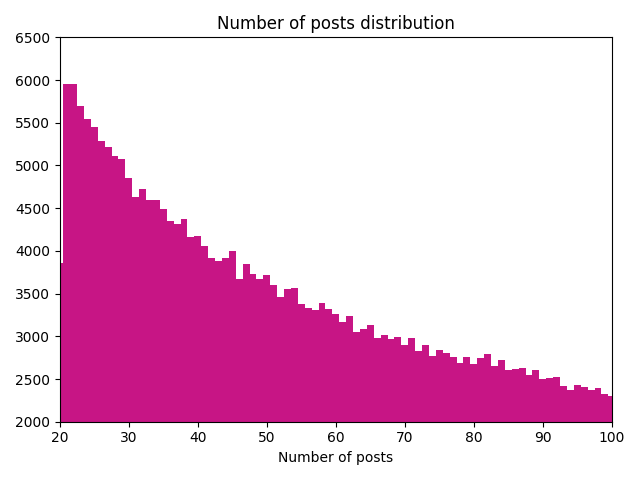
\includegraphics[width=0.55\textwidth]{data/pics/num_posts.png}
%\vspace*{-0.3cm}
\caption{Counts of users having $x$ number of Reddit posts.}
\label{num_posts}
\end{figure}

Almost 19K users in RedDust have two personal attributes known, 980 users have three and 28 have four attributes known,
which amounts to 6\% of the users having multiple personal attributes in total.
For  
such users
it is interesting to look at the interplay between different personal traits, for instance, the correlation between users' occupations and general interests.
In Figure \ref{prof-hob} we plot a heat map which represents the co-occurring values for these two predicates. 
For this experiment as well as the subsequent ones, we limit the number of professions and hobbies to the top $k$ ones ($k=20$ and $k=30$ for \textit{profession} and \textit{hobby}, respectively), sorted by the number of labeled users per value.

We observed intuitive correlations such as:
\emph{musicians} often play \emph{guitar};
\emph{runners} have \emph{running} as the main interest; 
\emph{college students} like to \emph{read} but are also interested in \emph{video games} five times as much as any other professions;
and curiously, \emph{shooting} is popular among \emph{photographers}, most probably because of \textit{shooting} being an ambiguous term.

\begin{figure*}[]
  \centering
  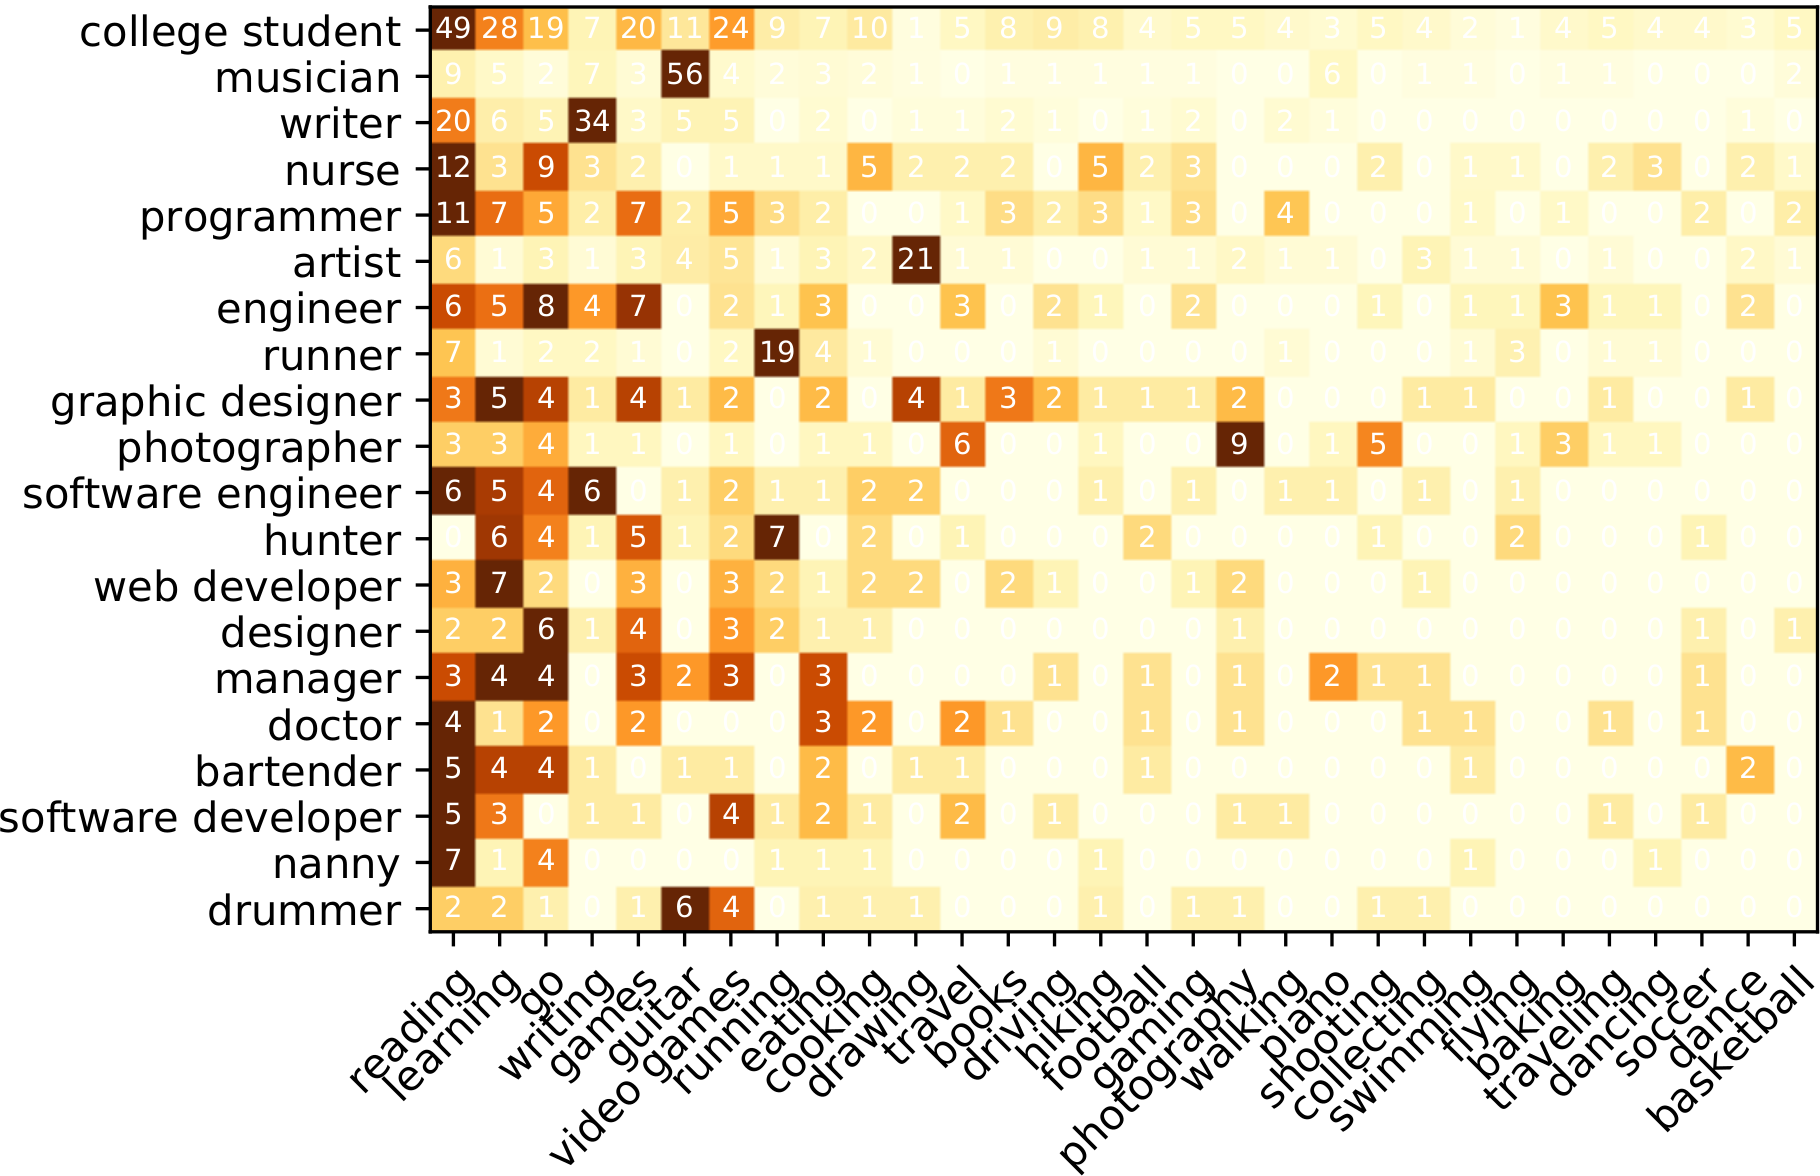
\includegraphics[width=0.77\linewidth]{data/pics/hob_prof.png}
  \caption{Co-occurrence of the most common professions and hobbies.}
  \label{prof-hob}
\end{figure*}

We also considered other pairs of attributes, namely \textit{profession} and \textit{gender}, for which we show the gender distribution of each profession in Figure \ref{prof_gender}. 
The analysis revealed common prejudices like \emph{female nannies} or \emph{male programmers},  
as well as several surprising insights (prevalence of \textit{female runners} and \textit{bartenders}) possibly specific to Reddit communities.

\begin{figure*}[]
\centering
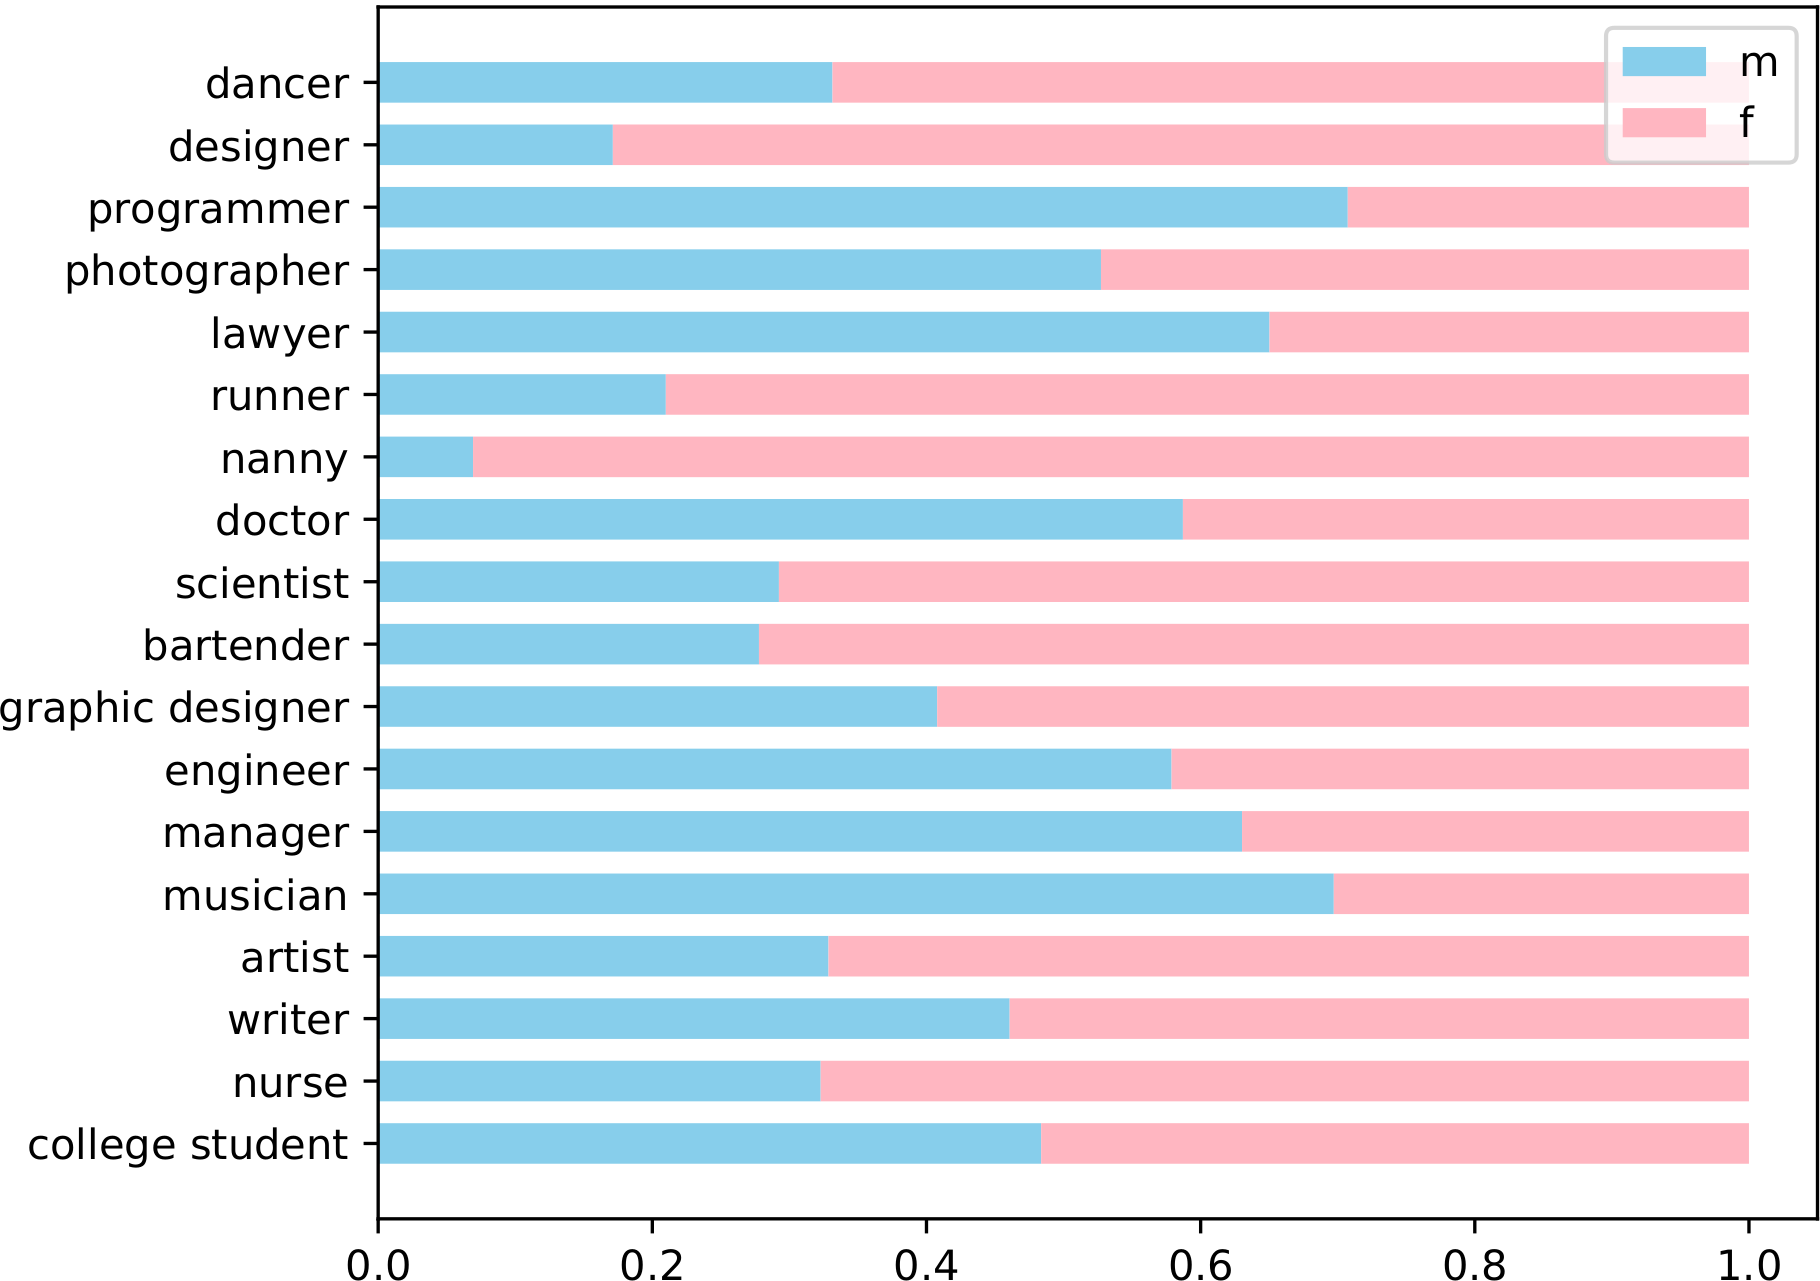
\includegraphics[width=0.67\linewidth]{data/pics/prof_gend.png}
\caption{Gender distribution among professions.}
\label{prof_gender}
\end{figure*}


\subsection{Labeling Reddit data with weak supervision}

While using explicit statements in brackets (e.g. [35f] indicating a \textit{35-year-old female}) and flairs is a reliable way to get age and gender of the users, utilizing natural language patterns (e.g. \textit{I am a doctor}) is a much nosier method, producing many false positive errors. In addition to that, the explicit assertions, required for the pattern-based approach are rare, because the users usually hint to their personal traits with subtler cues (for example, a profession \textit{doctor} can be deduced from the frequent use of medical terms in the posts). 

Keeping in mind these limitations of the natural language pattern-based approach we turn to the \textit{weak supervision} method to create a refined dataset for \textit{hobby} and \textit{profession} user traits. 

\paragraphHd{Snorkel.} We used the Snorkel framework \cite{ratner2017snorkel}, which allows data labeling using weak supervision. 
Snorkel does not require manual evaluation of each data sample, instead it relies on the outputs of multiple \textit{labeling functions}, such as patterns or heuristics, which are manually specified and can be potentially noisy. The accuracies and correlations of the labeling functions are then estimated by automatically deriving the \textit{generative model} over the labeling functions. The generative model weights and combines the outputs of labeling functions to produce final list of probabilistic labels.

\vspace{10pt}

We modified the criteria for including Reddit submissions, so that they are:
\emph{(1)} authored by users having 10-50 posts, \emph{(2)} 10-40 words long, and \emph{(3)} containing a personal pronoun (except for 3rd person ones).
Requirements \emph{(1)} and \emph{(2)} were derived from observing the word and post distributions on the full dataset.
Requirement \emph{(3)} comes from the assumption that posts containing personal pronouns are most likely to contain personal assertions. These restrictions allow us to select posts that look more similar to the real conversation (i.e., relatively short and containing references to the speakers with personal pronouns).
In addition, we did not consider the following subreddit types: \emph{(i)} \emph{dating}, which may provide plenty of personal information but no real conversation to infer from,
and \emph{(ii)} \emph{fantasy/video games} (for the \emph{profession} attribute), because users may refer to gaming personalities.
We selected only the users whose utterances contain at least one mention of the attribute values, from the Wikipedia lists of professions and hobbies,
resulting in around 250K and 500K candidate users for profession and hobby, respectively.

We then input the collected users into the Snorkel framework. Given a user's utterance set $U$, an attribute $a$ and a possible attribute value $v$, Snorkel will decide on a \emph{positive}/\emph{negative} label--denoting the user as having/not having personal trait~$a$~:~$v$; or if the decision can't be made -- an \emph{abstain} label.%, by combining multiple noisy outputs from the labeling functions with a probabilitsic model.

We have separate labeling models for each attribute $a$, and defined two labeling functions which consider: \emph{(LF1)} the existence of the \emph{attribute-specific patterns}, and \emph{(LF2)} the weighted count of the words belonging to the \emph{value-specific lexicon}.

\paragraphHd{LF1: Attribute-specific patterns.} We compiled a list of positive and negative patterns for each attribute (see Table \ref{tab:patterns}), e.g., \emph{``my hobby is $\langle$hobby-value$\rangle$''} vs \emph{``I hate $\langle$hobby-value$\rangle$''} as positive vs negative patterns for hobby.
LF1 labels a user with a \emph{positive/negative} label for each attribute value $v$ if there exist at least one positive/negative pattern in the user's utterances $U$, and \emph{abstain} otherwise.

\begin{table}[t!]
\centering
\small
\begin{adjustbox}{width=0.95\textwidth}
\begin{tabular}{@{}lllll@{}}
\toprule
\multicolumn{2}{c}{\textit{\textbf{profession}}} & \multicolumn{3}{c}{\textit{\textbf{hobby}}}                     \\ \midrule
\textbf{positive}       & \textbf{negative}      & \multicolumn{2}{c}{\textbf{positive}} & \textbf{negative}       \\ \midrule
 \begin{tabular}[t]{@{}l@{}} i am/i'm a(n)\\my profession is\\i work as\\my job is\\my occupation is\\i regret becoming a(n)  \end{tabular}                                                   & \begin{tabular}[t]{@{}l@{}} (no/not/don't \\within pos. patterns)  \end{tabular} 
 & \begin{tabular}[t]{@{}l@{}} i am/i'm obsessed with\\i am/i'm fond of\\i am/i'm keen on\\i like\\i enjoy\\i love\\i play\\i take joy in\\i adore\\i appreciate\\i am/i'm fan of \end{tabular}  
  & \begin{tabular}[t]{@{}l@{}} i am/i'm fascinated by\\i am/i'm interested in\\i fancy\\i am/i'm mad about\\i practise\\i am/i'm into\\i am/i'm sucker for \\ my interest is\\ my hobby is\\ my passion is\\ my obsession is \end{tabular}  
 &  \begin{tabular}[t]{@{}l@{}} i hate\\i dislike\\i detest\\i can't stand \\ (never/not/don't \\within pos. patterns) \end{tabular}  \\
\bottomrule
\end{tabular}
\end{adjustbox}
\caption{Positive and negative patterns used in the labeling function LF1 of the Snorkel labeling model. Each pattern must be followed by possible attribute values within a context window of 2 terms.}
\label{tab:patterns}
\end{table}


\paragraphHd{LF2: Value-specific lexicon.} For each attribute-value pair, we used \textit{Empath} \cite{fast2016empath} --pre-trained on the Reddit corpus-- to build a lexicon of \emph{typical words} (e.g., `cider' and `yeast' for \emph{hobby:brewing}). Given seed words, Empath builds lexical categories by means of an embedding model. As our value-specific lexicon, we took the union of Empath terms for a specific attribute value and all its synonyms; each typical word is weighted by embedding similarity to the seed words. 
Given a user's utterance set $U$ and an attribute value $v$, LF2 yields a \emph{positive} label if the weighted count of typical words of $v$ is above an empirically-chosen threshold, and \emph{abstain} otherwise.

\vspace{5pt}
Given a pair of user's utterance set $U$ and a possible attribute value $v$, the Snorkel probabilistic labeling model utilizes our labeling functions to
predict a confidence score for the \emph{positive} label, i.e., the user is labeled with attribute value $v$.
As our labeled dataset, we took only the user-value pairs with confidence scores above a specific threshold. 

To determine the threshold of confidence scores, we manually annotated a held-out validation set containing 100 users per attribute. 
Given a post and a set of attribute values mentioned explicitly in the post, the annotators had to identify whether the candidate user traits truly hold. For instance, from \emph{``My dad bought me a \textbf{chess} board even though I enjoy \textbf{video games} more''}, \emph{hobby:video games} is correct while \emph{hobby:chess} is not applicable.
The final annotation for each post consists of attribute values agreed by at least two out of three judges. The selected confidence threshold corresponds to the 0.9 precision of the model on the validation set. After thresholding, we obtained 13.5k users labeled with profession values and 11.7k users with hobby values.

To demonstrate that Snorkel provides the same level of quality as crowdsourcing,
we calculated the precision of human annotators
on the same validation set by comparing
the labels of each annotator against the agreement
labels. The obtained precision scores were 0.91 for
profession and 0.88 for hobby, demonstrating that
Snorkel is a reasonable alternative to crowdsourcing.



\subsection{Discussion}

Automatically labeling social media posts is an efficient and low-cost way to collect labeled conversations at scale. However, this approach only works for specific attributes (e.g. it is infeasible to collect \textit{relationships} among Reddit users, because most of them are strangers to each other). Another drawback of using social media platforms is the biased user demographics distribution, such as prevalence of young people or several professions being underrepresented. Moreover, the labels obtained from pattern search are much noisier than the crowdsourced ones, requiring further manual revision steps. Finally, the automatically collected Wikipedia attribute value lists can be further refined, merging redundant values and adding the missing ones.

\chapter{Hidden Attribute Models}
\label{chap_ham}
\minitoc
%personal information in dialogues is often implicit and must be inferred.
%There have been only limited attempts to perform IE on personal conversations, however, motivating us to
%
% Information extraction (IE) is the methodology for distilling structured data,
% typically in the form of subject-predicate-object triples, out of natural-language text.
% It has been successfully applied to a variety of text genres such as social media posts, 
% scientific publications and Wikipedia articles, to power applications like
% sentiment analysis and knowledge base population.
% However, there have been only few attempts and no compelling ones
% to perform IE on personal conversations.
%
\droppedcapital{O}{pen}-domain dialogue agents must be able to converse about many topics while incorporating knowledge about the user into the conversation.
The background information about user's demographics, such as \textit{age} or \textit{gender}, can help the chat-bots adjust their conversational style, make relevant recommendations and initiate engaging discussions. Instead of asking the users to manually provide their personal information or seek it in the external sources, we propose to directly extract such facts from the user's dialogues. This problem is more challenging than the established task of 
information extraction from scientific publications or Wikipedia articles, because dialogues
often give merely implicit cues about the speaker.

We propose methods for inferring personal attributes, such as
\textit{profession}, \textit{age}, \textit{gender} and \textit{family status}, from conversations using deep learning.
Specifically, we propose several
\textit{Hidden Attribute Models}, which are 
neural networks 
leveraging 
attention mechanisms and embeddings. 
Our methods are trained on a per-predicate basis to output
rankings of object values for a given subject-predicate combination
(e.g., ranking \textit{doctor} and \textit{nurse} professions high when speakers talk
about patients, emergency rooms, etc).
Experiments with various conversational texts including Reddit discussions, movie scripts and a collection of crowdsourced personal dialogues
demonstrate the viability of our methods and their superior performance compared
to state-of-the-art baselines.

\section{Introduction}

\paragraphHd{Motivation\textnormal{:}}
While interest in dialogue agents has grown rapidly in recent years, creating agents capable of holding personalized conversations remains a challenge. 
The knowledge of the user's demographic attributes, such as \textit{age} or \textit{family status}, is a crucial step towards a user-friendly dialogue system, capable of adjusting its speech style and offering relevant suggestions with respect to the user's traits.

For meaningful and diverse dialogues with a real person, a system should be able to infer knowledge about the person's background from her utterances. 
Consider the following example, where $H$ stands for a human and $A$ for a dialogue agent:\vspace{0.1cm}\\
%\textcolor{red}{example of conversation with an agent}
\hspace*{0.3cm}{H:} {\em What's the best place for having brekky?}\\
\hspace*{0.3cm}{A:} {\em The porridge at Bread and Cocoa is great.}\\
%\hspace*{0.3cm}{H:} {\em Any suggestions for the four of us later?} \\
\www{
\hspace*{0.3cm}{H:} {\em Any suggestions for us and the kids later? We already visited the zoo.} 
}\\
%\hspace*{0.3cm}\phantom{H:} {\em We already visited the zoo.}\\
%\hspace*{0.3cm}{A:} {\em There's an interesting museum on war history nearby.}
\www{
\hspace*{0.3cm}{A:} {\em There's the San Francisco Dungeon, an amusement ride with scary city history.}\\
%\hspace*{0.3cm}\phantom{H:} {\em an amusement ride with scary city history.}
}
\vspace{0.05cm}

\noindent From the word `brekky' in the first $H$ utterance, 
the system understands that the user is Australian
and may thus like porridge for breakfast. 
However, the 
%implicit 
cue is missed that the user 
{is with pre-teen children (talking about kids and the zoo)},
and the resulting suggestion is inappropriate for young children. 
Instead, with awareness of this knowledge, a better reply could have been:\vspace{0.1cm}\\
\hspace*{0.3cm}{A:} {\em I bet the kids loved the sea lions, so you should also see the dolphins at Aquarium of the Bay}
\vspace{0.1cm}

\noindent A possible remedy to improve this situation is to include user information
into an end-to-end learning system for the dialogue agent. 
However, any user information would be bound to latent representations rather than explicit attributes.
Instead, we propose to capture such attributes explicitly and add them to a personal knowledge base, which will then be a distant source of background knowledge
for personalization in downstream applications such as
Web-based chatbots and agents in online forums.

To populate the PKB without the user's manual supervision, we need to leverage the methods for automatic personal information extraction. There has been ample work on information extraction from structured external sources, such as Wikipedia entries or news stories. However, there is little hope of finding the personal information about each individual user in encyclopedic articles. 

Instead, personal facts can be extracted from unstructured textual sources, such as user's conversational data. Such data, in form of dialogue transcriptions or social media posts, is abundant and rich in signals about the given user's persona. However, conventional methods for information extraction from well-comprehensible text genres fail to perform properly given conversations as input. Dialogue utterances are short, noisy and colloquial, which necessitates creating novel extraction methods, tailored specifically to conversational data.

This work addresses these issues by proposing methods to \textit{infer} personal facts from dialogues based on implicit cues. The proposed approach takes advantage of the hierarchical dialogue structure to outperform previous information extraction models.

\paragraphHd{State of the Art and its Limitations\textnormal{:}}
Currently the most successful dialogue agents are task-oriented, 
for instance, supporting users with car navigation or delivery orders
(e.g., \cite{dial6,AAAI1816104}).
This makes the task considerably easier, because the system has to focus on specific words, related to the topic. We, in contrast, strive to be able to extract information for domain-independent dialogue, from everyday conversation, where the relevant facts are only latent.
General-purpose chatbot agents show decent performance in
benchmarks (e.g., \cite{bot1,pers1,dial8}), 
but critically rely on sufficient training data and
tend to lack robustness when users behave in highly varying ways.
Very few approaches have considered incorporating explicit knowledge
on individual users, and these approaches have assumed that personal attributes
are explicitly mentioned in the text \cite{dial7,zhang2018personalizing,jing-kambhatla-roukos:2007:ACLMain}.

To illustrate that identifying explicit mentions of attributes is insufficient,
we developed an oracle to obtain an upper bound on the performance of pattern-based approaches, such as \cite{dial7}. This oracle, which is described in Section \ref{sec:baselines}, assumes that we have perfect pattern matching that correctly extracts an attribute value every time it is mentioned.
(When multiple attribute values are mentioned, we assume the oracle picks the correct one.)
This oracle routinely performs substantially worse than our proposed methods, demonstrating that extracting information from utterances requires inferring the presence of attribute values that are never explicitly stated.

\www{
On the other hand, many efforts have considered the problem of profiling social media users in order to predict latent attributes such as \textit{age}, \textit{gender}, or \textit{regional origin} (e.g., \cite{Rao:2010,burger:EMNLP11,Schwartz2013PersonalityGA,sap:EMNLP14,flekova:ACL16:long,kim:ACL17:short,vijayaraghavan:ACL17:short,bayot:MOD17,fabian2015privacy}). While social media posts and utterances are similar in that both are informal, the former can be associated with many non-textual features that are unavailable outside of the social media domain 
(e.g., social-network friends, likes, etc. and explicit self-portraits of users).
We consider several user profiling baselines that rely on only textual features and find that they do not perform well on our task of inferring attributes from 
conversational utterances.
}

\paragraphHd{Approach and Contributions\textnormal{:}}
We devise a neural architecture, called \textbf{H}idden \textbf{A}ttribute \textbf{M}odels (HAMs) \cite{tigunova:ham:2019}, 
trained with
subject-predicate-object triples to predict objects on a per-predicate basis,
e.g., for a subject's \textit{profession} or \textit{family status}.
The underlying neural network learns to predict a scoring
of different objects (e.g., different professions) for
a given subject-predicate pair
by using attention within and across utterances to infer object values.
For example, as illustrated later in Table \ref{tab6}, our approach infers that a subject
who often uses terms like `\textit{theory}', `\textit{mathematical}', and `\textit{species}' is likely to be a \textit{scientist}, while a subject who uses terms like `\textit{senate}', `\textit{reporters}', and `\textit{president}' may be a \textit{politician}.


The salient contributions of this work are the following: 
\begin{itemize}
\item a viable method for learning personal attributes from
conversations, based on neural networks with novel ways of
leveraging attention mechanisms and embeddings,
\item an extensive experimental evaluation of various methods on
Reddit, movie script dialogues, and crowdsourced personalized conversations (PersonaChat),
\item \www{
an experimental evaluation of the transfer learning approach: 
%the applicability of 
leveraging
%the vast amount of
ample data from
user-generated social media texts (Reddit) for inferring users' latent attributes from data-scarce speech-based dialogues (movie scripts and PersonaChat).
}
\end{itemize}


\section{Related work}

In this section we discuss related work concerning the methods that are used in HAMs. First, we give an overview of the application of neural models utilizing attention mechanism, which is the main building block in our best performing models. Second, we describe the methods for building hierarchical representations of the conversational data. We also refer the reader to Section \ref{back_rel} for a comprehensive overview of the author profiling methods.

\subsection{Neural Models with Attention} 

The role of attention weights has been studied for various neural models, including feed-forward networks \cite{vaswani2017attention}, CNNs, \cite{atten4} and RNNs \cite{bahdanau2014neural}. Recently, neural models enhanced with attention mechanisms have boosted
the results on various NLP tasks \cite{atten1,atten9,atten2}, particularly 
in conversational domain for response generation \cite{atten7, zhang2019recosa}
or spoken language understanding \cite{Chen2016}. 

In response generation task, attention is used to align the context and target utterance representation \cite{atten7}. \citet{zhang2019recosa} extends it with additional self-attention layers for both context and response representations. \citet{Chen2016} uses attention to estimate the relevance of the previous knowledge stored in memory to the input utterances; the response is produced using the attention distribution, calculated by matching each input utterance to the memory vectors.

Transformer \cite{vaswani2017attention} is a state-of-the-art sequence-to-sequence deep learning model based on self-attention mechanism. Transformer is used across various NLP tasks, both as a standalone model and as a part of other neural architectures. In particular, in conversation domain Transformer has been used to produce utterance representations \cite{li2020hierarchical, shan2020contextual}.

\subsection{Hierarchical conversational models} 
\label{ham_hier}

Hierarchical models to represent conversations were introduced in \citet{serban2016building}, which applied RNNs to hierarchically build the representations of utterances and the dialogue context, solving response generation task. \citet{atten8} also decoded conversational responses, introducing attention mechanism into the hierarchical encoder architecture. In \citet{atten8} the utterance and word representations are formed as the attention-weighted averages of the hidden states in word and utterance level RNNs. 

Hierarchical attention models are also utilized for other conversational NLP tasks, such as dialogue state tracking \cite{shan2020contextual} or emotion recognition in conversations \cite{li2020hierarchical, ma2021han}. A common approach is to create word representations with BERT and utterance representations with Transformer encoder \cite{shan2020contextual, li2020hierarchical} or RNN \cite{ma2021han}.

There is also ample research on applying hierarchical attention to speaker attribute prediction. \citet{lynn2020hierarchical} use attention mechanism with the word and utterance representations created by an RNN to predict personality traits of the Facebook users. The study \cite{li2019improving} exploits hierarchical model to predict \textit{age}, \textit{gender} and \textit{location} information of Weibo users.

Compared to most hierarchical models, the architecture of HAMs is more light\hyp{}weight, because it creates speaker representations with an attention mechanism directly, without additionally running an RNN or Transformer models on the attention-weighted words. Thus HAMs are less prone to overfitting and require less computational resources. Regardless of its simplicity, our proposed architecture can still make meaningful predictions in classification tasks with large number of classes, such as \textit{profession} prediction, as opposed to few possible classes in related studies \cite{lynn2020hierarchical, li2019improving}. 



 




\section{Methodology}
\label{sec:method}

In this section we describe \textit{Hidden Attribute Models} (HAMs) 
for predicting the values of a given personal attribute using a sequence of utterances made by a speaker.
Formally, given a speaker $S$ and an attribute $P$, our goal is to predict a probability distribution over attribute values $O$ for the attribute based on the speaker's utterances from a dialogue corpus (e.g., a movie script). Each speaker $S$ is associated with a sequence of $N$ utterances $[U_{1}, U_{2}, ..., U_{N}]$ containing $M$ terms each, $U_1 = [U_{1,1}, U_{1,2}, ..., U_{1,M}]$. Each term $U_{n,m}$ is represented as a $d$-dimensional word embedding.

HAMs
can be described in terms of three functions and their outputs:
\begin{enumerate}
\item $f_{utter}$ creates a representation $R^{utter}_n$  of the $nth$ utterance given the terms in the utterance:
\begin{equation}
R^{utter}_n = f_{utter}(U_{n,1}, U_{n,2}, ..., U_{n,M})
\end{equation}
\item $f_{subj}$ creates a speaker representation $R^{subj}$ given the sequence of utterance representations:
\begin{equation}
R^{sp} = f_{subj}(R^{utter}_1, R^{utter}_2, ..., R^{utter}_N)
\end{equation}
\item $f_{obj}$ outputs a probability distribution over attribute values $O$ given the speaker representation:
\begin{equation}
O = f_{obj}(R^{subj})
\end{equation}
Depending on the attribute which value is being predicted, this distribution is used to either make a prediction (for binary attributes, e.g. \textit{gender}) or to produce a ranked list of object values (for multi-class attributes, such as \textit{profession}).
\end{enumerate}

\noindent
In the following sections we describe Hidden Attribute Models by instantiating these functions.

\subsection{Hidden Attribute Models}

\paragraphHdTop{\method{avg}} illustrates the most straightforward way to combine word and utterance representations.
In this model,
\begin{equation}
avg(X) = \sum_{i=1}^{|X|} X_i
\end{equation}
serves as both $f_{utter} $ and $f_{sp}$; the $n$-th utterance representation $R^{utter}_n$ is created by averaging the terms in the $n$-th utterance and the speakert representation $R^{sp}$ is created by averaging the $N$ utterance representations together. Two stacked fully connected layers serve as the function $f_{obj}$,
\begin{equation}
FC(x) = \sigma(Wx+b)
\end{equation}
where $\sigma$ is an activation function and $W$ and $b$ are learned weights.
The full \method{avg} model is then
\begin{equation}
R^{utter}_n = avg(U_n)
\end{equation}
\begin{equation}
R^{subj} = avg(R^{utter})
\end{equation}
\begin{equation}
O = FC_1(FC_2(R^{subj}))
\end{equation}
where $FC_2$ uses a sigmoid activation and $FC_1$ uses a softmax activation function in order to predict a probability distribution over object values.

\paragraphHd{\method{2attn}} extends \method{avg} with two self-attention mechanisms, allowing the model to learn which terms and utterances to focus on for the given predicate. In this model the utterance representations and speaker representations are computed using attention-weighted averages,
\begin{equation}
attn{\text -}avg(X, \alpha) = \sum_{i=1}^{|X|} X_i \alpha_i
\end{equation}
with the attention weights calculated over utterance terms and utterance representations, respectively.
That is, $f_{utter}(X)=attn{\text -}avg(X, \alpha^{term})$ and $f_{so}(X)=attn{\text -}avg(X, \alpha^{utter})$, where
the attention weights for each term in an utterance $U_i$ are calculated as
\begin{equation} \label{eq:attn1}
w^{term}_i = \sigma(W^{term} U_i + b^{term})
\end{equation}
\begin{equation} \label{eq:attn2}
\alpha^{term}_{i,j} = \frac{exp(w^{term}_{i,j})}{\sum_j exp(w^{term}_{i,j})}
\end{equation}
and the utterance representation weights $\alpha^{utter}$ are calculated analogously over $R^{utter}$.
Given these attention weights, the \method{2attn} model is
\begin{equation}
R^{utter}_n = attn{\text -}avg(U_n, \alpha^{term})
\end{equation}
\begin{equation}
R^{sp} = attn{\text -}avg(R^{utter}, \alpha^{utter})
\end{equation}
\begin{equation}
O = FC(R^{sp})
\end{equation}
where $f_{obj}$ function $FC$ uses a softmax activation function as in the previous model.

\paragraphHd{\method{CNN}} considers n-grams when building utterance representations, unlike both previous models that treat each utterance as a bag of words. In this model $f_{utter}$ is implemented with a text classification CNN \cite{cnn} with a ReLU activation function and $k$-max pooling across utterance terms (i.e., each filter's top $k$ values are kept).
A second $k$-max pooling operation across utterance representations serves as $f_{sp}$.
As in the previous model, a single fully connected layer with a softmax activation function serves as $f_{obj}$.

\paragraphHd{\method{CNN-attn}} extends \method{CNN} by using attention to combine utterance representations into the speaker representation.
This mirrors the approach used by \method{2attn}, with $f_{sp}=attn{\text -}avg(X, \alpha^{utter})$ and $\alpha^{utter}$ computed using equations \ref{eq:attn1} and \ref{eq:attn2} as before.
This model uses the same $f_{utter}$ and $f_{obj}$ as \method{CNN}. That is, utterance representations are produced using a CNN with $k$-max pooling, and a single fully connected layer produces the model's output.

\subsection{Training}
All 
HAMs
were trained with gradient descent to minimize a cross-entropy loss. 
We use the Adam optimizer \cite{adam} with its default values and apply an L2 weight decay (2e-7) to the loss.
\section{Data acquisition and processing}

In experiments with HAMs we used three different datasets, reflecting various aspects of conversational data: \textit{(i)} movie scripts (\textit{MovieChAtt} dataset, described in Chapter \ref{data_moviechatt}); \textit{(ii)} social media submissions (a subset of the \textit{RedDust} dataset, described in Chapter \ref{data_reddust}); and \textit{(iii)} artificially created dialogues (PersonaChat dataset \cite{zhang2018personalizing}). In this section we provide details on these datasets.

\paragraphHd{MovieChAtt dataset\textnormal{.}} We use the dataset of the movie characters' utterances, described in Section \ref{data_moviechatt}, annotated with \textit{profession}, \textit{age} and \textit{gender} attributes. In summary, we obtained 1,963 characters labeled with \textit{gender} (\textit{male} or \textit{female}), 4,548 characters labeled with \textit{age} (classified into one of the bins from \textit{child}, \textit{teenager}, \textit{adult}, \textit{middle-aged} and \textit{senior}) and 1,405 characters labeled with \textit{profession} (out of 43 profession values, given in Table \ref{moviechatt}).

For each character in the annotated set we extracted the sequence of their utterances in the movie.
Each utterance is represented as a sequence of words, excluding stop words, the 1,000 most common first names\footnote{Removed to prevent overfitting. \href{https://catalog.data.gov/dataset/baby-names-from-social-security-card-applications-national-level-data}{http://catalog.data.gov/dataset/baby-names-from-social-security-card-applications-national-level-data}}, and words that occur in fewer than four different movies.
The latter two types of words are excluded in order to prevent the model from relying on movie-specific or character-specific signals that will not generalize.

\paragraphHd{RedDust dataset\textnormal{.}}
For experiments with HAMs we used a part of the RedDust dataset, covering all four considered predicates. Specifically, we tapped into two subforums on Reddit: ``\textit{iama}'', where anyone can ask questions to a particular person, 
and ``\textit{askreddit}'', with more general conversations. In selecting these subforums we followed two criteria: \textit{(1)} they are not concerned with fictional topics (e.g. computer games) and \textit{(2)} they are not too topic-specific, 
as this could heavily bias the classification of user attributes.

As we discussed in Chapter \ref{data_reddust}, the users in the RedDust dataset were labeled using three techniques: natural language patterns, flairs (short description attached to a username) and bracketed assertions (for example, `[34f]' indicating 34 \textit{year old female}). For expleriments with HAMs we used only a subset of users which were labeled with natural language patterns. Flairs in the selected two subreddits do not indicate the users' genders; the bracketed assertions, which are mostly featured in dating subreddits, are rare in ``\textit{iama}'' and ``\textit{askreddit}''.

We removed users who claim multiple values for the
same attribute, as we allow only for single-label classification. 
To further increase data quality, we rated users by the language style, to give preference to those whose posts sound more like the utterances in a dialogue. This rating was computed as
the fraction of the user's posts that contain personal pronouns, because pronouns are known to be abundant in the dialogue data.

The test set, disjoint from training data was created in the same manner and further checked by manual annotators, considering that the above mentioned patterns may also produce false positives.
For example, the patterns can indicate a wrong profession from utterances such as ``\textit{they think I am a doctor}'' or ``\textit{I dreamed  I am an astronout}''; or a wrong age and family status
from ``\textit{I am 10 years old boy's mother}'' or
``\textit{I am a single child}''.
The final RedDust test set consists of approximately 400 users per predicate.

\paragraphHd{PersonaChat dataset\textnormal{.}} We also explore the robustness of our models using the PersonaChat corpus\footnote{\href{http://convai.io/\#personachat-convai2-dataset}{http://convai.io/\#personachat-convai2-dataset}} \cite{zhang2018personalizing},
which consists of conversations collected via Mechanical Turk.
The workers were given 5-sentence-long persona descriptions (e.g., ``\textit{I am an artist}'', ``\textit{I like to build model spaceships}'') and asked to incorporate these facts into a short conversation (up to 8 turns) with another worker.
We split these conversations by persona, yielding a sequence of 3 or 4 utterances for each persona in a conversation.

We automatically labeled personas with \textit{profession} and \textit{gender} attributes by looking for patterns \texttt{I am/I'm a(n) <term>} in persona descriptions, where 
\texttt{<term>} is either a profession label
or a gender-indicating noun (`\textit{woman}', `\textit{uncle}', `\textit{mother}', etc).
We manually labeled persons with \textit{family status} by identifying persona
descriptions containing related words (`\textit{single}', `\textit{married}', `\textit{lover}', etc) and labeling the corresponding persona as \textit{single} or \textit{not single}.
Overall, we collected 1,147 personas labeled with \textit{profession}, 1,316 with \textit{gender}, and 2,302 labeled with \textit{family status}.

%\vspace{3pt}
\paragraphHd{Limitations\textnormal{.}} The number of predicates we consider for each dataset are limited by the nature of these datasets. We do not consider the \textit{family status} predicate for MovieChAtt, because the necessary information is often not easily available from the Wikipedia articles. Similarly, we do not consider the \textit{age} predicate on the PersonaChat dataset, because this attribute is not easily found in the persona descriptions. More generally, all users in our datasets are labeled with exactly one attribute value for each predicate. In a real setting it may be impossible to infer any attribute value for some users, whereas other users may have multiple correct values.



\section{Experimental setup}

\subsection{Data}
We randomly split the MovieChAtt and PersonaChat 
datasets into training (90\%) and testing (10\%) sets.
We tuned models' hyperparameters by performing a grid search with 10-fold cross validation on the training set.

For the binary attributes \textit{family status} and \textit{gender}, we balanced the number of speakers in each class.
For the multi-valued \textit{profession} and \textit{age} attributes, which have very skewed value distributions, we did not balance
the number of speakers in the test set. During training we performed downsampling to reduce the imbalance;
each batch consisted of an equal amount (set to $3$) of training samples per class, and these samples were drawn randomly for each batch. This both removes the class imbalance in training data and ensures that ultimately the model sees all instances during training, regardless of the class size.

%Note that all three datasets are somewhat biased
%regarding the attribute values and not representative
%for real-life applications. For example,
%the professions in MovieChAtt are dominated by
%the themes of entertaining fiction, 
%and gender distributions are not realistic either.
%The data simply provides a diverse range of
%inputs for fair comparison across different
%extraction methods.

\setlength\dashlinedash{0.2pt}
\setlength\dashlinegap{1.5pt}
\setlength\arrayrulewidth{0.3pt}

\newcolumntype{L}{>{$}l<{$}}
\newcolumntype{C}{>{$}c<{$}}
\newcolumntype{R}{>{$}r<{$}}

\subsection{Baselines}
\label{sec:baselines}
We consider the following baselines to compare our approach against.

\paragraphHd{Pattern matching oracle}.
Assuming that we have a perfect sequence tagging model (e.g., \cite{dial7}) that extracts a correct attribute value every time one appears in an utterance, we can determine the upper-bound performance of such sequence tagging approaches. Note that this type of model assumes that attribute values explicitly appear in the text.
In order to avoid vocabulary mismatches between our attribute value lists and the attribute values explicitly mentioned in the data, we augment our attribute values with synonyms identified in the data
(e.g., we add terms like `\textit{soldier}' and `\textit{sergeant}' as synonyms of the 
the \textit{profession} attribute value \textit{military personnel}).
For MRR and accuracy metrics calculation, a speaker receives a score of 1 if the correct attribute value appears in any one of a speaker's utterances. If the correct attribute value never appears, we assume the model returns a random ordering of attribute values and use the expectation over this list (i.e., given $|V|$ attribute values, the speaker receives a score of $\frac{1}{0.5|V|}$ for MRR and $\frac{1}{|V|}$ for accuracy). This oracle method does not provide class confidence scores, so we do not report AUROC with this method.

\paragraphHd{Embedding similarity}.
Given an utterance representation created by averaging the embeddings of the words within the utterance,
we compute the cosine similarity between this representation and the embeddings of each attribute value. In this and the following baselines we used 300-dimensional word2vec embeddings pre-trained on the \textit{Google News} corpus \cite{embed1} to represent the terms in the utterances. 

\paragraphHd{Logistic regression}. 
Given an averaged utterance representation (as used with embedding similarity),
we apply a multinomial logistic regression model \cite{mccullagh2019generalized} to classify the representation into one of the possible attribute values. This model obtains a ranking of the attribute values by ordering the per-value probabilities of its output.

\paragraphHd{Multilayer Perceptron (MLP)}. Given an averaged utterance representation (as used with embedding similarity), we apply an MLP with one hidden layer of size 100 to classify the utterance representation as one of the possible attribute values. Similarly to the previous model, MLP can be used to obtain attribute values ranking by considering the per-value probabilities.

\vspace{8pt}The embedding similarity, logistic regression, and MLP baselines are distantly supervised, because the speaker's labels are applied to each of the speaker's utterances. While this is necessary because the baselines do not incorporate the notion of a speaker with multiple utterances, it results in noisy labels because it is unlikely that every utterance will contain information about the speaker's attributes.
We address this issue by using a window of $k = 4$ (determined by a grid search) concatenated utterances as input to each of these methods. With these distantly supervised models, the label prediction scores are summed across all utterances for a single speaker and then ranked.

\paragraphHd{CNN} \cite{bayot:MOD17}. We consider the Convolutional Neural Network (CNN) architecture proposed by \citeauthor{bayot:MOD17} for the task of predicting the \textit{age} and \textit{gender} of Twitter users. This approach is a simpler variant of \method{CNN} in which $f_{utter}$ is implemented with a \emph{tanh} activation function and max pooling (i.e., $k=1$) and $f_{obj}$ is a fully connected layer with dropout ($p=0.5$) and a softmax activation function.
The CNN is applied to individual utterances and the user obtains a label by taking the majority vote accross the utterances, which differs from the in-model aggregation performed by \method{CNN}.

\paragraphHd{New Groningen Author-profiling Model (N-GrAM)} \cite{basile:2017}. Following the best performing system at CLEF 2017's PAN shared task on \textit{author profiling} \cite{stein:2017o}, we implemented a classification model using a linear Support Vector Machine (SVM) \cite{cortes1995support} that utilizes the following features: character n-grams with $n=3,4,5$, and term unigrams and bigrams with sublinear TF-IDF weighting.

\paragraphHd{Neural Clusters (W2V-C)}. We consider the best classification model reported by \citet{pietro:ACL15} for predicting the \textit{occupational class} of Twitter users, which is a Gaussian Process (GP) classifier \cite{chu2005gaussian} with \textit{neural clusters} (W2V-C) as features. Neural clusters were obtained by applying spectral clustering on a word similarity matrix (via cosine similarity of pre-trained word embeddings) to obtain $n=200$ word clusters. Each post's feature vector is then represented as the ratio of words from each cluster.

\vspace{8pt}For both N-GrAM and W2V-C baselines, flattened representations of the speaker's utterances are used. That is, the model's input is a concatenation of all of a given user's utterances.

\subsection{Hyperparameters}
Hyperparameters were chosen by grid search using ten-fold cross validation on the training set.
Due to the limited amount of data, we found that a minibatch size of 4 users performed best on MovieChAtt and PersonaChat.
All models were trained with a minibatch size of 32 on the RedDust dataset.
Similar to the baselines, We instantiated words' representations with word2vec embeddings pre-trained on the Google News corpus.
We set the number of utterances per character $N=40$ and the number of terms per utterance $M=40$, and truncate or zero pad the sequences as needed.

\squishlist
\item \textbf{\method{avg}} uses a hidden layer of size 100 with the sigmoid activation function. The model was trained for 30 epochs.
\item \textbf{\method{CNN}} uses 178 kernels of size 2 and k-max pooling with $k=5$. The model was trained for 40 epochs.
\item \textbf{\method{2attn}} uses a sigmoid activation with both attention layers and with the prediction layer.
The model was trained for 150 epochs.
\item \textbf{\method{CNN-attn}} uses 128 kernels of size 2. The model was trained for 50 epochs.
\squishend

 \subsection{Evaluation metrics}
\label{metric}

Due to the difficulty of performing classification over many attribute values, a ranking metric is more informative for the multi-valued attributes \textit{profession} and \textit{age category}, thus we report MRR for these attributes. We obtain the ranking of the attribute values for a movie character or a persona by considering the models' output attribute value probabilities.
We report both \textit{macro MRR}, in which we calculate a reciprocal rank for each attribute value before averaging, and \textit{micro MRR}, which averages across each speaker's reciprocal rank.

For binary attributes \textit{gender} and \textit{family status}, we report models' performance in terms of accuracy. Additionally we report micro AUROC for all attributes. For multi-valued attributes, we binarize the labels in a one-vs-all fashion.

\section{Results and Discussion}
\label{results}


\subsection{Main Findings}
\label{findings}

In Tables \ref{tab:model-comparison-profession}, \ref{tab:model-comparison-profession}, \ref{tab:model-comparison-age} and \ref{tab:model-comparison-family} we report results for HAMs and the baselines on all datasets (MovieChAtt, PersonaChat and RedDust) for all considered attributes (\textit{profession}, \textit{gender}, \textit{age} and \textit{family status}).
In the tables the results marked with * significantly differ from 
the best performing method (highlighted with bold font)
with $p < 0.05$ as measured by a paired t-test (MRR) or McNemar's test (Acc and AUROC).

\begin{table}[th!] \sffamily
\centering
\small
\begin{adjustbox}{width=0.8\textwidth,center}
\begin{tabular}{@{}lcc|cc|cc@{}}
\toprule
 & \multicolumn{6}{c}{\textbf{profession}} \\
\cmidrule(lr){2-7} 
\multirow{3}{*}{\textbf{Models}} & \multicolumn{2}{c|}{\textbf{MovieChAtt}} & \multicolumn{2}{c|}{\textbf{PersonaChat}} & \multicolumn{2}{c}{\textbf{RedDust}} \\ 
\cmidrule(lr){2-3} \cmidrule(lr){4-5} \cmidrule(lr){6-7} 
 & \multicolumn{1}{c}{MRR} & \multirow{2}{*}{AUROC} & \multicolumn{1}{c}{MRR} & \multirow{2}{*}{AUROC} & \multicolumn{1}{c}{MRR} & \multirow{2}{*}{AUROC} \\
 & micro / macro &  & micro / macro &  & micro / macro & & 
\midrule
%Pattern oracle    & 0.21* / 0.20* & - & - & - & ? & ? & 0.67 & - & - & - & ? & - \\ 
%\hdashline
Embedding sim.    & \sig{0.22} / \sig{0.14} & \sig{0.60} & \sig{0.30} / \sig{0.25} & \sig{0.63} & \sig{0.15} / \sig{0.13} & \sig{0.59}  \\
Logistic reg.     & \sig{0.46} / \sig{0.20} & \sig{0.76} & \sig{0.81} / \sig{0.77} & \sig{0.58} & \sig{0.13} / \sig{0.19} & \nsig{0.57}  \\ 
MLP               & \bnsig{0.47} / \nsig{0.20} & \nsig{0.75} & \sig{0.86} / \sig{0.77} & \nsig{0.97} & \nsig{0.46} / \nsig{0.23} & \nsig{0.78}  \\
\midrule
N-GrAM \cite{basile:2017} & \sig{0.21} / \sig{0.16} & \sig{0.62} & \sig{0.83} / \nsig{0.83} & \nsig{0.88} & \nsig{0.17} / \nsig{0.26} & \sig{0.64}  \\
W2V-C \cite{pietro:ACL15} & \sig{0.25} / \sig{0.13} & \sig{0.74} & \nsig{0.59} / \nsig{0.46} & \nsig{0.89} & \sig{0.27} / \sig{0.17} & \sig{0.74}  \\
CNN \cite{bayot:MOD17} & \sig{0.19} / \sig{0.20} & \sig{0.66} & \sig{0.77} / \sig{0.77} & \sig{0.81} & \sig{0.26} / \sig{0.24} & \sig{0.76}  \\
\midrule
\method{avg}      & \sig{0.39} / \sig{0.37} & \sig{0.81} & \sig{0.86} / \sig{0.91} & \sig{0.98} & \sig{0.34} / \sig{0.22} & \sig{0.82} \\
\method{CNN}      & \nsig{0.42} / \nsig{0.37} & \nsig{0.83} & \bnsig{0.96} / \bnsig{0.94} & \bnsig{0.99} & \sig{0.36} / \sig{0.37} & \sig{0.86} \\ 
\hdashline
\method{CNN-attn} & \nsig{0.43} / \bnsig{0.50} & \bnsig{0.85} & \nsig{0.90} / \nsig{0.93} & \bnsig{0.99} & \bnsig{0.51} / \nsig{0.40} & \bnsig{0.9}  \\
\method{2attn}    & \nsig{0.39} / \nsig{0.34} & \nsig{0.84} & \nsig{0.94} / \nsig{0.93} & \bnsig{0.99} & \nsig{0.43} / \bnsig{0.42} & \nsig{0.89}  \\
\bottomrule
\end{tabular}
\end{adjustbox}
\caption{Comparison of 
models on all datasets for \emph{profession} attribute.}
\label{tab:model-comparison-profession}
\end{table}
\begin{table}[th!]\sffamily
\centering
\small
\begin{adjustbox}{width=0.65\textwidth,center}
\begin{tabular}{@{}lcc|cc|cc@{}}
\toprule
 & \multicolumn{6}{c}{\textbf{gender}} \\
\cmidrule(lr){2-7}
\multirow{3}{*}{\textbf{Models}} & \multicolumn{2}{c|}{\textbf{MovieChAtt}} & \multicolumn{2}{c|}{\textbf{PersonaChat}} & \multicolumn{2}{c}{\textbf{RedDust}}  \\ 
\cmidrule(lr){2-3} \cmidrule(lr){4-5} \cmidrule(lr){6-7} 
 & Acc & AUROC & Acc & AUROC & Acc & AUROC \\
\midrule
Embedding sim.    & \sig{0.52} & \sig{0.54} & \nsig{0.49} & \nsig{0.50} & \sig{0.61} & \sig{0.60} \\
Logistic reg.     & \nsig{0.59} & \nsig{0.62} & \nsig{0.86} & \nsig{0.93} & \sig{0.69} & \sig{0.75} \\ 
MLP                & \sig{0.57} & \sig{0.60} & \nsig{0.80} & \nsig{0.87} & \nsig{0.71} & \nsig{0.77} \\
\midrule
N-GrAM \cite{basile:2017}  & \nsig{0.57} & \nsig{0.58} & \nsig{0.86} & \nsig{0.87} & \sig{0.66} & \sig{0.71} \\
W2V-C \cite{pietro:ACL15} & \nsig{0.62} & \nsig{0.66} & \sig{0.73} & \sig{0.80} & \sig{0.64} & \sig{0.73} \\
CNN \cite{bayot:MOD17} & \nsig{0.60} & \nsig{0.60} & \sig{0.72} & \sig{0.73} & \sig{0.61} & \sig{0.61} \\
\midrule
\method{avg}      & \nsig{0.72} & \nsig{0.82} & \nsig{0.79} & \nsig{0.87} & \bnsig{0.86} & \nsig{0.92} \\
\method{CNN}     & \nsig{0.75} & \bnsig{0.85} & \nsig{0.95} & \bnsig{0.99} & \bnsig{0.86} & \sig{0.93} \\ 
\hdashline
\method{CNN-attn} & \bnsig{0.77} & \nsig{0.84} & \bnsig{0.96}  & \nsig{0.97}  & \nsig{0.85} & \bnsig{0.94} \\
\method{2attn}   & \nsig{0.69} & \nsig{0.77} & \nsig{0.94} & \nsig{0.98} & \nsig{0.80} & \nsig{0.91} \\
\bottomrule
\end{tabular}
\end{adjustbox}
\caption{Comparison of 
models on all datasets for \emph{gender} attribute.}
\label{tab:model-comparison-gender}
\end{table}


We do not report results for the \textit{pattern oracle} baseline as we evaluated this baseline solely on the MovieChAtt dataset, because the oracle essentially replicates the way we labeled persona descriptions and posts in the PersonaChat and RedDust datasets, respectively.
The pattern oracle baseline yields 0.21/0.20 micro/macro MRR for \textit{profession}, 0.67 accuracy for \textit{gender}, and 0.41/0.40 micro/macro MRR for \textit{age}. HAMs significantly outperform this baseline, indicating that identifying explicit mentions of attribute values is insufficient in our dialogue setting.

HAMs outperform the distantly supervised models (i.e., \textit{embedding similarity}, \textit{logistic regression} and \textit{Multilayer Perceptron (MLP)}) in the vast majority of cases.
MLP and logistic regression perform best in several occasions for \textit{profession} and \textit{age} attributes when micro MRR is considered. However, their macro MRR scores fall behind HAMs, showing that HAMs are better at dealing with 
multi-valued attributes having skewed distribution.
The low performance of these distantly supervised methods may be related to their strong assumption that every sequence of four utterances contains information about the attribute being predicted.

Comparing with baselines from prior work, HAMs significantly outperform N-GrAM \cite{basile:2017} in many cases,
suggesting that representing utterances using word embeddings, instead of merely character and word n-grams, is important for this task. 
Using neural clusters (W2V-C) as features for the classification task \cite{pietro:ACL15} works quite well for the \textit{age} attribute, where different `topics' may correlate with different age categories (e.g. `video game' for \textit{teenager} and `office' for \textit{adult}).
However, W2V-C is often significantly worse for the \textit{profession}, \textit{gender}, and \textit{family status} attributes, which may be caused by similar discriminative words (e.g., `husband'/`wife' for \textit{gender}) being clustered together in the same topic.
The CNN baseline \cite{bayot:MOD17} is significantly worse than the best method in the majority of cases. Furthermore, it generally performs substantially worse than \method{CNN}, further illustrating the advantage of aggregating utterances within the model.

In general, \method{avg} performs worse than the other HAMs%\footnote{
%For the sake of brevity we neither instantiate nor report results for LSTM-based HAMs, such as $f_{utter}=\text{\textit{LSTM}}$ and $f_{subj}=attn{\text -}avg$ or $f_{subj}=\text{\textit{LSTM}}$. These models were unable to outperform \method{avg}, with the best variant obtaining a micro MRR of only 0.31 after grid search (profession attribute on MovieChAtt; Table \ref{tab:model-comparison-profession-gender}). This is in line with recent results suggesting that RNNs are not ideal for identifying semantic features \cite{tang2018self}.}
, demonstrating that simple averaging is insufficient
for representing utterances and speakers.
In most cases \method{CNN} performs slightly worse than \method{CNN-attn}, demonstrating
the value of exploiting an attention mechanism to combine speaker's utterances.

\method{CNN-attn} and \method{2attn}  
achieve the strongest performance across attributes, with \method{CNN-attn} generally performing better.
\method{CNN-attn} performs particularly well on the \textit{gender} and \textit{family status} attributes, where detecting bigrams may yield an advantage. For example, \method{2attn} places high attention weights on terms like `family' and `girlfriend' where the previous term may be a useful signal (e.g., `my family' vs. `that family').

The gap between the baselines and HAMs is often smaller on PersonaChat compared with the other two datasets, illustrating the simplicity of crowdsourced dialogues as compared to movie scripts or Reddit discussions. This is also supported by the fact that the maximum metrics on PersonaChat are much higher. There are several factors that may be responsible for this: \textit{(1)} the dialogues in PersonaChat were created by the crowdworkers with the goal of using predefined personal facts, which often leads to those facts being stated in a straightforward manner (e.g., saying ``My job is a writer'' given the persona description sentence ``I am an writer''); \textit{(2)} PersonaChat utterances are much shorter 
and there are far fewer utterances per character (i.e., a maximum of 4 in PersonaChat vs. a minimum of 20 in MovieChAtt), leading to a higher density of information related to attributes; and \textit{(3)} the same persona descriptions in PersonaChat are used across multiple separate dialogue sessions, giving models an opportunity to learn specific personas.

For the sake of brevity we neither instantiate nor report results for LSTM-based HAMs, such as $f_{utter}=\text{\textit{LSTM}}$ and $f_{subj}=attn{\text -}avg$ or $f_{subj}=\text{\textit{LSTM}}$. These models were unable to outperform \method{avg}, with the best variant obtaining a micro MRR of only 0.31 after grid search (profession attribute on MovieChAtt; Table \ref{tab:model-comparison-profession}). This is in line with recent results suggesting that RNNs are not ideal for identifying semantic features \cite{tang2018self}.

\begin{table}[] \sffamily
\centering
\small
\begin{adjustbox}{width=0.45\textwidth}
\begin{tabular}{@{}lcc|cc@{}}
\toprule
& \multicolumn{4}{c}{\textbf{family status}} \\
\cmidrule(lr){2-5}
\multirow{2}{*}{\textbf{Models}} & \multicolumn{2}{c|}{\textbf{PersonaChat}} & \multicolumn{2}{c}{\textbf{RedDust}} \\ 
\cmidrule(lr){2-3} \cmidrule(lr){4-5} 
 & Acc & AUROC & Acc & AUROC \\
\midrule
Embedding sim.    & \sig{0.41} & \sig{0.49} & \sig{0.42} & \sig{0.47} \\
Logistic reg.     & \sig{0.75} & \sig{0.84} & \nsig{0.71} & \nsig{0.74} \\ 
MLP               & \nsig{0.70} & \nsig{0.80} & \sig{0.62} & \sig{0.60} \\
\midrule
N-GrAM \cite{basile:2017} & \nsig{0.85} & \nsig{0.86} & \sig{0.45} & \sig{0.47} \\
W2V-C \cite{pietro:ACL15} & \sig{0.74} & \sig{0.82} & \nsig{0.70} & \nsig{0.78} \\
CNN \cite{bayot:MOD17} & \nsig{0.74} & \nsig{0.74} & \nsig{0.69} & \nsig{0.69} \\
\midrule
\method{avg}      & \nsig{0.80} & \nsig{0.91} & \nsig{0.67} & \nsig{0.72} \\
\method{CNN}      & \bnsig{0.93} & \bnsig{0.99} & \sig{0.52} & \sig{0.62} \\ 
\hdashline
\method{CNN-attn} & \nsig{0.92} & \nsig{0.98} & \bnsig{0.70} & \bnsig{0.78} \\
\method{2attn}    & \nsig{0.88} & \nsig{0.94} & \nsig{0.64} & \nsig{0.67} \\
\bottomrule
\end{tabular}
\end{adjustbox}
\caption{Comparison of 
models on all datasets for \emph{family status} attribute.}
\label{tab:model-comparison-family}
\end{table}

\begin{table}[]\sffamily
\centering
\small
\begin{adjustbox}{width=0.55\textwidth}
\begin{tabular}{@{}lcc|cc@{}}
\toprule
& \multicolumn{4}{c}{\textbf{age}} \\
\cmidrule(lr){2-5}
\multirow{3}{*}{\textbf{Models}} & \multicolumn{2}{c|}{\textbf{MovieChAtt}} & \multicolumn{2}{c}{\textbf{RedDust}} \\ 
\cmidrule(lr){2-3} \cmidrule(lr){4-5} 
 & \multicolumn{1}{c}{MRR} & \multirow{2}{*}{AUROC} & \multicolumn{1}{c}{MRR} & \multirow{2}{*}{AUROC} \\
 & micro / macro &  & micro / macro &  \\
\midrule
%Pattern oracle    & \sig{0.41} / \sig{0.40} & - & ? / ? & - \\ 
%\hdashline
Embedding sim.    & \sig{0.45} / \sig{0.45} & \sig{0.61} & \sig{0.55} / \sig{0.44} & \sig{0.56} \\
Logistic reg.     & \sig{0.65} / \sig{0.49} & \nsig{0.76} & \bnsig{0.80} / \nsig{0.61} & \nsig{0.87} \\ 
MLP               & \sig{0.64} / \sig{0.48} & \nsig{0.83} & \nsig{0.78} / \nsig{0.48} & \nsig{0.88} \\
\midrule
N-GrAM \cite{basile:2017} & \nsig{0.69} / \nsig{0.47} & \nsig{0.85} & \sig{0.48} / \sig{0.53} & \sig{0.55} \\
W2V-C \cite{pietro:ACL15} & \nsig{0.67} / \nsig{0.45} & \nsig{0.86} & \nsig{0.75} / \nsig{0.51} & \nsig{0.88} \\
CNN \cite{bayot:MOD17} & \sig{0.66} / \sig{0.62} & \nsig{0.83} & \sig{0.68} / \sig{0.65} & \sig{0.79} \\
\midrule
\method{avg}      & \sig{0.62} / \nsig{0.59} & \sig{0.76} & \nsig{0.67} / \nsig{0.67} & \sig{0.77} \\
\method{CNN}      & \sig{0.73} / \bnsig{0.63} & \nsig{0.84} & \sig{0.73} / \sig{0.61} & \sig{0.89} \\ 
\hdashline
\method{CNN-attn} & \nsig{0.73} / \nsig{0.60} & \bnsig{0.86} & \nsig{0.79} / \bnsig{0.68} & \bnsig{0.90} \\
\method{2attn}    & \bnsig{0.74} / \nsig{0.6} & \nsig{0.85} & \nsig{0.72} / \nsig{0.6} & \nsig{0.82} \\
\bottomrule
\end{tabular}
\end{adjustbox}
\caption{Comparison of
models on all datasets for \emph{age} attribute.}
\label{tab:model-comparison-age}
\end{table}


\subsection{Study on word embeddings}
In Section \ref{findings} we represented terms using embeddings from a word2vec skip-gram model trained on Google News \cite{embed1}.
In this study we compare the Google News embeddings with word2vec embeddings trained on Reddit posts, GloVe \cite{pennington2014glove} embeddings trained on Common Crawl, and GloVe embeddings trained on Twitter. We also consider $ELMo$ \cite{Peters:2018}, a contextualized embedding model. To capture semantic variations, this model creates a contextualized character-based representation of words using a bidirectional language model. We use AllenNLP's small ELMo model\footnote{https://allennlp.org/elmo} trained on the 1 Billion Word Benchmark of news crawl data from WMT 2011 \cite{41880}. 


\begin{table}[h!]
\centering
\small
\begin{adjustbox}{width=0.7\textwidth,center}
\begin{tabular}{@{}l@{\hskip 1\tabcolsep}l@{}c@{\hskip 1\tabcolsep}cc@{\hskip 1\tabcolsep}c@{}}
\toprule
\multirow{3}{*}{\textbf{Model}} & \multirow{3}{*}{\textbf{Corpus}} & \multicolumn{2}{c}{\textbf{\method{CNN-attn}}} & \multicolumn{2}{c}{\textbf{\method{2attn}}} \\
 \cmidrule(lr){3-4} \cmidrule(lr){5-6}
 &  & MRR & AU- & MRR & AU- \\
 &  & micro / macro & ROC & micro / macro & ROC\\
 \midrule
 %\multicolumn{5}{l}{\textbf{word2vec (skip-gram)}} \\
word2vec & Google News & 0.42 / \textbf{0.44} & 0.77 & 0.39 / 0.37 & \textbf{0.83} \\
(skip-gram) & Reddit & \textbf{0.43} / 0.37 & \textbf{0.82} & \textbf{0.50} / 0.37 & \textbf{0.83} \\
 \midrule
 %\multicolumn{5}{l}{\textbf{GloVe}} \\
 \multirow{2}{*}{GloVe} & Common Crawl & 0.40 / 0.37 & 0.76 & 0.40 / \textbf{0.39} & 0.82 \\
 & Twitter & 0.39 / 0.35 & 0.67 & 0.36 / 0.34 & 0.81 \\
 %\multicolumn{5}{l}{\textbf{ELMo}} \\
 \midrule
 ELMo & WMT News & 0.38 / 0.32 & 0.76  & 0.37 / 0.37 & 0.83 \\
\bottomrule
\end{tabular}
\end{adjustbox}
\caption{Comparison of embedding models trained on different datasets, for identifying \textit{profession} attribute.
% on MovieChAtt dataset.
}
\label{emb_tab}
\end{table}

Given the higher model variance on the \textit{profession} attribute on MovieChAtt, we restrict the study to this attribute and dataset. We evaluated the two best performing HAMs, i.e., \method{CNN-attn} and \method{2attn}. Table \ref{emb_tab} shows the results obtained with the various embedding methods trained on different corpora.
The difference in performance does not greatly vary across embedding models and corpora, with Google News embeddings performing best in terms of macro MRR and Reddit embeddings performing best in terms of micro MRR.
Despite their strong performance on some NLP tasks, the ELMo contextualized embeddings do not yield a performance boost for any method or metric.
We view this observation as an indicator that the choice of term embedding method is not very significant for this task compared to the method used to combine terms into an utterance representation.


\subsection{Ablation study}

We performed an ablation study in order to determine the performance impact of the HAMs' components.
As in the previous section, we restrict this study to the inference of the \textit{profession} attribute on MovieChAtt dataset. 
Ablation results for \method{2attn} using cross validation on the training set are shown in Table \ref{tab4}.
Replacing either representation function (i.e., $f_{utter}$ or $f_{subj}$) with an averaging operation reduces performance, as shown in the last two lines. Attention on utterance representations ($R^{utter}$) is slightly more important in terms of MRR, but both types of attention contribute to \method{2attn}'s performance.
Similarly, removing both types of attention corresponds to \method{avg}, which consistently underperforms \method{2attn} in Tables \ref{tab:model-comparison-profession}, \ref{tab:model-comparison-gender}, \ref{tab:model-comparison-age} and \ref{tab:model-comparison-family}.


\begin{table}[th!]
\centering
\small
\begin{tabular}{@{}lcc@{}}
\toprule
                         & \multicolumn{1}{c}{MRR} & \multirow{2}{*}{AUROC} \\
                         & micro / macro &  \\
                         \midrule
%\method{CNN-attn} & ? / ? & ? \\
%$-$ attention on $R^{utter}$ & ? / ? & ? \\
\method{2attn}           & \textbf{0.57} / \textbf{0.42} & \textbf{0.84} \\
$-$ attention on terms       & 0.49 / 0.40 & 0.81 \\
$-$ attention on $R^{utter}$ & 0.48 / 0.34 & 0.82 \\
\bottomrule
\end{tabular}
\caption{Ablation study for the \textit{profession} attribute.}
\label{tab4}
\end{table}

Removing attention from \method{CNN-attn} yields \method{CNN}, which consistently performs worse than \method{CNN-attn} in Table \ref{tab:model-comparison-profession}, \ref{tab:model-comparison-gender}, \ref{tab:model-comparison-age} and \ref{tab:model-comparison-family},
supporting the observation that attention is important for performance on our task.
Intuitively, attention provides a useful signal because it allows the model to focus on only the terms containing important information about an attribute.

\begin{figure*}[th!]
 \centering
 \begin{subfigure}{.9\textwidth}
   \centering
   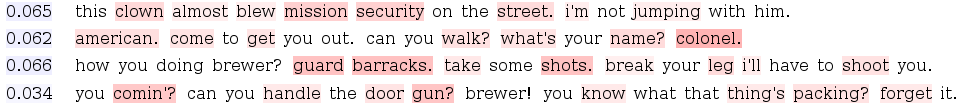
\includegraphics[scale=0.43]{pics/military.png}
   \caption{\textit{profession}: military personnel}
   \label{fig:att-profession}
 \end{subfigure}
 \\[8pt]
 \begin{subfigure}{.9\textwidth}
   \centering
   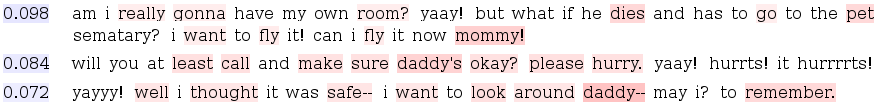
\includegraphics[scale=0.43]{pics/child.png}
   \caption{\textit{age} (category): child}
   \label{fig:att-age}
 \end{subfigure}
\vspace*{-0.3cm}
\caption{Attention visualization for \textit{profession} and \textit{age} attributes on MovieChAtt.}
\label{fig:att-profession-age}
\end{figure*}

\begin{figure*}[th!]
 \centering
 \begin{subfigure}{.9\textwidth}
   \centering
   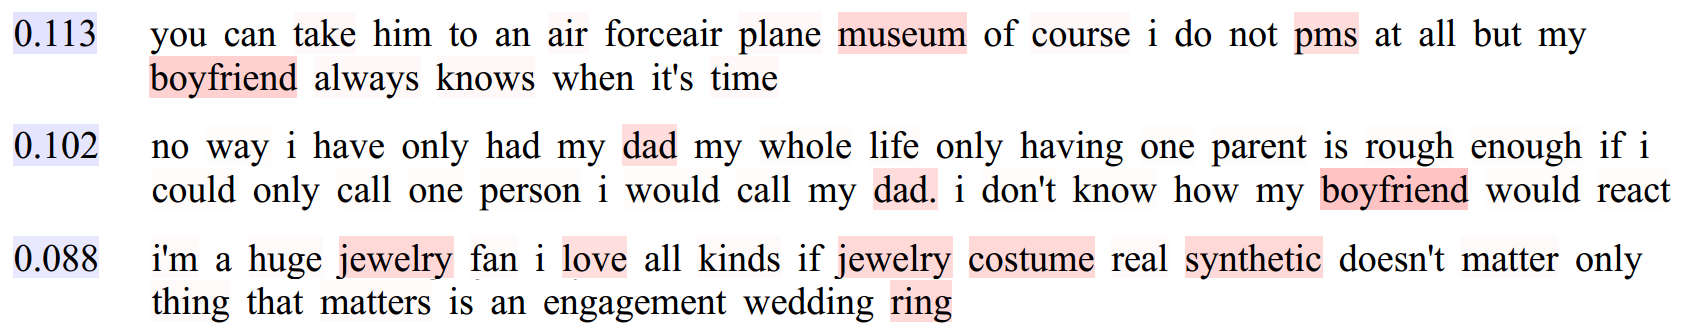
\includegraphics[scale=0.17]{pics/gender_att.png}
   \caption{\textit{gender}: female}
   \label{fig:att-gender}
 \end{subfigure}
 \\[8pt]
 \begin{subfigure}{.9\textwidth}
   \centering
   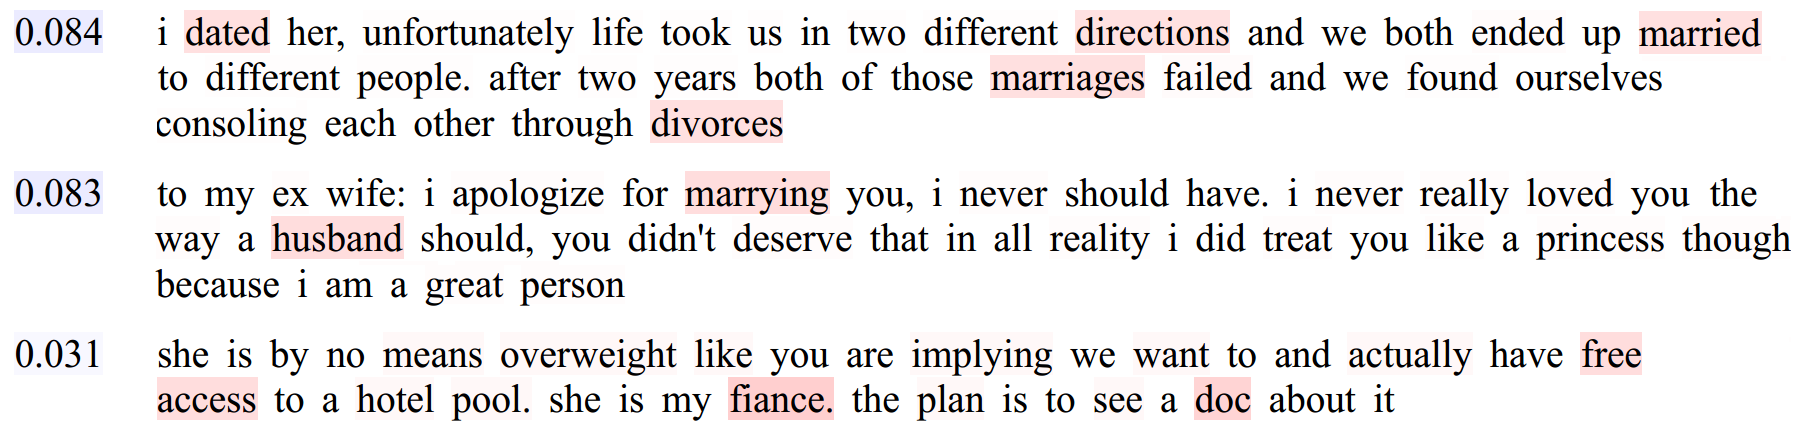
\includegraphics[scale=0.17]{pics/family_att.png}
   \caption{\textit{family status}: married}
   \label{fig:att-family}
 \end{subfigure}
\vspace*{-0.3cm}
\caption{Attention visualization for \textit{gender} and \textit{family status} attributes on RedDust.}
\label{fig:att-gender-family}
\end{figure*}


\subsection{Case study on attention weights}

In order to illustrate the types of terms the models are looking for, we display \method{2attn}'s term and utterance weights for 
\textit{profession} and \textit{age} attributes (on the MovieChAtt dataset) in Figure \ref{fig:att-profession-age}, as well as \textit{gender} and \textit{family status} attributes (on RedDust) in Figure \ref{fig:att-gender-family}.
While \method{2attn} is 
%sometimes
often outperformed by \method{CNN-attn}, this model is more interpretable because individual terms are considered in isolation.
%Note that all these dialogue snippets come from the specific
%datasets in our experiments, partly from fictional
%conversations.
%Some are skewed and biased, and not representative
%for the envisioned downstream applications.

When predicting \textit{military personnel} as the \textit{profession} (Figure \ref{fig:att-profession}), the model focuses on military terms such as \textit{mission}, \textit{guard}, \textit{barracks}, and \textit{colonel}.
When predicting \textit{child} as the \textit{age category} (Figure \ref{fig:att-age}), on the other hand, the model focuses on terms a child is likely to use, such as \textit{pet}, \textit{mommy}, and \textit{daddy}.
According to Reddit posts, \textit{female} gender is suggested by terms such as \textit{boyfriend}, \textit{pms} and \textit{jewelry} (Figure \ref{fig:att-gender}). Meanwhile, \textit{married} users were identified through terms such as \textit{dated}, \textit{fiance} and \textit{divorces}, along with obvious terms like \textit{marrying} and \textit{marriages} (Figure \ref{fig:att-family}). 
These examples illustrate how the model is able to infer a speaker's attribute by aggregating signals across utterances.

In addition to looking at specific utterances, we investigated which terms the model is strongly associating with a specific attribute. To do so, we computed attribute value probabilities for each term in the corpus, and kept the top terms for each attribute value. The results using \method{2attn} are shown in Table \ref{tab6}, which is divided into words that appear informative (top section) and words that do not (bottom section). In the case of informative words, there is a clear relationship between the words and the corresponding profession. 
Many of the uninformative words appear to be movie-specific, such as names (e.g., xavier, leonard) and terms related to a \textit{waiter's} role in a specific movie (e.g., rape, stalkers). Reducing the impact of setting-specific signals like this is one direction for future work.

\begin{table}[t]
\centering
\small
%\begin{adjustbox}{width=0.475\textwidth,center}
\begin{tabular}{@{}l@{\hskip 0.5\tabcolsep}l@{}}
\toprule
\textbf{profession} & \textbf{significant words} \\
\midrule
\textit{scientist} & characteristics, theory, mathematical, species, changes \\
\textit{politician} & governors, senate, secretary, reporters, president \\
\textit{detective} & motel, spotted, van, suitcase, parked \\
\textit{military personnel} & captured, firepower, guard, soldiers, attack \\
\midrule
\textit{student} & playing, really, emotional, definitely, unbelievable \\
\textit{photographer} & xavier, leonard, collins, cockatoo, burke \\
\textit{waiter} & rape, stalkers, murdered, overheard, bothering \\
\bottomrule
\end{tabular}
%\end{adjustbox}
\caption{Top-5 words from \method{2attn} characterizing each profession.
}
\label{tab6}
\end{table}

\vspace{-5pt}
\subsection{Insights on transfer learning}

To investigate the robustness of our trained HAMs,
we tested the best performing models (i.e., \method{2attn} and \method{CNN-attn})
on a transfer learning task between our datasets. 
Specifically, we leveraged user-generated social media text (RedDust posts) available in abundance to train the models and subsequently performing inference on the speech-based dialogues (MovieChAtt and PersonaChat). 
We report the results in Tables \ref{tab:transfer-learning-reddit-moviechatt} and \ref{tab:transfer-learning-reddit-personachat} respectively.

While the scores on PersonaChat are low compared to those in Tables \ref{tab:model-comparison-gender}, \ref{tab:model-comparison-profession} and \ref{tab:model-comparison-family}, the HAMs' performance on MovieChAtt is often comparable with the baselines' performance in Tables \ref{tab:model-comparison-gender}, \ref{tab:model-comparison-profession}, \ref{tab:model-comparison-age} and \ref{tab:model-comparison-family}.
This difference may be caused by the fact that PersonaChat is a smaller, more synthetic dataset, as discussed in Section \ref{findings}.

On MovieChAtt with the \textit{profession} attribute, both HAMs match the performance of all six baselines in terms of macro MRR. Similarly, \method{2attn} matches the performance of five of the six baselines on the \textit{gender} attribute (accuracy), and \method{CNN-attn} matches the performance of four of the six baselines on the \textit{age} attribute (macro MRR). The methods do not perform as well in terms of micro MRR, which may be due to the substantially different attribute value distributions between datasets.
Particularly for the \textit{profession} attribute, the lower performance can be explained by missing training instances  for certain professions in the RedDust dataset, such as \textit{astronaut} or \textit{monarch}. 
Improving HAMs' transfer learning performance is a direction for future work.


\begin{table}[t]
\centering
\small
\begin{adjustbox}{width=0.9\textwidth,center}
\begin{tabular}{@{}lc@{}cc@{\hskip 1\tabcolsep}cc@{}c@{}}
\toprule
\multirow{3}{*}{\textbf{Models}} & \multicolumn{2}{c}{\textbf{profession}\vspace{3pt}} & \multicolumn{2}{c}{\textbf{gender}} & \multicolumn{2}{c}{\textbf{age}} \\
\cmidrule(lr){2-3} \cmidrule(lr){4-5} \cmidrule(lr){6-7}
 & \multicolumn{1}{c}{MRR} & \multicolumn{1}{c}{\multirow{2}{*}{AUROC}} & \multicolumn{1}{c}{\multirow{2}{*}{Acc}} & \multicolumn{1}{c}{\multirow{2}{*}{AUROC}}  & \multicolumn{1}{c}{MRR} & \multicolumn{1}{c}{\multirow{2}{*}{AUROC}}  \\
 & \multicolumn{1}{c}{micro / macro} & &  & & \multicolumn{1}{c}{micro / macro} & \\
\midrule
\Tstrut \method{CNN-attn}     & 0.19 / 0.18 & 0.58 & 0.56 & 0.58 & \textbf{0.57} / \textbf{0.54} & \textbf{0.69} \\ 
\method{2attn}                & \textbf{0.21} / \textbf{0.21} & \textbf{0.67} & \textbf{0.61} & \textbf{0.64} & 0.45 / 0.41 & 0.45 \\
\bottomrule
\end{tabular}
\end{adjustbox}
\caption{Transfer learning performance of pre-trained RedDust models on MovieChAtt.}
\label{tab:transfer-learning-reddit-moviechatt}
\end{table}



\begin{table}[t]
\centering
\small
%\begin{adjustbox}{width=0.475\textwidth,center}
\begin{tabular}{@{}lcccccc@{}}
\toprule
\multirow{3}{*}{\textbf{Models}} & \multicolumn{2}{c}{\textbf{profession}\vspace{3pt}} & \multicolumn{2}{c}{\textbf{gender}} & \multicolumn{2}{c}{\textbf{family status}} \\
\cmidrule(lr){2-3} \cmidrule(lr){4-5} \cmidrule(lr){6-7} 
 & \multicolumn{1}{c}{MRR} & \multicolumn{1}{c}{\multirow{2}{*}{AUROC}} & \multicolumn{1}{c}{\multirow{2}{*}{Acc}} & \multicolumn{1}{c}{\multirow{2}{*}{AUROC}}  & \multicolumn{1}{c}{\multirow{2}{*}{Acc}} & \multicolumn{1}{c}{\multirow{2}{*}{AUROC}} \\
 & \multicolumn{1}{c}{micro / macro} &  &  &  &  & \\
\midrule
\Tstrut \method{CNN-attn}     & 0.20 / 0.16 & 0.58 & \textbf{0.52} & 0.50 & \textbf{0.74} & \textbf{0.74} \\
\method{2attn}                & \textbf{0.21} / \textbf{0.18} & \textbf{0.71} & 0.51 & \textbf{0.54} & 0.62 & 0.64 \\
\bottomrule
\end{tabular}
%\end{adjustbox}
\caption{Transfer learning performance of pre-trained RedDust models on PersonaChat.}
\label{tab:transfer-learning-reddit-personachat}
\end{table}

\subsection{Profession misclassification study}
In this section we investigate common misclassifications on the MovieChAtt dataset for the \textit{profession} attribute, which is the most challenging attribute with the most possible values.
A confusion matrix for \method{2attn} is shown in Figure \ref{matrix}.
Dotted lines indicate several
interesting misclassifications: \textit{policemen} are often confused with \textit{detectives} and \textit{special agents} (red line); \textit{scientists} are confused with \textit{astronauts} (yellow line), because sci-fi films often feature characters who arguably serve in both roles; and a \textit{child} is often labeled as a \textit{student} or a \textit{housewife} (green line) because they sometimes use similar terms (e.g., `school' is used by both children and students, and `mommy' is used by both children and housewives).
Finally, 
many occupations are confused with \textit{criminal}, which is the most common profession in MovieChAtt.


\begin{figure}[t]
\centering
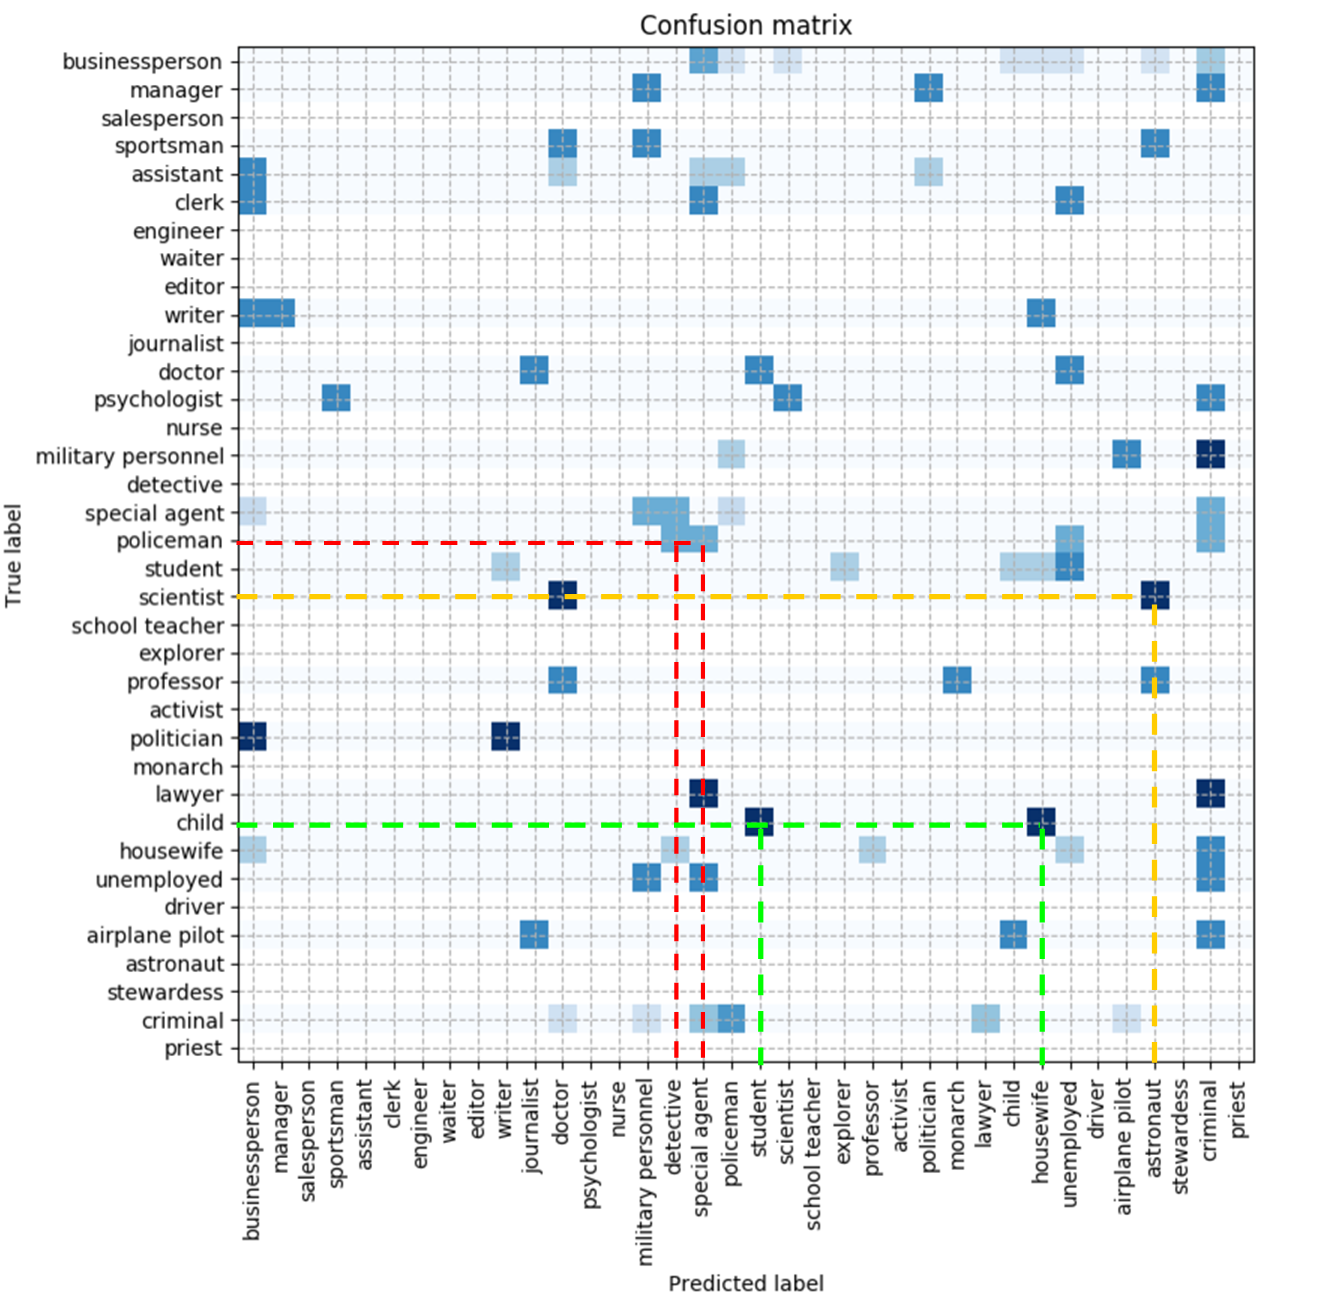
\includegraphics[width=0.7\textwidth]{pics/conf_new.png}
\vspace*{-0.3cm}
\caption{Confusion matrix computed with \method{2attn}. True positives are not shown. Darker squares indicate more misclassifications.}
\label{matrix}
\end{figure}



%%%%%
% Transfer learning confusion matrix (was in original HAM paper)
%
%To further compare the performance of the model on direct and transfer learning tasks we computed the confusion matrix for \method{2attn} trained on the Reddit dataset and using MovieChAtt as the test corpus. Interesting misclassifications include the following: artistic professions (\textit{actor}, \textit{painter}, \textit{musician}, \textit{director}) are often mixed up (red lines); \textit{banker} is confused with \textit{manager} (green lines); \textit{policeman} and \textit{airplane pilot} are confused with \textit{military personnel} (purple lines); and \textit{stewardess} is often confused with \textit{nurse} as they both are related to caring and serving tasks (yellow line).

%\begin{figure}[t]
%\centering
%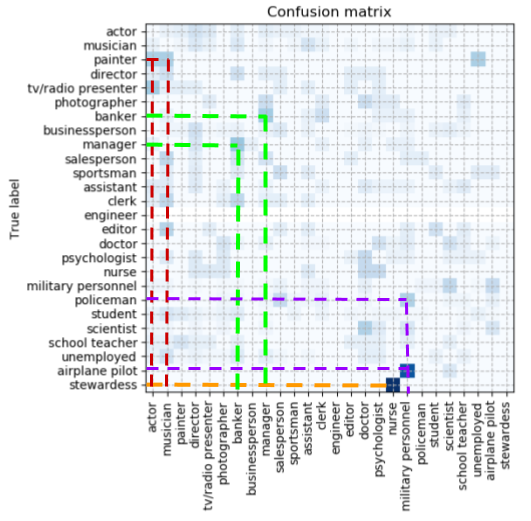
\includegraphics[width=0.75\textwidth]{pics/conf_transfer_crop.png}
%\vspace*{-0.3cm}
%\caption{Confusion matrix of Reddit$_{\text{train}}$ $\rightarrow$ %MovieChAtt$_{\text{test}}$ computed with \method{2attn}. True positives are not shown. %Darker squares indicate more misclassifications.}
%\label{matrix-reddit}
%\end{figure}


\section{Conclusion}
In this chapter we proposed Hidden Attribute Models (HAMs) for inferring personal attributes from conversations, such as a person's profession. 
We demonstrated the viability of our approach in extensive experiments considering several attributes on three datasets with diverse characteristics: Reddit discussions, movie script dialogues and crowdsourced conversations. 
Furthermore, we used an oracle approach to demonstrate that pattern matching is insufficient for extracting personal attributes from conversations, because such attributes are rarely explicitly mentioned.
We compared HAMs against a variety of state-of-the-art baselines, showing that HAMs achieve
substantial improvements over all of them.%, most notably by the \method{CNN-attn}
%and \method{2attn} variants. 
We also demonstrated that the attention weights assigned by our methods provide
informative explanations of the computed output labels.

As a stress test for our methods, we investigated transfer learning by
training HAMs on one dataset and applying the learned models to other datasets.
Although we observed degradation in output quality, compared to
training on in-domain data, it is noteworthy that the transferred HAMs
matched the performance of the baselines when trained on in-domain data.
%We plan to further investigate this theme of transfer learning in our future work
%on construction personal knowledge bases and leveraging them for personalized Web agents.

\subsection{Limitations and future work}

In this section we enumerate possible directions for future work, some of which are motivated by the limitations of the approach proposed in this chapter.

\begin{itemize}
    \item \textbf{Limited attribute value lists.} Many personal attributes, such as \textit{hobby} or \textit{profession}, have long lists of possible values. In our experiments on predicting professions with HAMs we carefully selected the most popular occupations, which have sufficient amount of labeled examples. This approach misses out on many rare attribute values, for which the training examples are scarce or even not available. Moreover, a significant amount of human supervision is required to manually refine the attribute value lists. In the next chapter we propose our solution to this issue.
    
    \item \textbf{Improved transfer learning.} Our experiments with HAMs were based on the assumption that the input data resembles actual conversations. However, this is far from being true: the dialogues in MovieChAtt are based on fictional events and sound metaphorical, PersonaChat conversations are artificial and very short, discussion threads in RedDust are distinct from face-to-face offline dialogues. Therefore, there is a genuine need to devise new models having strong transfer learning abilities, so that the method trained on the richly annotated artificial datasets would be able to make proper inference on real-life conversations. %Although our experiments have shown that HAMs can to some extend perform transfer learning, it could still be further enhanced. 
    
    \item \textbf{Combined prediction of several attribute values.} Most personal attributes are interdependent (e.g. a 6 year old person can't be a manager or be married). Thus the method for predicting personal attributes should ultimately leverage the relationships between multiple attributes by extracting them with a single model. This facilitates the extension of the architecture to any new personal attribute of interest and saves computational resources for training separate models for each attribute.
    
\end{itemize}



\chapter{Conversational Hidden Attribute Retrieval Model}
\label{chap_charm}
\minitoc
\droppedcapital{P}ersonal knowledge about users' professions, hobbies, favorite food, and travel preferences, among others,
is a valuable asset for individualized AI, such as
recommenders or chatbots.
Conversations in social media are
a rich source of data for inferring 
%this kind of 
personal facts.
Prior work developed supervised %attribute 
methods to extract this knowledge, 
but these approaches
can not generalize beyond 
attribute values 
%that were seen as training labels.
with ample labeled training samples. 
Such models are thus inapplicable for the \textit{long-tailed} personal attributes, such as \textit{hobby}, when there is little chance of acquiring labeled training data for rare values.
We overcome
this limitation
by devising CHARM: a
zero-shot learning
method 
%based on reinforcement learning, 
that creatively leverages keyword extraction and document retrieval
in order to
predict attribute values 
that were never seen during training.
Experiments with 
large datasets from Reddit
show the viability of CHARM
for open-ended attributes, such as professions
and hobbies.

\section{Introduction}

\paragraphHdTop{Motivation.} Personal Knowledge Bases 
capture user traits
for %personalizing 
customizing
downstream applications like chatbots
or recommender systems \cite{Balog:2019:TSE:3331184.3331211}.
To provide recommendations that are tailored to the fine-grained characteristics and interests of the user, a PKB should contain personal attributes with a wide range of possible values, such as hobbies, professions, cities visited, medical conditions 
(experienced by the user) and many more.

A potentially automatic way to populate a PKB with such attributes is to 
draw them from the user's conversations in social media and dialogues on other platforms. However, a large number of personal attributes 
and their respective values makes this a challenging task. In particular, there is little hope to have training data for each of these key-value pairs.
Moreover, the textual cues in user conversations are often implicit
and thus difficult to learn.

\paragraphHd{Example.}
Consider the user's utterance:
\textit{``I just visited London, which was a disaster. My hotel was a headache and I spent half the time in bed with a fever... So glad to be back home finishing the masts on my galleon.''}

As humans, we can infer the following attribute-value pairs: 
(a) \textit{cities visited:London}, (b) \textit{symptom:fever},
(c) \textit{hobby:model ships}. 
However, with both implicit and explicit signals present capturing such user traits is a daunting task.
We need to consider the context \textit{``spent in bed with''}, to infer that \textit{fever} relates to a disease (as opposed to \textit{headache}). 
To predict the user's hobby \textit{model ships}, we have to pay attention to the cues `\textit{galleon}' and `\textit{mast}'.
Proper inference requires both deep language understanding and background knowledge
(e.g., about ships, cities,
etc.).

\vspace{0.1cm}
\paragraphHd{State of the Art and its Limitations.}
Explicit mentions of attribute-value pairs can be captured by pattern-based methods (e.g., \cite{dial7,Yen:2019:PKB:3331184.3331209}).
Such methods are able to extract `\textit{London}' 
from the the previous example by using the pattern \textit{``I \dots visited $\langle$city\_name$\rangle$}''.  
Pattern-based approaches are limited, though, by
their inability to consider implicit contexts, such as %{\em `in bed with \dots}'.
{\em ``finishing the \textbf{masts} on my \textbf{galleon}''}. 
Question answering methods can be used to relax rigid patterns 
(e.g., \cite{levy2017zero}), 
but still rely on explicit mentions of attribute values.

In this work we 
aim to extract
attribute values leveraging both explicit and implicit cues, such as inferring \textit{symptom:fever} and \textit{hobby:model ships}.
Additionally, we address the cases where there is a long-tailed set of
values for such attributes as {\em hobby}. 
In principle, deep learning is suitable for such inference \cite{tigunova:ham:2019, pietro:ACL15, Rao:2010}, but it critically hinges on the availability of labeled
training samples for \text{every attribute value} 
that the model should predict.

Supervised training is suitable for a pre-specified limited-scope setting, such as learning
personal interest from a fixed list of ten movie genres, but it does not
work for the situation with large and open-ended sets of possible values,
for which there is little hope of obtaining comprehensive training samples.
Therefore, we pursue a {\em zero-shot learning} \cite{larochelle2008zero, palatucci2009zero} 
approach that learns from
labeled samples for a small subset of labels (i.e., attribute values in our
setting) and generalizes to the full set of labels including values {\em unseen}
at training time.

\paragraphHd{Problem Statement.}
For a given attribute we consider the set of \emph{known} values $V$, which can be drawn from lists in dictionary-like sources, such as Wikipedia. 
At training time, our method requires samples for a small 
subset of values $S \subset V$.
Typically, the complement $V \setminus S$
is much larger than $S$: $|V \setminus S| \gg |S|$.
For instance, $S$ may consist solely
of the popular values \emph{sports, travel,
reading, music, games}, whereas the complement
includes hundreds of long-tail values, such as
\emph{beach volleyball}, \emph{model ships}, \emph{brewing}, etc.
At inference time
we need to predict values from
all of $V$, although most of the values are \textit{unseen} during training.

\vspace{0.1cm}
\paragraphHd{Approach and Contributions.}
We present a 
\textbf{C}onversational 
\textbf{H}idden 
\textbf{A}ttribute 
\textbf{R}etrieval 
\textbf{M}odel (CHARM) for inferring attribute values in a zero-shot setting \cite{tigunova2020charm}.
CHARM identifies cues in related to a target attribute, which it then uses to retrieve relevant texts from external document collections, indicative of different attribute values.
These external documents could be gathered by simple web search.
They help CHARM to link the cues in the user's utterances 
to the actual attribute values to predict.

CHARM consists of two components: \emph{(i)} a \textit{cue detector}, which identifies attribute-relevant keywords in a user's utterances 
(e.g., `\textit{galleon}'), and \emph{(ii)} a \textit{value ranker}, which matches these keywords against documents that indicate possible values of the attribute (e.g., \textit{model ships}). 
Attribute values predicted by CHARM must be \textit{known} but CHARM does not require all values to be \textit{seen} during training. 

To evaluate our approach, we conduct experiments predicting Reddit users' professions and hobbies based on their conversational utterances. We demonstrate that CHARM performs well when inferring unseen values and performs competitively with the best-performing baselines when 
predicting values seen during training. 
CHARM can easily be extended to other attributes with long-tail values, such as 
{\em favorite cuisine}, {\em preferred news topics} or {\em medication taken}, by providing a list of known attribute values, training examples for a subset of these values and access to external documents (e.g., via a Web search engine).

\vspace{0.1cm}
The salient contributions of this work are:
%\vspace{0.2cm}
%\begin{itemize}
\squishlist
    \item a method for inferring both seen and previously unseen (zero-shot) attribute values from a user's conversational utterances;
    \item a comprehensive evaluation 
    for the \textit{profession} and \textit{hobby} attributes over a large dataset of Reddit discussions;
and \item a demonstration platform\footnote{\href{https://d5demos.mpi-inf.mpg.de/charm}{https://d5demos.mpi-inf.mpg.de/charm}} showcasing the ability of CHARM to make predictions from dialogue with the user or the user's social media submissions \cite{tigunova2021exploring}.
\squishend
%\end{itemize}


\section{Related work}

\paragraphHd{Zero-shot learning.}
CHARM 
is designed for handling attribute values
that were never seen at training time -- a \emph{zero-shot learning} problem, extensively studied in the field of computer vision but less explored in NLP. A technique employed in CHARM is similar to the approach proposed by \citet{zero-shot15} for visual classes, which
builds image classifiers directly from
encyclopedia articles  
without
training images.

Most zero-shot studies for NLP \cite{wang2019survey} deal with machine translation, cross-lingual retrieval and entity/relation extraction. For example, in \textit{relation extraction} task \cite{levy2017zero} the relations serve as unseen classes and their instances are recovered by casting the relations to natural language questions and reducing the problem to reading comprehension; in \textit{entity extraction} \cite{pasupat2014zero} the extraction of entities from the web documents is done with a text query, removing the need for specifying a set of seed terms. Methods proposed in \cite{levy2017zero, pasupat2014zero} are not suitable for our task, because they identify values that are explicitly mentioned, rather than inferring them. Our task is similar to zero-shot \textit{text classification} \cite{yazdani2015model, zhang2019integrating}, where the class labels are represented as single-word embeddings.

Other zero-shot models solving natural language problems include the ones for text filtering and classification. \citet{li2018deep} solve the task of zero-shot \textit{document filtering} by learning relevance between categories and documents, which are represented with category-dependent embeddings. \citet{dauphin2013zero} investigates zero-shot \textit{semantic utterance classification}, by mapping the utterances and potentially unseen categories into same semantic space, where they can be matched with distance functions.

\paragraphHd{Keyword extraction from conversational text.} 
Keyword or keyphrase extraction concerns the task of automatic selection of important terms from a document that best represent its content. The extracted terms are beneficial for many applications including document indexing, summarization and classification. 

Owing to its importance, several extraction methods have been extensively studied and evaluated on various corpora, mostly on news articles, web documents and scientific/technical reports. Less attention has been given to keyword extraction from conversational texts, such as meeting transcripts \cite{liu-etal-2009-unsupervised,7045531}, live chats \cite{kim-baldwin-2012-extracting} and social media posts \cite{Zhao:2011:TKE:2002472.2002521,wu-etal-2010-automatic-generation,zhang-etal-2016-keyphrase}.
Notable applications of keyword extraction from conversations include 
%with continuous monitoring of users' activities,
generating personalized tags for Twitter users \cite{wu-etal-2010-automatic-generation}, searching for relevant email attachments \cite{van2017reply} and just-in-time information retrieval \cite{7045531}.

Prior work 
mostly
pursued unsupervised keyword extraction approaches \cite{mihalcea2004textrank, rose2010automatic},
due to limited availability of
training data. Few studies use supervised learning, with feature-based classifiers \cite{kim-baldwin-2012-extracting} 
or neural sequence tagging models \cite{zhang-etal-2016-keyphrase}. 
Our neural approach for keyword detection 
lies in between, as we 
learn to identify 
salient keywords for a specific attribute (e.g., \emph{profession}),
without having training data of relevant keywords.

Unsupervised techniques for keyword extraction can generally be split into several categories \cite{hasan-ng-2014-automatic}, notably: \textit{(i)} \textit{statictical}, which are based on simple word features, such as term frequency or relational position in the document \cite{ramos2003using, campos2018yake}, word co-occurrence \cite{matsuo2004keyword} or keyphrase co-occurrence counts \cite{rose2010automatic}; and \textit{(ii)} \textit{graph-based}, which utilize a word/phrase graph constructed from the document and extract keywords using graph ranking methods \cite{mihalcea2004textrank, bougouin:hal-00917969}. We consider two unsupervised keyword extraction architectures as baselines: statistical method \textit{RAKE} \cite{rose2010automatic} and graph-based model \textit{TextRank} \cite{mihalcea2004textrank}.


\paragraphHd{Information Retrieval in NLP.} 
Most existing work leveraging information retrieval components to solve NLP tasks focused on question answering  %\cite{kratzwald-feuerriegel-2018-adaptive,Cui:2005:QAP:1076034.1076103,Yang:2016:ARS:2983323.2983818,chen2017reading,wang2018r,yang2019end}
\cite{kratzwald-feuerriegel-2018-adaptive,wang2018r, guu2020realm}
% removed these to shorten list: Zhu:2019:HAR:3308558.3313699,surdeanu-etal-2008-learning,
or dialogue systems 
%\cite{feng-etal-2019-learning,Tao:2019:MFN:3289600.3290985,Luo2019Personalized,dial4}. 
\cite{feng-etal-2019-learning,Luo2019Personalized},
%\textcolor{red}{The study \cite{guu2020realm} uses retrieval-based pretraing for the QA-model.}
where the retrieval part is responsible for ranking the most appropriate answers or responses, given a question or chat session. As far as we know, we are the first to leverage a retrieval-based 
model for inferring 
attribute values without training samples.

\paragraphHd{Reinforcement Learning in NLP.}
Reinforcement learning (RL) methods are often applied in conversational models for response generation \cite{kandasamy2017batch}, based on the feedback from human quality assessment scores for the output utterances. Other NLP tasks where reinforcement learning can be applied include question answering \cite{qu2019learning, liu2020knowledge}, text classification \cite{zhang2018learning} and entity linking \cite{fang2019joint}. 

Several studies use RL decision processes to pick up relevant words or phrases from the input texts, which is close to our work. For example, \citet{wang2019aspect} proposed to perform aspect-level sentiment classification using reinforcement learning to select segments of texts on which the sentiment should be predicted. \citet{chen2018joint} detects events and their corresponding keywords from Twitter texts using an RL method to select posts, which talk about events and extract keywords from them. \citet{zhang2018learning} proposed a reinforcement learning agent that selects the words which should be removed from the sentences, creating a concise sequence representation. %The created concise sentence representation is used in classification task, the performance in which acts as a reward signal for the agent.



\section{Background}

Training CHARM involves applying a non-differentiable \texttt{argmax} operation, which prevents using end-to-end backpropagation. In this section we provide the technical background on the \textit{policy gradient method}, which we use to mitigate this problem.

\textit{Reinforcement learning} is a machine learning technique based on training an intelligent agent to maximize the reward by selecting appropriate actions. The agent interacts with the \textit{environment} by observing its current state and taking actions; as a result the agent gets the feedback from the environment, which serves as a signal about the correctness of the chosen action. Reinforcement learning environment can be formulated as a \textit{Markov Decision Process}, a tuple $(S, A, P, r, \gamma)$, where 
\squishlist
    \item $S$ is a finite set of states,
    \item $A$ is a finite set of actions,
    \item $T(s,a) = s' : S \times A \rightarrow S$ is the \textit{transition function}, specifying the mapping from the current state $s$ and the taken action $a$ to a new state $s'$,
    \item $r(s,a) : S \times A \rightarrow \mathbb{R}$ is the \textit{reward function}, specifying the real-valued reward for taking the action $a$ while being in state $s$,
    \item $\gamma \in (0,1]$ is the discounting factor, representing the decrease of the reward for the actions further in the future.
\squishend

A stochastic \textit{policy} $\pi(a_t| s_t)$ is a function, specifying the probability of taking action $a_t$ while being in the state $s_t$ at the timestep $t$. A \textit{trajectory} $\tau = [s_t, a_t]_{t=0}^T$ is a sequence of (state, action) steps, induced by the policy $\pi$, where $T$ denotes the terminal step. The \textit{expected  reward} $J$ is defined as:

\begin{equation}
    J(\theta) = \mathbb{E}_{\tau \sim p_{\pi}(\tau)} \sum_{t=0}^{T} \gamma^t r(s_t, a_t| \pi)
\end{equation}

where the expectation is computed with respect to possible random trajectories $\tau \sim p_{\pi}(\tau)$, determined by the policy function. The expected reward defines the mathematical expectation of the total gain until timestep $T$ by following the policy $\pi$.

\textit{Policy gradient methods} solve reinforcement learning problems, which have parameterized differentiable policy function $\pi_{\theta}$, by maximizing the expected reward  $J(\theta)$ with respect to $\theta$. This is done by differentiating $J(\theta)$ using the following formula:

\begin{equation}
    \triangledown_{\theta} J(\theta) = \sum_{t=1}^K R_t \triangledown_{\theta} log \pi_{\theta} (a_t|s_t)
\end{equation}

where $R_t$ is the discounted future cumulative reward:

\begin{equation}
    R_t = \sum^T_{t' = t + 1}\gamma^{t'-t-1}r_{t'}
\end{equation}

The policy $\pi$ could be implemented by a neural network, which parameters $\theta$ are to be updated using policy gradient methods. For example, this can be done with the REINFORCE algorithm \cite{williams1992simple}. In REINFORCE the reinforcement learning agent generates a random trajectory under the current policy $\pi_{\theta}$ and then, for every timestep in the trajectory $t = 1$ to $T$, the policy parameters are updated as follows:

\begin{equation}
    \theta_{new} = \theta_{old} + \alpha \triangledown_{\theta} R_t log \pi_{\theta} (a_t|s_t)   
\end{equation}
\section{Methodology}

In this section we describe CHARM, our proposed model for inferring personal attributes from conversations. As illustrated in Figure \ref{pipeline}, CHARM's operation consists of two stages: \emph{cue detection} and \emph{value ranking}. 
As input CHARM receives the user's utterances $U=u_0..u_N$ that contain a set of terms $t_0..t_M$, for example, $U=${\em 
\{``I stayed late at the \textbf{library} yesterday'', ``\textbf{Studied} for the \textbf{exam} so I could have better \textbf{grades} than my \textbf{classmates}''}\}. 
In the first stage, the term scoring model assigns a score to each term in the user's utterances, yielding $l_0..l_M$. The highest scoring terms are then selected to form a query $Q=q_0..q_K$, characterizing the user's correct attribute value, e.g., $Q=$``library studied exam grades classmates'' for the \emph{profession} attribute. 

In the second stage, $Q$ is evaluated against an external document collection $D=d_0..d_L$; each document in $D$ is associated with possible attribute values.  
Documents such as \emph{Wiki:Student} and \emph{Wiki:Dean's List}
\footnote{Wikipedia pages: \href{https://en.wikipedia.org/wiki/Student}{{Student}} \& \href{https://en.wikipedia.org/wiki/Dean\%27s_list}{{Dean's\_list}}}, which are associated with the attribute value \emph{student}, would score high with the example query.
The score aggregator then ranks the attribute values based on the documents' scores $s_0..s_L$, for instance, yielding a high attribute score for \emph{student} given our example utterances. The list of attribute values $V$ is \textbf{known} in advance (e.g., taken from Wikipedia list of professions); however, potentially only a subset of values $S \subset V$ have instances \textbf{seen} during training.


\begin{figure}[t!]
\centering
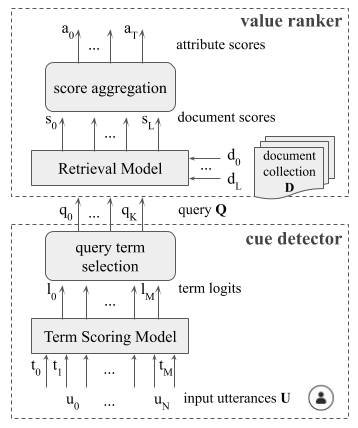
\includegraphics[width=0.45\textwidth]{imgs/scheme.png}
\vspace*{-0.3cm}
\caption[The pipeline of CHARM.]{The pipeline of CHARM.
The Term Scoring Model assigns scores $l_0 .. l_M$ to the terms in the input utterances $u_0..u_N$. The terms with the highest scores are passed to the Retrieval Model, which queries the document collection $D$. The document scores are aggregated to produce attribute value scores
for predictions.
}
\label{pipeline}
\end{figure}

The rank of the correct attribute value acts as a distant supervision signal, allowing us to train term selection, regardless of the non-differentiable \texttt{argmax} operation.
CHARM is trained using reinforcement learning via the REINFORCE policy gradient method described in the previous section.


\subsection{Cue detection}
\label{sec:term-selection}

The  term scoring model $\delta$ evaluates how useful
each word in a given user's utterances is for making a prediction,
and assigns real-value scores $l_0 ... l_M$ to the terms accordingly. 
That is,
    $l_j = \delta (t_j | t_0, .. t_M; W)$,
where $W$ denotes the parameters of the model. The term scores $l_0 .. l_M$ are then used to select the words which will form the query for the value ranking component. 

Due to our use of REINFORCE, the selection process differs between the training and prediction settings.
During training, the scores $l_0 .. l_M$ are normalized with a softmax function to obtain
probabilities $p_0 ... p_M$, which are used to incrementally sample without replacement a query consisting of $K$ terms. The query length $K$ is a hyperparameter, optimized in the grid search.
The sampling in effect allows the words with low scores a better chance to be selected,
thus encouraging exploration. At inference time the query is formed by taking the terms with $K$ top scores.
%In our example, the word `library' will have a greater probability to be sampled during training time, %and 
%will only be selected during test time if its score is high enough to get into the top $K$ terms.

The term scoring model 
should produce high scores for terms that are descriptive of the user and of the attribute in general, instead of a specific attribute value. This means that it should be able to exploit background knowledge and a term's context to 
judge its relevance to the attribute.
For instance, having seen the phrase \emph{``stayed late at the hospital''} for the 
\emph{physician} at training time, at prediction time an ideal model would correctly estimate the importance of the word `\textit{library}' in the phrase \emph{``stayed late at the library''}, even if there were no instances of \emph{student} in the training set. Considering this, we give preference to the models that operate on sequences, as opposed to the bag-of-word models. We select BERT \cite{devlin2018bert} as our term scoring model, because it is a sequential model incorporating world knowledge that should effectively use word context, predicting whether terms are related to an attribute.

For further description, let us suppose the cue detector picks the words $Q = q_0 ... q_K$ as the query terms for CHARM's value ranking stage. A typical query would consist of the terms associated with the correct attribute value (for example, $Q=$``\textit{library studied exam grades classmates}'').

\subsection{Value ranking}
The second stage of the model consists of two steps: first, using the selected query terms to rank the documents in the external collection; and second, aggregating document scores to predict values.

\paragraph{Document ranking.}
The ranking component takes two inputs: query terms $Q = q_0 ... q_K$ resulting from the cue detector and an (automatically labeled) document collection $D = d_0 ... d_L$.
% \squishlist
%     \item query terms $Q = q_0 ... q_K$, resulting from the previous step and
%     \item the (automatically labeled) document collection $D = d_0 ... d_L$ of the size $L$.
% \squishend
The document collection
could be a set
of Web pages, where each page indicates a specific attribute value, $v_0 ... v_L$. 
For example, by 
generating a search-engine query ``\textit{hobby $\langle$value$\rangle$}'' we can gather 
web pages related to specific hobbies. 

The ranker $\rho (Q, d_k)$ evaluates the query $Q$,
constructed by the cue detector,
against each document $d_k$ in the document collection to produce document relevance scores $s_0 ... s_L$. For the example query ``\textit{library studied exam grades classmates}s'', the document \emph{Wiki:Dean's List} labeled with \emph{student} will get a higher score than \emph{Wiki:Junior doctor} (for \emph{physician}). 

We consider two particular instantiations of the ranker:
BM25 \cite{robertson1995okapi} and KNRM \cite{xiong2017end}, described in Chapter \ref{back_ir}.
BM25 is a strong unsupervised retrieval model, whereas KNRM is an efficient neural retrieval model that can consider semantic similarity via term embeddings in addition to considering exact matches of query terms. 
%The ranker can also be instantiated by any existing IR model.

\paragraph{Document score aggregation.}
The document scores $s_0 ... s_L$ obtained from the ranker are then aggregated to produce scores for each known attribute value. 
Depending on the document collection used, each attribute value may be represented by several documents. For example, the \textit{student} attribute value may be associated with documents \emph{Wiki:Dean's List}, \emph{Wiki:Master's degree}, etc.  In this case, the scores per document have to be aggregated to form the final scores $a_0 ... a_T$ for each attribute value in $V$. In our experiments, we consider the following aggregation techniques: \emph{(i)} \emph{average} (which allows multiple documents to contribute to the final ranking) and \emph{(ii)} \emph{max} (which may help when the document collection is noisy and we care only about the top-scoring document for each value).
Having obtained the final attribute scores $a_0 ... a_T$, we sort them to get the top 
value as the model's prediction.


\subsection{Training}
While predicting attribute values is not inherently a reinforcement learning problem, we utilize the REINFORCE policy gradient method to train the cue detector component because there are no labels indicating which input terms should be selected. 
This allows the cue detector to be trained based on the correct attribute values regardless of the non-differentiable \texttt{argmax} operation needed to identify the $K$ top scoring terms from the scores it outputs.

When using the policy gradient method, the \textit{state} in our system is represented by a sequence of input terms $t_0 ... t_M$. Each of the $M$ input terms also represents an independent \textit{action}. The term scoring model acts as the \textit{policy}, which outputs the term selection probabilities based on the current state. Then a term is sampled (at training time) or the term with maximum probability is selected (at prediction time) and added to the query. 

During training, we form the query by sampling without replacement one word at a time.
After sampling each term, we issue the current query and get intermediate feedback.
The training episode ends when the query reaches its maximum length $K$.
We define the reward $r_i$ for an intermediate query 
to be the normalized discounted cumulative gain (the nDCG ranking metric) of the correct attribute values' scores after aggregation at timestep $i$.
The objective of REINFORCE is to maximize $J = \sum^K_{i=1} r_i * \log p_i$ by updating the weights of the policy network (where $p_i$ is the probability of selecting a term at timestep $i$).
\section{Dataset}

\vspace{-5pt}
\begin{figure}[th!]
\centering

\includegraphics[width=0.7\textwidth]{imgs/brew.png}
\caption[Example of an input utterance to CHARM.]{
Example of an input utterance with cues hinting that \emph{brewing} is the user's hobby.
}
\label{fig:input}
\end{figure}

\vspace{-5pt}
The datasets used in our experiments cover two types of input: \emph{(i)} users' utterances along with their corresponding attribute-value pairs (e.g., \emph{hobby:brewing} from the example in Figure~\ref{fig:input}),
and 
\emph{(ii)} a collection of documents associated with each attribute value
(e.g., documents describing \emph{brewing} as a hobby).
We consider two exemplary attributes: \emph{profession} and \emph{hobby}.
We define lists of their attribute values based on Wikipedia lists\footnote{Wikipedia pages: \href{https://en.wikipedia.org/wiki/List_of_hobbies}{{List\_of\_hobbies}} \& \href{https://en.wikipedia.org/wiki/Lists_of_occupations}{{Lists\_of\_occupations}}}.

\vspace{-5pt}
\subsection{Users' utterances}

As users' utterances we used the dataset of Reddit submissions labeled with weak supervision, described in Section \ref{data_snorkel}.
For our experiments,
we removed all posts containing explicit personal assertions that we used for labeling each user, because we want to test the ability of CHARM to predict attribute values based on inference, as opposed to explicit pattern extraction. 

For practical reasons, for each attribute
we sorted the labeled users by the Snorkel probabilistic labeling model's scores and cropped the set to maximum 500 users per attribute value and 6000 users in total. 
The final dataset has 23 users per attribute value on average; there are 605 and 245 users who have multiple attribute values for \textit{profession} and \textit{hobby} respectively. Cropping the number of users effectively resulted in reducing the number of attribute values in the original Wikipedia lists, which were fixed as 149 for {\em hobby} and 71 for {\em profession}. 

\vspace{-5pt}
\subsection{Document collection}

The scope of possible attribute values may be open-ended in nature, and thus, 
calls for an automatic method for collecting Web documents.
In this work, we consider three different Web document collections; summary statistics on the number of documents per attribute value are provided in Table \ref{tab:doc_counts}.
Each document may be associated with multiple attribute values, which matches the same aspect of the users' labeling. 
To provide more diversity and comprehensiveness we augmented our predefined lists of known attribute values with their synonyms and hyponyms.

Note that the approaches used to construct the document collections are straightforward and easily applicable for further attributes, such as \textit{favorite travel destination} or \textit{favorite book genre}.

\begin{table}[h!]
\centering
\small
\begin{adjustbox}{width=0.6\textwidth}
\begin{tabular}{llrrrr}
\toprule
                    &                                  & \textbf{min} & \textbf{max} & \textbf{avg} & \textbf{total} \\ 
\midrule
\attribute{profession} & \wiki{page}     & 1            & 10           & 2            & 156            \\
\textbf{}           & \wiki{category} & 1            & 191          & 57           & 4,156           \\
\textbf{}           & Web search                       & 71           & 100          & 92           & 6,688           \\ 
\midrule
\attribute{hobby}      & \wiki{page}     & 1            & 1            & 1            & 149            \\
                    & \wiki{category} & 2            & 479          & 74           & 10,782          \\
                    & Web search                       & 54           & 100          & 82           & 12,312          \\ 
\bottomrule
\end{tabular}
\end{adjustbox}
\caption[CHARM document collection statistics.]{Document collection statistics.}
\label{tab:doc_counts}
\end{table}

\paragraphHd{Wikipedia pages (\wiki{page}).} 
To create this collection we took the lists of known attribute values and 
automatically retrieved
a Wikipedia page corresponding to each value, which usually coincides with the article title (e.g., \textit{Wiki:Barista}).

\paragraphHd{Wikipedia pages--extended (\wiki{category}).} 
This collection is an extension of \wiki{page} that additionally includes pages found using Wikipedia categories.
This allows us to include pages about concepts related to the attribute values, such as tools used for a profession and the profession's specializations.
To construct \wiki{category}, we identified at least one relevant category for each attribute value and included all leaf pages under the category (i.e., including no subcategories).

\paragraphHd{Web search}. To create this collection we queried a Web search engine using attribute-specific patterns: \texttt{my profession as <profession value>} and \texttt{my favorite hobby is <hobby value>}.
The collection consists of the top 100 documents returned for each value.
Such patterns can be created with low effort by evaluating a few sample queries.
Alternatively, patterns could be mined from a corpus or simplified to the generic form \texttt{<attribute> <value>}.





\section{Experimental Setup}

We evaluate the proposed method's performance in two experimental settings.
First, we consider a zero-shot setting, in which the attribute values in the training and test data are completely disjoint (i.e., the test set only contains \emph{unseen} labels).
This setting evaluates how well CHARM can predict attribute values that were not observed during training.
Second, we consider the standard classification scenario, in which all attribute values are \emph{seen} as labels in both training and test sets.
This demonstrates that CHARM's performance in a normal classification setting does not substantially degrade because of its proposed architecture.

Experimental setup details
differ for these two evaluation settings, which will be discussed in the following subsections.
All our models were implemented in PyTorch; the code and data are available at \url{https://github.com/Anna146/CHARM}.


\paragraphHd{Training and test data.}
For the \emph{unseen} experiments, we perform ten fold cross-validation with folds constructed such that each attribute value appears in only one test fold.
Each of the folds contains roughly the same number of users and approximately 2-4 unique attribute values.\footnote{We used a greedy algorithm to approximate a solution to the NP-hard bin packing problem.} We assigned the users having multiple attribute values to a fold corresponding to one of their randomly chosen values.
For the experiments with \emph{seen} values, we randomly split the users into training and test sets in a 9:1 proportion, respectively, which yielded 5232/580 users for \emph{profession} and 5246/582 for \emph{hobby}.


\paragraphHd{Hyperparameters.}
BERT, the term selection component, generates a contextualized embedding 
for each input term, which we process with a fully connected layer to produce a term score for each word in its context. Specifically, we use the pre-trained BERT base-uncased model with 12 transformer layers. 
To reduce BERT's computational requirements, we discard the last 6 transformer layers (i.e., we use embeddings produced by the earliest 6 layers) after observing in pilot experiments that this outperformed a distilled BERT model~\cite{sanh2019distilbert}.

Following prior work \cite{copacrr}, KNRM was trained
with frozen word2vec embeddings on data from the 2011-2014 \textsc{TREC} Web Track\footnote{\url{https://trec.nist.gov/data/webmain.html}} with the 2009-2010 years for validation. We initialize KNRM with these pre-trained weights.

During training, we sample 5 negative labels (i.e., incorrect attribute values) to be ranked when calculating the nDCG reward.
For each label, we sample a subset of 15 documents to represent the label (i.e., attribute value). If the document collection has fewer than 15 documents for a label (e.g., \wiki{page}), we consider all the label's available documents.
When making predictions, we consider all documents and all labels.
In both settings, we truncate documents to 800 terms when using KNRM for efficiency and use the full documents with BM25.
We optimize the following hyperparameters in a grid search: 
(\emph{i}) document aggregation strategy (\emph{average} vs \emph{max});
(\emph{ii}) length of query; 
and (\emph{iii}) maximum number of epochs. The best hyperparameters were chosen based on the MRR score.


\begin{table}[]
    \centering
    \footnotesize
    \begin{adjustbox}{width=0.6\textwidth}
    \begin{tabular}{lcc}
\toprule
                   
                          & \textbf{train}     & 
                          \textbf{test} \\
                          &  (10.000 instances)   & 
                          (100 instances) \\ \midrule

\charm{KNRM} &        31.8       &   1.2   \\
\charm{BM25} &        54.4       &  10.9   \\
BERT IR    &       56.2       &  72.7

\\ \bottomrule
\end{tabular}
    \end{adjustbox}
   \caption{Running time of the models given in minutes. The train time is a sum of the times across all training epochs, all times are averaged across folds in the unseen experiment.}
\label{tab:time}
\end{table}

\paragraphHd{Baselines.} For the \emph{unseen} experiments, we evaluate CHARM's performance against an end-to-end BERT ranking method and against a BM25 \cite{Robertson:2009:PRF:1704809.1704810} ranker combined with two state-of-the-art unsupervised keyword extraction methods: 
TextRank~\cite{mihalcea2004textrank} and RAKE~\cite{rose2010automatic}.
We additionally include a baseline giving the user's full utterances as input to BM25 (baseline: \emph{No-keyword}).

Following related work \cite{nogueira2019passage, dai2019deeper}, we train the BERT IR baseline using the binary cross-entropy loss to predict the relevance of each document to the user's utterances (acting as queries).
We use the same pre-trained BERT model as in CHARM.
To fit both utterances and documents into the input size of BERT, we split both into 256-token chunks and run BERT on their Cartesian product. To obtain the final score for each utterances-document pair we average across all chunk pairs.
Given $N$ utterances and $M$ documents, this baseline processes $N \times M$ inputs with BERT, whereas CHARM processes $N$ inputs with BERT and $M$ inputs with an efficient ranking method.
This makes the BERT IR baseline very computationally expensive on the Wiki-category and Web search document collections, which contain 4,000-12,000 documents.
In order to run the baseline on these collections, we sample three documents per label; even with this change, BERT IR is 60x slower than CHARM. More details on the models' running time are in Table \ref{tab:time}.

For the \emph{seen} experimental setup, we compare CHARM with state-of-the-art supervised approaches for inferring attribute values:
\squishlist
    \item \emph{New Groningen Author-profiling Model (N-GrAM)} \cite{basile:2017} exploits a linear Support Vector Machine (SVM) classifier \cite{cortes1995support} that utilizes character n-grams ($n=3,4,5$) and term n-grams ($n=1,2$) with sublinear tf-idf weighting as features. 
    \item \emph{Neural Clusters (W2V-C)} \cite{pietro:ACL15} were obtained by applying spectral clustering ($n=200$) on a word similarity matrix, computed via cosine similarity of pre-trained word embeddings. The ratio of words from each cluster is then used as feature vectors for a Gaussian Process (GP) classifier \cite{chu2005gaussian}, which is the best reported classification model for the task~\cite{pietro:ACL15}. 
    \item \emph{Convolutional Neural Network (CNN)} \cite{bayot:MOD17} was proposed for the task of predicting the age and gender of Twitter users. CNN was applied to individual utterances, and the majority classification label is used as the prediction per user.
    \item \emph{Hidden Attribute Models}, described in Chapter \ref{chap_ham}. For the experiments discussed in this chapter we used a \method{2attn} variant of HAMs, as it outperforms the other variants in the majority of cases.
\squishend
Additionally we consider a fine-tuned supervised BERT model that performs attribute value classification using its \texttt{[CLS]} representation.
In the \textit{seen} experimental setup the baseline models are single-value, therefore, we split every multi-value user into several inputs through all their attribute values.

\paragraphHd{Evaluation metrics.} Following prior work on personal attribute inference \cite{tigunova:ham:2019,pietro:ACL15}, we consider ranking metrics MRR (Mean Reciprocal Rank) and nDCG (normalized Discounted Cumulative Gain), as they are the most informative for predicting the labels of the attributes with many possible values.
Given that MRR assumes there is only one correct attribute value for each user, we calculate MRR independently for each attribute value before averaging; nDCG is averaged over users.


\section{Results}
\setlength\dashlinedash{0.2pt}
\setlength\dashlinegap{1.5pt}
\setlength\arrayrulewidth{0.3pt}

\begin{table*}[t]
\small
\begin{adjustbox}{width=1.0\textwidth}
\begin{tabular}{lllllllllllll}
\toprule
\multirow{3}{*}{\textbf{Model}} & \multicolumn{6}{c}{\attribute{profession}} & \multicolumn{6}{c}{\attribute{hobby}} \\
\cmidrule(lr){2-7} \cmidrule(lr){8-13}
  &  \multicolumn{2}{c}{\wiki{page}}  &  \multicolumn{2}{c}{\wiki{category}}  &  \multicolumn{2}{c}{Web search}  &  \multicolumn{2}{c}{\wiki{page}}  &  \multicolumn{2}{c}{\wiki{category}}  &  \multicolumn{2}{c}{Web search}   \\
\cmidrule(lr){2-3} \cmidrule(lr){4-5} \cmidrule(lr){6-7} \cmidrule(lr){8-9} \cmidrule(lr){10-11} \cmidrule(lr){12-13}
  &  \textsc{mrr}  &  n\textsc{dcg}  &  \textsc{mrr}  &  n\textsc{dcg}  &  \textsc{mrr}  &  n\textsc{dcg}  &  \textsc{mrr}  &  n\textsc{dcg}  &  \textsc{mrr}  &  n\textsc{dcg}  &  \textsc{mrr}  &  n\textsc{dcg}  \\
\midrule
No-keyword + BM25  &  .15*  &  .32*  &  .17*  &  .37*  &  .11*  &  .28*  &  .16*  &  .42*  &  .13*  &  .35*  &  .06*  &  .22*  \\
RAKE + BM25        &  .16*  &  .33*  &  .19*  &  .39*  &  .11*  &  .28*  &  .17*  &  .42*  &  .14*  &  .37*  &  .07*  &  .23*  \\
RAKE + KNRM        &  .16*  &  .33*  &  .13*  &  .34*  &  .15*  &  .34*  &  .12*  &  .32*  &  .12*  &  .31*  &  .06*  &  .24*  \\
TextRank + BM25    &  .21*  &  .39*  &  .26*  &  .45*  &  .15*  &  .32*  &  .21   &  .46   &  .20*  &  .42*  &  .10*  &  .28*  \\
TextRank + KNRM    &  .21*  &  .38*  &  .18*  &  .36*  &  .20*  &  .40*  &  .15*   &  .36*   &  .16*  &  .36*  &  .11*  &  .31*  \\
BERT IR    &  \best{.30}  &  .45  &  .28*  &  .44*  &  .26*  &  .38*  &  .22   &  .43*   &  .18*  & .42*    &  .15*  &  .33*  \\
\midrule
\charm{BM25}       &  .29   &  \best{.46}   &  .28*  &  .47*  &  .28*  &  .45*  &  \best{.24}   &  \best{.47}   &  .21*  &  .43*  &  .11*  &  .30*  \\
\charm{KNRM}       &  .27   &  .44   &  \best{.35}   &  \best{.55}   &  \best{.41}   &  \best{.59}   &  .22   &  .44*  &  \best{.27}   &  \best{.49}   &  \best{.19}   &  \best{.38}   \\
\bottomrule
\end{tabular}
\end{adjustbox}
\caption[Results for \emph{unseen} values for \textit{hobby} and \textit{profession}.]{Results for \emph{unseen} values.
Results marked with * significantly differ from the best method (in bold) measured by a paired t-test ($p<0.05$). As described in the experimental setup, BERT IR on Wiki-category and Web search must consider a subset of documents.
}
\label{tab3}
\end{table*}
\begin{table}[t] 
\small
\centering
\begin{adjustbox}{width=0.6\textwidth}
\begin{tabular}{llllll}
\toprule
\multirow{2}{*}{Model}  &  Document  &  \multicolumn{2}{c}{\attribute{profession}}  &  \multicolumn{2}{c}{\attribute{hobby}}  \\
\cmidrule(lr){3-4} \cmidrule(lr){5-6}
  &  collection  &  \textsc{mrr}  &  n\textsc{dcg}  &  \textsc{mrr}  &  n\textsc{dcg}  \\  
\midrule
N-GrAM          &  -                &  .13*  &  .43*  &  .11*  &  .40*  \\
W2V-C           &  -                &  .09*  &  .39*  &  .08*  &  .32*  \\
CNN             &  -                &  .20*  &  .52*  &  .14*  &  .43*  \\
\method{2attn}  &  -                &  .32*  &  .59*  &  .33   &  \best{.55}   \\
BERT            &  -                &  \best{.50}  &  \best{.68}  &  \best{.35}   &  \best{.55}   \\
\midrule
\charm{BM25}    &  \wiki{page}      &  .42*  &  .57*  &  .31*   &  .51*   \\
                &  \wiki{category}  &  .38*  &  .56*  &  .32   &  .50*  \\
                &  Web search       &  .49   &  .65   &  .31*  &  .51   \\
\midrule                
\charm{KNRM}    &  \wiki{page}      &  .37*  &  .54*  &  .28*  &  .46*  \\
                &  \wiki{category}  &  .43*  &  .62*  &  .31   &  .51*  \\
                &  Web search       &  .49   &  .66   &  .31   &  .51   \\
\bottomrule            
\end{tabular}
\end{adjustbox}
\caption[Results for \emph{seen} values for \textit{hobby} and \textit{profession}.]{Results for \emph{seen} values.
Results marked with * significantly differ from the best method (in bold face) measured by a paired t-test ($p<0.05$).
}
\label{tab4}
\end{table}

\subsection{Quantitative Results}
\label{charm_results}

\paragraphHdTop{\emph{Unseen} values (zero-shot mode).}
The models' performance evaluated only on the attribute values that were not observed during training is shown in Table \ref{tab3}. Both CHARM variants significantly outperform all unsupervised keyword-extraction baselines for both attributes on all document collections. This suggests the importance of training the cue detector to identify terms related to the attribute, instead of the more general keywords usually given by unsupervised keyword extractors.
BERT IR performs similarly to CHARM for the \wiki{page} dataset, but shows significantly worse results for the remaining datasets, taking approximately 60x longer than \charm{KNRM} to perform inference.

Interestingly, the \emph{No-keyword} method performs on par with the other baselines. It shows that the words produced by the state-of-the-art keyword extraction models are not more helpful than the ones automatically selected by TF-IDF scores in BM25 model, highlighting the difficulty of keyword extraction from conversational data.

For both attributes, \charm{KNRM} always outperforms the BM25 variant on \wiki{category} and Web search collections. This may be related to the size of document collections, which allows for more variations in the vocabularies that are captured well by the term embeddings in KNRM. Another observation is that for \charm{KNRM}, while Web search yields the best result for \emph{profession}, \wiki{category} is the best collection for \emph{hobby}, possibly due to the noisy hobby-related documents from web search.
\charm{BM25} on \wiki{page} does not require any additional inputs and consistently performs as well as or better than the baselines across both attributes. 
\wiki{category} performs significantly better than all baselines for both attributes, making it a reasonable choice when Wikipedia categories are available.

To demonstrate that the collections are resilient to inaccuracies in their automatic construction, we conducted an experiment where some percentage of the documents' attribute values were randomly changed. We found that randomly changing 20\% of the documents' labels resulted in approximately a 15\% MRR decrease for \charm{KNRM} on Web-search and Wiki-category.
The performance decrease on these collections was roughly linear.
This indicates that the noise in the document collection does not severely damage CHARM's performance.

\paragraphHd{\emph{Seen} values (supervised mode).}
In this experiment we evaluate CHARM's performance in the fully supervised setting (i.e., all labels are seen during training).
From the Table~\ref{tab4} we observe that CHARM's performance is competitive compared to \method{2attn} (i.e., the best-performing attribute value prediction method from prior work) and the state-of-the-art BERT model.
The fully supervised BERT model consistently performs best for both attributes, though these increases are not statistically significant over all CHARM configurations. Furthermore, BERT and \method{2attn} are trained with full supervision in this experimental setting, whereas CHARM still uses a policy gradient.

Another observation is that in this experiment the Web search collection consistently performs best, suggesting that the collection's shortcomings are mitigated when all labels are observed.


\balance
\subsection{Qualitative Analysis}

\paragraphHd{Analysis of selected terms}
For each attribute value, we gathered all query terms for the users predicted as having this attribute value, together with the term scores from the cue detector.
We then averaged the scores for each term within an attribute value, and selected top 10 terms as the representative ones. 
Terms were extracted using \charm{KNRM} on \wiki{category} in \emph{unseen} experiments.
We performed the same method for the TextRank keywords, because this was the best performing keyword-based baseline in the \emph{unseen} experiments.
The comparison of selected terms by CHARM vs TextRank is reported in Table \ref{tab:top_terms} and Table \ref{tab:top_words} for selected attribute values of \emph{profession} and \emph{hobby} respectively.


\begin{table}[h!]
\vspace{10pt}
    \centering
    \footnotesize
    \begin{adjustbox}{width=0.75\textwidth}
    \begin{tabular}{ll@{}rl@{}rl@{}r}
\toprule
                          & \multicolumn{6}{c}{\attribute{profession}}   \\
\cmidrule(lr){2-7} 
                          & \multicolumn{2}{c}{\textbf{barista}}      & \multicolumn{2}{c}{\textbf{screenwriter}} & \multicolumn{2}{c}{\textbf{airplane pilot}}  \\
                          & \multicolumn{2}{c}{(MRR=0.4,}    & \multicolumn{2}{c}{(MRR=0.65,}   & \multicolumn{2}{c}{(MRR=0.64,}     \\
                          & \multicolumn{2}{c}{\#sample=73)} & \multicolumn{2}{c}{\#sample=52)} & \multicolumn{2}{c}{\#sample=14)}   \\ \midrule
\multirow{5}{*}{CHARM}    & coffee           & shop           & script        & story            & pilot            & flying            \\
                          & starbucks        & guitar         & screenplay    & film    & flight           & teacher           \\
                          & store            & student        & screenwriting & films            & training         & fire              \\
                          & school           & customer       & scripts       & photo            & fly              & trading           \\
                          & manager          & college        & writing       & movie            & pilots           & military          \\ \midrule
\multirow{5}{*}{TextRank} & people           & amp            & first         & hollywood        & people           & american          \\
                          & first            & love           & people        & tomorrow         & first            & lots              \\
                          & coffee           & things         & thanks        & time             & things           & guy               \\
                          & today            & starbucks      & amp           & second           & today            & time              \\
                          & thanks           & work           & stuff         & one              & thanks           & guys              \\ \bottomrule
\end{tabular}
    \end{adjustbox}
    \caption{\charm{KNRM}'s top 10 terms per label for \emph{profession} attribute, compared with TextRank keywords.}
\vspace{7pt}
    \label{tab:top_terms}
\end{table}

We can observe that regardless of the small sample size for some values like \textit{airplane pilot}, CHARM can still detect meaningful words. For \textit{barista}, CHARM did not even consider the term `\textit{barista}', but rather focused on the words such as `\textit{coffee}' and `\textit{starbucks}'. 
Choosing terms like `\textit{screenplay}', `\textit{scripts}' and `\textit{screenwriting}' helps the model to distinguish \textit{screenwriter} from the other film-related professions like \emph{director}.

Picking the terms like `\textit{cake}', `\textit{baking}' and `\textit{bread}', helps the model to distinguish between \textit{baking} and \textit{cooking} hobbies more effectively.
Note, that even for rare unusual hobbies like \textit{quilting}, CHARM manages to select indicative terms. This essentially shows that the model can easily be used for large long-tailed lists of attribute values.

For the attribute values where CHARM's MRR scores are considerably high (e.g., \emph{profession:screenwriter}, \emph{hobby:baking}), the detected cues are meaningful, diverse and quite distinctive. 
On the other hand, for attribute values with low MRR scores, some terms are representative, however, they are also easily confused with other attribute values. For instance, some \emph{model aircraft} hobby terms  may also refer to the \emph{air sports} hobby.

Finally, as opposed to CHARM, TextRank keywords rarely make sense. This suggests that unsupervised keyword detectors are not capable of producing useful attribute-value-related keywords from users' utterances. 


\begin{table}[ht!]
\vspace{10pt}
    \centering
    \footnotesize
    \begin{adjustbox}{width=0.75\textwidth}
    \begin{tabular}{llrlrlr}
\toprule
                          & \multicolumn{6}{c}{\attribute{hobby}}                                                                                 \\
\cmidrule(lr){2-7} 
                          & \multicolumn{2}{c}{\textbf{baking}}       & \multicolumn{2}{c}{\textbf{quilting}}     & \multicolumn{2}{c}{\textbf{model aircraft}} \\
                          & \multicolumn{2}{c}{(MRR=0.46,}   & \multicolumn{2}{c}{(MRR=0.26,}   & \multicolumn{2}{c}{(MRR=0.11,}     \\
                          & \multicolumn{2}{c}{\#sample=64)} & \multicolumn{2}{c}{\#sample=27)} & \multicolumn{2}{c}{\#sample=2)}    \\ \midrule
\multirow{5}{*}{CHARM}    & cake            & bread           & sewing          & way            & cat               & dimensions      \\
                          & food            & cream           & quilting        & game           & plane             & pilots          \\
                          & recipe          & cooking         & quilt           & metal          & construction      & song            \\
                          & cheese          & pasta           & fabric          & design         & planes            & steam           \\
                          & baking          & cook            & music           & playing        & energy            & music           \\ \midrule
\multirow{5}{*}{TextRank} & thanks          & things          & thanks          & today          & thanks            & work            \\
                          & first           & work            & first           & science        & german            & elyrion         \\
                          & amp             & food            & things          & kids           & steam             & time            \\
                          & people          & time            & people          & time           & tapjoy            & purchase        \\
                          & recipes         & second          & amp             & lots           & motorola          & air             \\ \bottomrule
\end{tabular}
    \end{adjustbox}
    \caption{\charm{KNRM}'s top 10 terms per label for \emph{hobby} attribute, compared with TextRank keywords.}
\vspace{7pt}
    \label{tab:top_words}
\end{table}

\paragraphHd{Misclassification Study}
To conduct error analysis, we plotted a confusion matrix of \charm{KNRM} in the \emph{unseen} experiment for \emph{profession} attribute, which is shown in Figure~\ref{conf_prof}.

We observe that medical professions such as \textit{dentist, nurse, pharmacist} and \emph{surgeon} are often confused to \textit{doctor} in general. Professions associated with studying (\textit{academic, teacher} and \emph{student}), beauty (\textit{hairdresser} and \emph{tattoo artist}) and art (\textit{musician} and \textit{poet}) are often confused with each other. \textit{Salesman} and \emph{accountant} are confused to \textit{broker}, because of the common financial terms used. 

%Hobbies associated with music (\textit{dancing, singing} and \emph{music}) and images (\textit{painting}, \emph{graphic design} and \emph{photography}) are often mixed up. Hobbies in which the term `game' is profusely used like \textit{chess} and \emph{baseball} are confused to \textit{board games}; similarly, \textit{fishing} and \textit{fish keeping}, as well as \textit{skiing} and \emph{snowboarding} are confused due to the common lexicon used.

\begin{figure}[h!]
 \centering
   \centering
   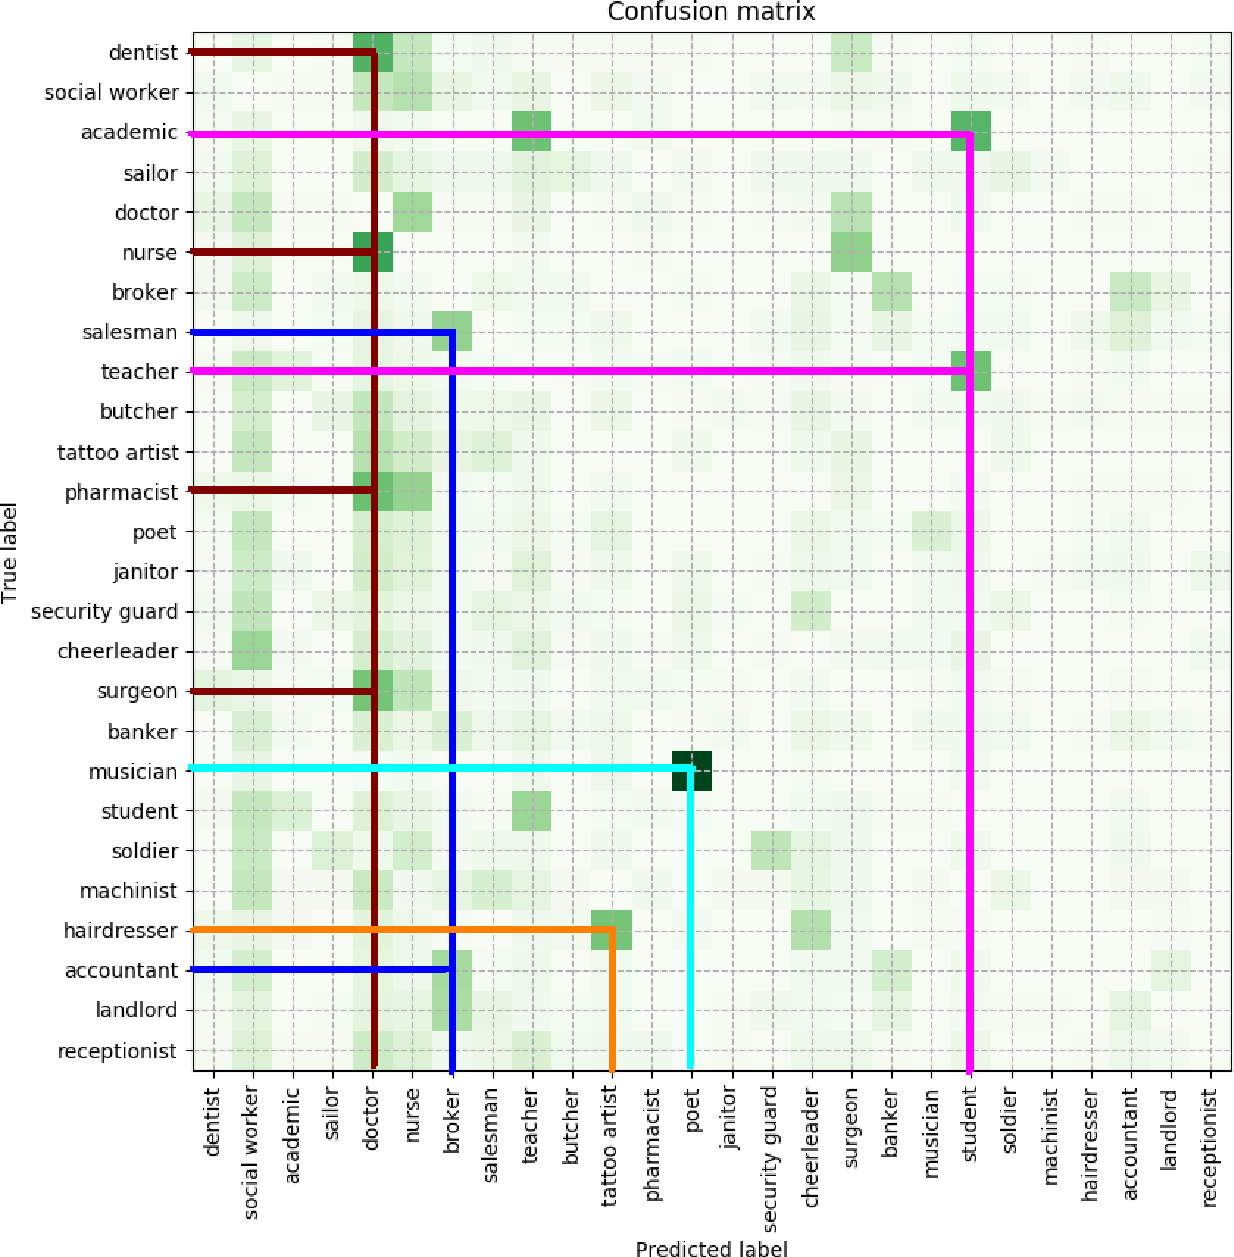
\includegraphics[scale=0.5]{imgs/profession_confusion.pdf}
\vspace{0.3cm}
\caption{Confusion matrix for \emph{profession}  with \charm{KNRM} on \emph{unseen} experiments, with some values removed for brevity. Unseen values are aggregated across folds. 
Darker cells indicate more misclassifications. The lines illustrate misclassifications of interest.
}
   \label{conf_prof}
\end{figure}

%\begin{figure*}[h!]
% \centering
% \begin{subfigure}{.49\textwidth}
%   \centering
%   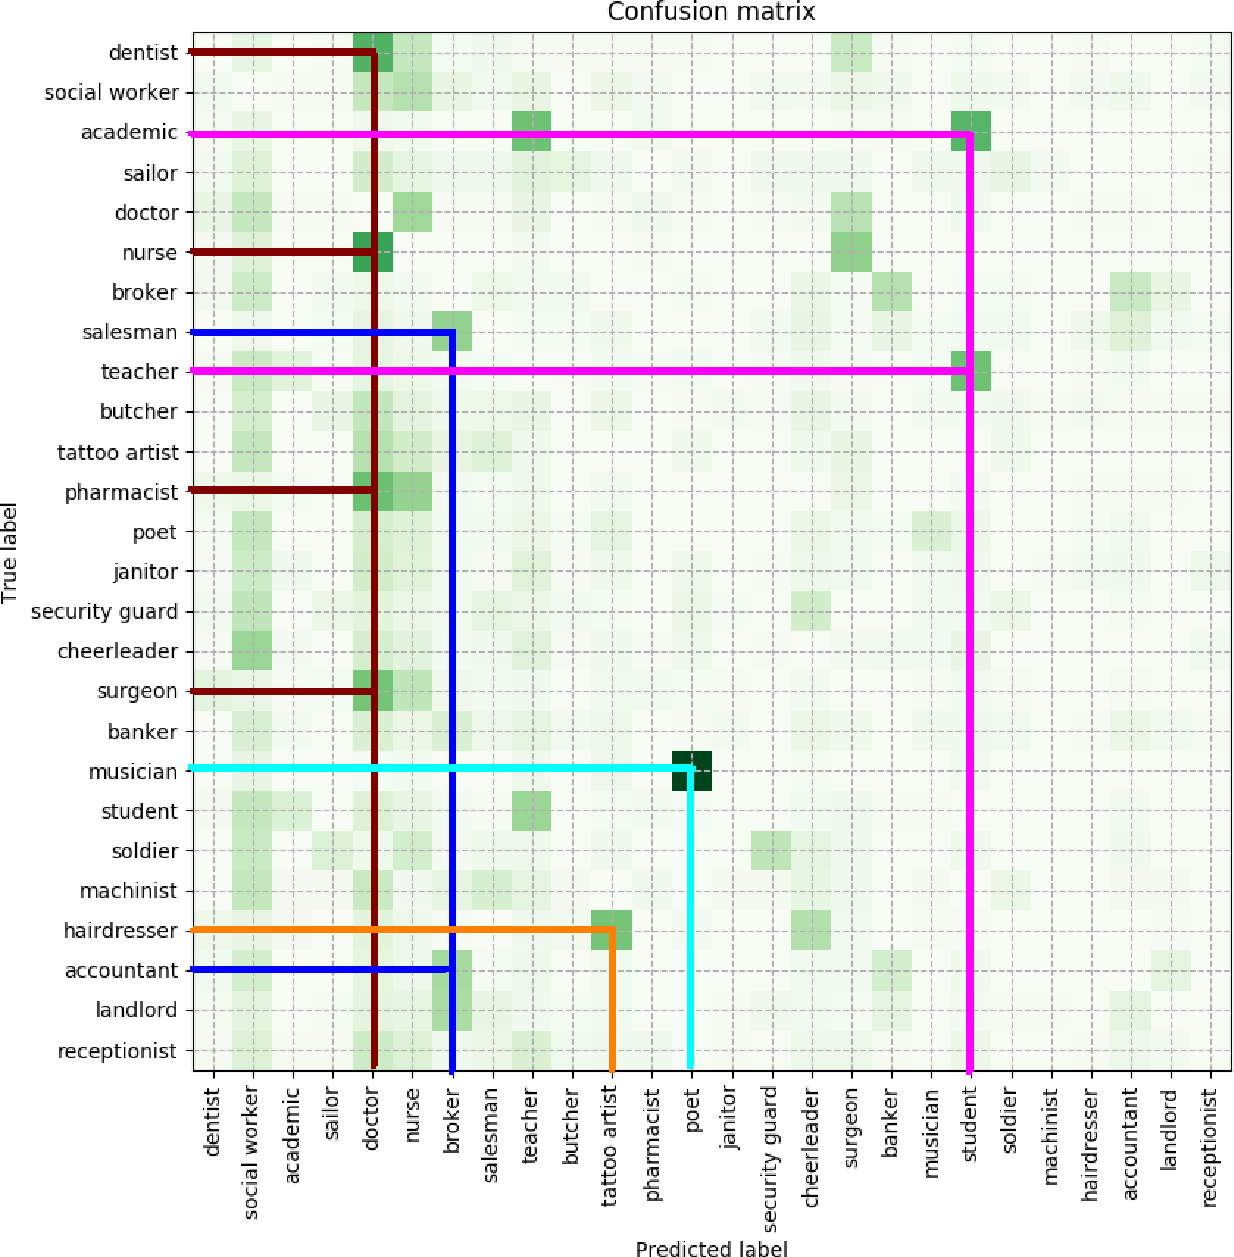
\includegraphics[scale=0.32]{imgs/profession_confusion.pdf}
%   \caption{\textit{profession}}
%   \label{conf_prof}
% \end{subfigure}
% \begin{subfigure}{.49\textwidth}
%   \centering
%   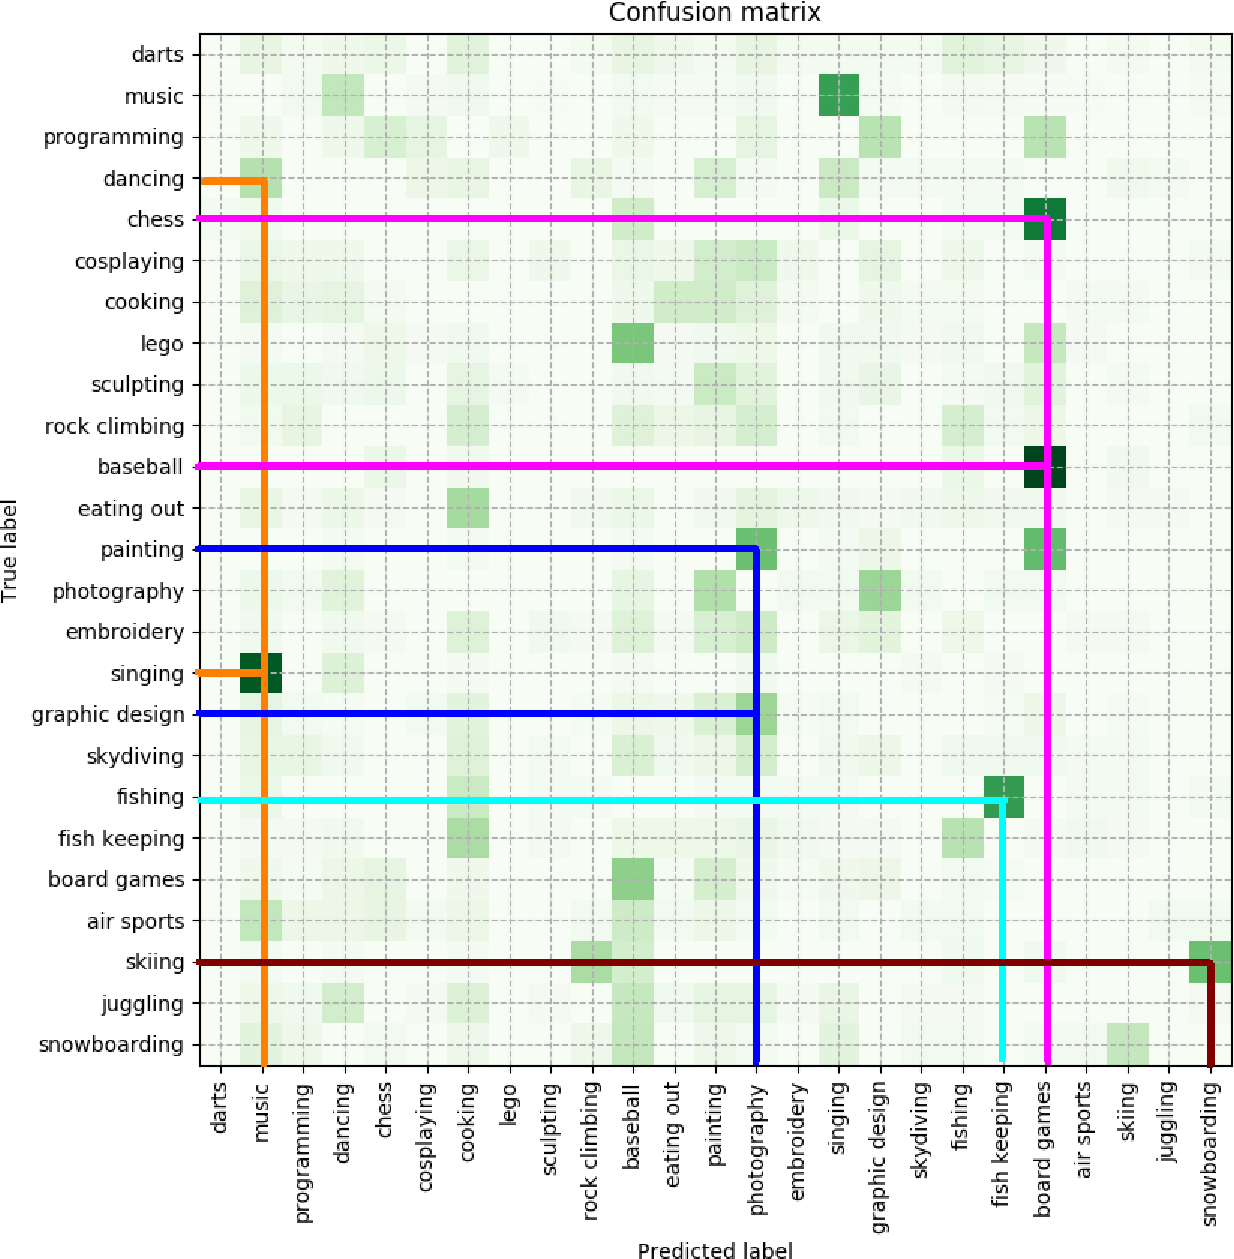
\includegraphics[scale=0.32]{imgs/hobby_confusion.pdf}
%   \caption{\textit{hobby}}
%   \label{conf_hob}
% \end{subfigure}
%\vspace*{-0.3cm}
%\caption{Confusion matrix for \emph{profession} and \emph{hobby} with \charm{KNRM} on \emph{unseen} experiments, with some values removed for brevity. Unseen values are aggregated across folds. 
%Darker cells indicate more misclassifications. The lines illustrate misclassifications of interest.
%}
%\label{fig:conf-profession-hobby}
%\end{figure*}


\paragraphHd{Analysis of top ranked documents}
For each attribute value, we collected all documents that were returned for a user with the given value as the ground-truth label. We then averaged the scores for each document and selected the top 5 retrieved documents from \wiki{category},
shown in Table \ref{tab:top_pages} for several \emph{profession} and \emph{hobby} attribute values.

It is interesting to observe that in spite of the common lexicon for some similar values, the model manages to retrieve documents which are relevant to a particular value, e.g., documents for \textit{investor}  are distinct from other financial-related professions, like \textit{broker} or \textit{salesman}.
It is also worth mentioning that the retrieved pages for \textit{investor} and \textit{ice hockey} are rather the pages for related lexicon (e.g., `\textit{venture capital}' and `\textit{playoff beard}' respectively), which shows the ability of CHARM to detect indirect cues.


\begin{table*}[t!] \sffamily
    \centering
    \footnotesize
    \begin{adjustbox}{width=0.98\textwidth}
    \begin{tabular}{llll}
\toprule
                            \multicolumn{2}{c}{\attribute{profession}} & \multicolumn{2}{c}{\attribute{hobby}}                                                                                                                 \\
\cmidrule(lr){1-2} \cmidrule(lr){3-4}
                            \textbf{firefighter} (MRR=0.46)                & \textbf{investor} (MRR=0.52)                      & \textbf{knitting} (MRR=0.68)                                                & \textbf{ice hockey} (MRR=0.68)                         \\ \midrule
                            Firefighter                                          & Index\_fund                                       & Yarn\_over                                               & Extra\_attacker                                     \\
                            Firefighter\_assist\_and\_search\_team              & Venture\_capital                                  & Brioche\_knitting                                        & Ice\_hockey\_rules                                  \\
                            Calvert\_County\_Fire-Rescue-EMS                    & Treasury\_management                              & Combined\_knitting                                       & Neutral\_zone\_trap                                 \\
                            Firefighter\_arson                                  & Buy\_side                                         & Flat\_knitting                                          & Playoff\_beard                                      \\
                            Fire\_captain                                       & Sovereign\_wealth\_fund                           & Tunisian\_crochet                                        & Line\_(ice\_hockey)                                 \\  \bottomrule
\end{tabular}
    \end{adjustbox}
    \caption{\charm{KNRM}'s top 5 retrieved documents per attribute value.}
    \label{tab:top_pages}
\end{table*}
\section{CHARM Demo}

In this section we present a web demonstration platform, accessible at \url{https://d5demos.mpi-inf.mpg.de/charm}, that showcases CHARM as a predictive model for extracting personal knowledge from conversational utterances \cite{tigunova2021exploring}. The contribution of such system is twofold. First, the demonstration can help users protect their privacy by identifying parts of their generated content that could give away personal information. Second, the system shows in detail how the model arrives at the prediction, which is rarely 
reflected in most automated extraction systems for personal facts.

\subsection{Motivation} 

Personal knowledge is a versatile resource that is valuable for a wide range of downstream applications. As observed in Chapter \ref{chap_backgr}, there has been ample research on automatically extracting or inferring personal knowledge. The developed models for conversational data predict a wide range of personal attributes from basic demographics and personality features to fine-grained interests and biography facts.

Such models can benefit many practical applications, yet they potentially endanger privacy. Thus, users should be given an opportunity to assess how the extraction models work in a transparent way. First, this enables users to explore how much personal information can be revealed from what they say online. Second, this helps to explain the reasoning leading to specific personalized ads and recommendations.

To address this issue we develop a demonstration platform for personal knowledge extraction methods, with CHARM as the underlying model. Such setting gives users a chance to directly observe the model's predictions (as opposed to, for example, trying to interpret the recommendations and ads on the websites).

We demonstrate CHARM's predictive capacity in two possible scenarios. The first setting demonstrates how a chatbot can interact with users to collect personal facts, designed as a guessing game. 
This provides the users with an opportunity to give creative answers and explore the model's capabilities, particularly in inferring the attribute values from given \emph{cues} (e.g., `\textit{pool}', `\textit{paddles}') instead of explicit \emph{mentions} (e.g., `\textit{swimming}'). 
Users can also try out some rare values (e.g., \emph{quilting}) or test how fine-grained the predictions can be (e.g., \emph{curling} instead of \emph{sports}). 
The second scenario involves applying CHARM on the real users' posts on social media. 

The proposed CHARM demonstration enables the users to \emph{(i)} see what personal information is disclosed by their answers or social media posts, and \emph{(ii)} get explanations on how the prediction was made. This supports users' privacy and model's transparency, which are rarely considered by personalized downstream applications, such as search or recommendation engines.

%The top scoring attribute values are yielded by the model as predictions.
%Explanations are given in the form of textual cues found in the input utterances, as well as retrieved web documents used to indicate the attribute values. The users can then identify revealing utterances and see how the predictions change if they modify the lexicon they use. 
%Moreover, we provide an \emph{unseen} mode  to examine how robust the model is for the values that were not seen during training.

\subsection{Demonstration platform}

\label{sec:demo}

Our demonstration system supports prediction of two personal attributes: \textit{profession} and \textit{hobby}, and incorporates two input scenarios: \emph{chatbot} and \emph{social media} settings.

\subsubsection{Input scenarios}

\paragraph{Chatbot setting.} Personal assistants enhanced with background knowledge about their users can give better responses and initiate more interesting conversations.
In this setting, we imitate how an intelligent assistant can infer personal facts from interactions with its user without asking explicit questions, such as \emph{``What is your job?''}. 
The interaction is designed as a game, where the chatbot asks several attribute-related questions, as shown in Figure~\ref{conv}.

\begin{figure}[th!]
\centering
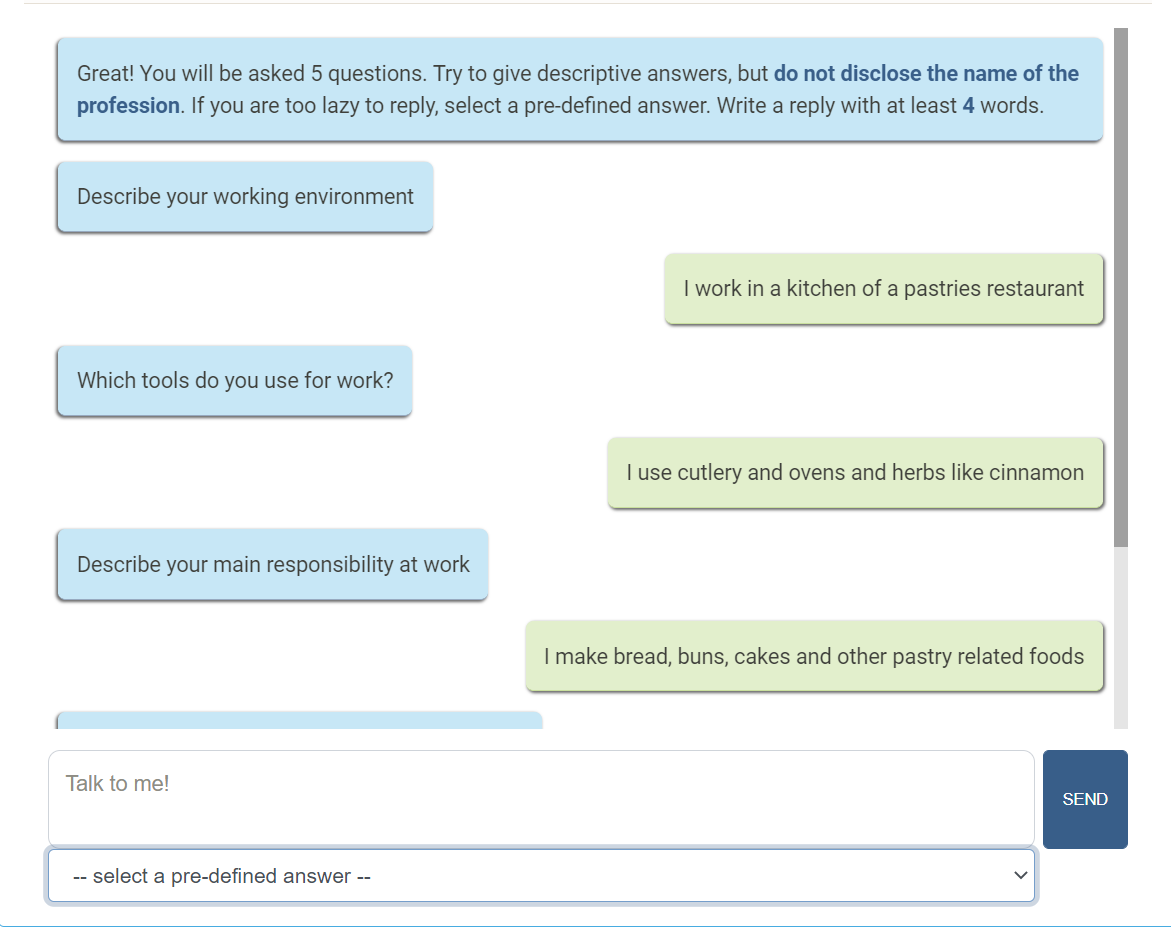
\includegraphics[width=0.85\textwidth]{imgs/conv-baker.png}
\vspace*{-0.3cm}
\caption{Chatbot conversation.}
\label{conv}
\end{figure}

Users are supposed to avoid mentioning the attribute value they have in mind, but rather to provide the chatbot with indirect cues like \emph{``I work in a \textbf{kitchen}''} for the \emph{``Describe your working environment''} question. The number of questions is fixed to 5, which should provide enough cues in the user's utterances to predict the correct attribute value without a lengthy interaction. We also require that the user's response to a question contains at least four words. 

To give users an idea of how responses should look, we provide a sample reply to each question, which the user can choose instead of typing their own responses. Each reply is designed as if it was given by a person with some pre-defined attribute value. For example, for the chat-bot request \textit{``Describe the place where you do your hobby''}, we add a predefined reply \textit{``It is a pool or open water''} related to \textit{hobby:swimming}. 

\paragraph{Social media setting.} 
Social media traces of online users are utilized by large companies for personalizing their services and ads, making them more interesting and relevant. However, the users have neither control nor understanding of how their personal information was inferred and which parts of their content revealed it. Ideally, the users should be given an opportunity to identify and exclude their posts which can potentially expose personal facts. 

In the social media scenario, we show how CHARM 
can dig through the vast amount of 
noisy 
conversational data in social media to find accurate cues for prediction.
Users can type or paste their social media posts (e.g., Reddit submissions) into the social media interface of our demonstration platform. Together with CHARM's predictions, the users will be provided with the information which parts of their utterances were used by the predictive model. It provides an opportunity to delete or modify the exposing content, and to check whether the model can still arrive at the same prediction after a partial content removal.

As in the chatbot scenario, we provide samples of synthetic user-generated content, resembling submissions in Reddit discussion threads, corresponding to pre-defined attribute values.
%that are often noisy, colloquial and unstructured.


\begin{figure}[th!]
    \centering
    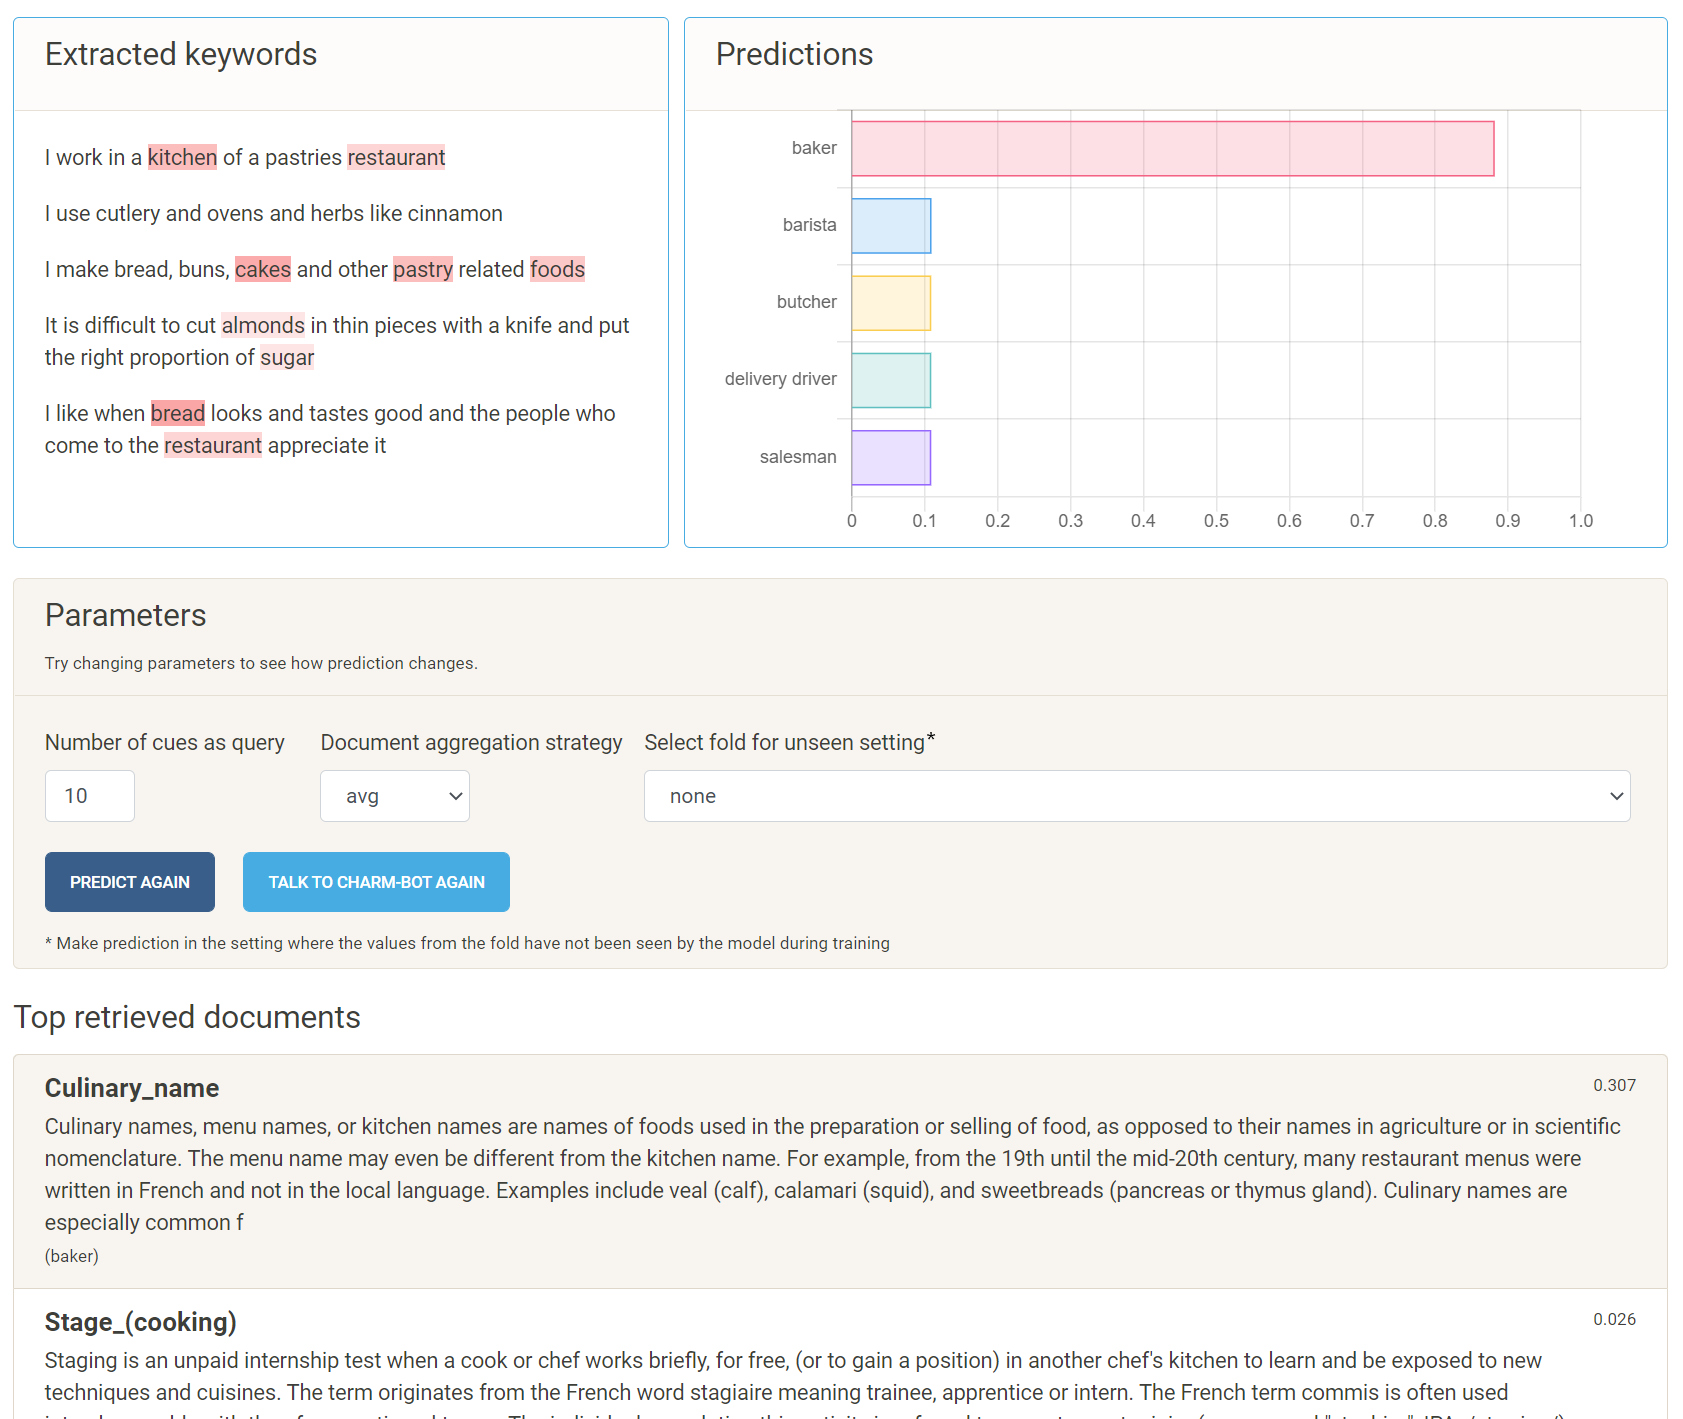
\includegraphics[width=0.95\textwidth]{imgs/prediction-baker.png}
    \caption{CHARM prediction result.}
    \label{pred_img}
\end{figure}

\subsubsection{Prediction results} 
As shown in Figure \ref{pred_img}, the prediction page presented to the user consists of intermediate results for both components of CHARM (\textit{term scoring model} and \textit{document ranker}) and the final prediction. To show the keyword selection step, we highlight the words in the user's utterances with an intensity that corresponds to the words' scores given by the {term scoring model}. The results for the document ranking step are presented as a sorted list of 10 top scoring documents. Each document is linked to the original article on the web. Finally, we show top 5 attribute value predictions after aggregating document scores. We normalized them to $[0,1]$ scale for interpretability when comparing the model's confidence in predicting each value. 

\subsubsection{Model parameters} 
The demonstration allows the users to explore how CHARM's predictions change depending on its two hyperparameters: the \emph{number of extracted keywords} and the \emph{document aggregation strategy}. 
We set the default number of extracted keywords as $\frac{1}{3}$ of the number of meaningful terms in the input utterances (after removing stopwords and digits), 
with 10 as the maximum value.
Setting the number of keywords too high can result in a noisy query and inadequate behaviour of the retrieval model. 
On the other hand, small number of keywords can be insufficient for accurate document retrieval.

As the document aggregation strategy, the user can choose between \texttt{max} and \texttt{average} functions. \texttt{Max} operation is useful when the document collection is noisy and the prediction score should come from a single most relevant document per attribute value. The \texttt{average} function is good to provide a balanced prediction based on all available documents, protecting the result from being spoilt by an inappropriate top scoring document. For this reason we selected \texttt{average} as the default aggregation function.

We selected to use \charm{KNRM} as the underlying model and \wiki{category} as document collection for our demonstration platform. As shown in the experiments described in Section \ref{charm_results}, this combination of ranker and document collection shows superior performance in most test cases. \wiki{category} is a sweet spot between simple \wiki{page}, which can only provide trivial explanations with pages matching attribute value name, and Web-search collection, which is difficult for the end-user to interpret because of noisy and ill-formatted pages. %On the other hand, \wiki{category} shows how CHARM's predictions can be determined by the topical pages from the same category.
 
\subsubsection{Unseen scenario} 
We also showcase CHARM's ability to predict attribute values
that are lacking training samples.
We train 10 variants of the model, in which each model has seen samples from only 90\% of the attribute values during training; 10\% of the attribute values are \emph{unseen}. 
In our web interface, the users can try to make a prediction using one of those models
by selecting the option where the listed attribute values are unseen. 
For example, for the input utterances \{\emph{``I was pedaling the whole evening''}, \emph{``I don't like long walks, I like spending time on my bike''}\}, it can be interesting to see the prediction result by the model not trained on hobby value \emph{cycling}. 

\subsection{Case study}
\label{sec:case-study}

In this section we present a walk-though scenario for the chatbot setting. As input we take a set of utterances from a pre-defined personality having \textit{profession}: \textit{baker}. In the first step, the chatbot asks the user 5 questions, such as \emph{``How do you start your day at work?''}. We give an excerpt of the conversation between the user and the chatbot in Figure \ref{conv}. 

On the next step the user is taken to the prediction result page, shown in Figure~\ref{pred_img}. Using the default heuristic, CHARM extracts \nolinebreak 9 keywords from the input.
The resulting query thus becomes \textit{``kitchen restaurant cakes pastry foods almonds sugar bread restaurant''}. From Figure \ref{pred_img} it can be seen that the words `\textit{cakes}', `\textit{bread}' and `\textit{pastry}' were assigned high scores by the term scoring model, whereas more general words, like `\textit{restaurant}', were included in the query but received lower scores.

The default document score aggregation strategy is \texttt{average}, which helps to overcome the influence of the top scoring document \emph{wiki:Stage\_(cooking)} (a culinary internship), which was automatically labeled as \textit{student}. 
Thus, if the user changes the aggregation function to \texttt{max}, the effect of document scoring makes \emph{baker} and \emph{student} almost equally probable. 

The qualitative results of varying the parameters of CHARM on our exemplary input are shown in Table \ref{param_change}. 
Setting the number of keywords to 2 still does not prevent CHARM from making a correct prediction using a concise query \textit{``bread ovens''}. However, the model is not robust with a long query, resulting in the ranker yielding many documents equally relevant to this query, like \emph{baker}, \emph{barista} and \emph{butcher} pages.

Finally, the user can inspect the behaviour of CHARM in the \emph{unseen} setup, when the value \emph{baker} was not present in the training data. To do that the user should select an unseen fold from the dropdown list, which contains the value \emph{baker}. As shown in Table \nolinebreak\ref{param_change}, CHARM is still capable of predicting the correct value. In contrast to the normal \textit{seen} setting, the difference in scores for correct and incorrect predictions is less.

\begin{table}[]
    \centering
\begin{adjustbox}{width=0.75\textwidth}
\begin{tabular}{ccc|cl}
\toprule
\begin{tabular}[c]{@{}c@{}}number of \\ keywords\end{tabular} & \begin{tabular}[c]{@{}c@{}}aggregation \\ strategy\end{tabular} & \begin{tabular}[c]{@{}c@{}}seen/unseen \\ setting\end{tabular} & \begin{tabular}[c]{@{}c@{}}correct \\ prediction score\end{tabular} & \begin{tabular}[c]{@{}c@{}}best incorrect \\ prediction score\end{tabular} \\ \midrule
10                                                            & avg                                                             & seen                                                           & 0.91                                                                & 0.19 (barista)                                                                      \\
\textbf{2}                                                    & avg                                                             & seen                                                           & 0.88                                                                & 0.19 (sailor)                                                                      \\
\textbf{25}                                                   & avg                                                             & seen                                                           & 0.85                                                                  & 0.85 (barista)                                                                      \\
10                                                            & \textbf{max}                                                    & seen                                                           & 0.89                                                                & 0.77 (student)                                                                       \\
10                                                            & avg                                                             & \textbf{unseen}                                                & 0.91                                                                & 0.32 (butcher) \\                      \bottomrule                                  
\end{tabular}
\end{adjustbox}
    \caption{Prediction scores based on CHARM parameters.}
    \label{param_change}
\end{table}
\section{Conclusion}
We presented the 
Conversational 
Hidden 
Attribute 
Retrieval 
Model (CHARM), a novel method 
for inferring personal traits from conversations. CHARM differs from prior
work by its zero-shot ability to
predict attribute values 
that are not present in the training samples
at all.

We demonstrated 
the viability of CHARM
for inferring users' unseen attribute values
by comprehensive 
experiments with Reddit conversations on \textit{profession} and \textit{hobby} attributes,
leveraging document collections from Wikipedia and web search results
for CHARM's retrieval component.
In the zero-shot setting CHARM shows significantly better performance than existing unsupervised keyword selectors, especially given the challenging conversation domain. Moreover, CHARM also performs on par with state-of-the-art fully supervised models in the regular classification setting.

CHARM is extensible to other long-tailed personal attributes, such as \textit{favorite food type} or \textit{preferred travel destination}, without changing the model's architecture or exhaustive manual effort to construct external document collections. Moreover, the components of CHARM, \textit{term scoring model} and \textit{retrieval model} are easily modifiable, allowing to plug in any emerging state-of-the-art architecture. Finally, the strength of CHARM is its end-to-end training, without any intermediate supervision steps, regardless of the absence of ground truth about the attribute values' keywords.

We have shown that CHARM's predictions are explainable by the keywords and documents it selects, which are sufficiently descriptive to enable CHARM to draw fine-grained distinction between similar attribute values. To showcase that, we created a web demonstration platform, enabling the users to interact with CHARM and explore its predictions. Such web service will be a helpful asset to provide the end users with transparent and explainable models. 

As future work directions we see improving CHARM's performance in the seen setup and applying the model on further datasets, given the availability of the labeled samples. Moreover, as CHARM's ability to make predictions in the unseen setup heavily hinges on the external document collection, it is interesting to explore different sources and methods to collect the documents. As we have observed, both comprehensive and diverse collections (automatically created web search collection) as well as highly precise collections with little noise (manually refined \wiki{category}) can strengthen the performance on different attributes.

We envision a major extension of CHARM as the model, capable of predicting \textit{open-ended} personal attributes, such as \textit{favorite singer}. For such attributes it is impossible to create comprehensive lists of attribute values, especially given constantly emerging new entities. This problem can be tackled by means of zero-shot learning techniques with heavy reliance on external information sources, such as knowledge bases.

\chapter{Predicting Relationships in Dialogue Excerpts}
\label{chap_pride}
\minitoc
%Interpersonal relationships greatly influence how we talk, shaping speech style and the choice of words in daily conversations. 

\droppedcapital{A}{utomatically}
extracted
interpersonal relationships of conversation interlocutors
can enrich
personal knowledge bases  
to enhance personalized search, recommenders and chatbots.
In this chapter we propose PRIDE: a
neural multi-label classifier inferring speakers' relationships from dialogues.
Compared to the general models for structured texts,
PRIDE can effectively utilize the dialogue structure additionally augmenting it with external knowledge about 
speaker features and conversation style.
Unlike 
prior works,
we 
address 
multi-label prediction of fine-grained directed relationships. Extensive experiments on datasets based on screenplays of movies and TV series show superior performance of PRIDE compared to the state-of-the-art baselines.
\section{Introduction}

\noindent{\bf Motivation and Problem.} A Personal knowledge base enhanced with the information about the users' interpersonal relationships is practical for many applications. For example, relationship facts in a PKB can be accessed by a personalized chat-bot, which will enable it to make better suggestions for the user (for example, suggesting that the user takes her \textit{child} to the zoo instead of a romantic dinner). Moreover, the speech style of the chat-bot, varying from neutral and official to casual and friendly, can be adjusted based on the relationship between the user and her current interlocutor. Finally, if the conversation happens over the phone, the underlying software can automatically assign categories (family/business/..) for the contact list of the user's interlocutors.

With the ubiquity of social media and online forums, user-generated content is available in abundance. Mining personal knowledge from user-generated content to populate PKBs, or \emph{user profiling}, is a long-standing topic in NLP \cite[e.g.,][]{flekova:ACL16:long,basile:2017,tigunova2019listening}. While users' demographic attributes and interests can be learned from their profile descriptions and posts, interpersonal relationships with other users are rarely mentioned explicitly and may only be inferred from their interactions and conversations.

In this work, we develop an automatic method for predicting fine-grained relationships between two speakers, given their logged conversation history.

\begin{figure}[t!]
\centering
\begin{adjustbox}{width=0.46\textwidth}
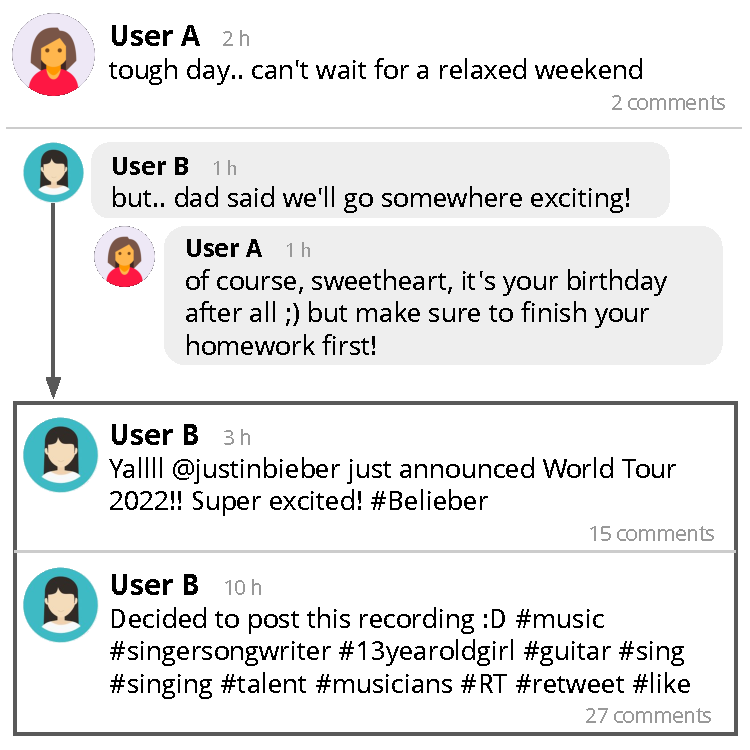
\includegraphics{imgs/conversation_example}
\end{adjustbox}
\caption{Example of 
conversation in social media.}
\label{example_conv}
\end{figure}

Consider the example in Figure~\ref{example_conv}.
From the excerpt of interactions between A and B, the reader can figure out that B is the \textit{child} of A by observing \textit{(i)} the address term `sweetheart', \textit{(ii)} the commanding but soft tone of user A, \textit{(iii)} the reference to the other family member `\textit{dad}', and \textit{(iv)} the context created by the word `\textit{homework}'. Yet, neither of the speakers directly mentions their relationship, making this task difficult for automatic methods 
relying on explicit pattern matching or keyword search.

The relationship information extracted from such conversations, e.g., \textit{<B, child\_of, A>}, can be entered into the PKBs of users A and B. By combining such relationship information with User B's age and personal interests (e.g., \emph{playing guitar, Justin Bieber}) inferable from User B's social media (exemplified in Figure~\ref{example_conv}), 
a system will be able to provide
user A with relevant personalized recommendations for a query ``\textit{birthday present ideas for my daughter}''. 

\paragraphHd{Prior Work and its Limitations.} There has been considerable research on extracting relationships between characters in literary texts such as novels \cite{chaturvedi2016modeling, chaturvedi2017unsupervised}. These methods are inappropriate for conversational data, though, 
which is colloquial and less structured than literary texts. 
Moreover, 
predicting relationships is often  modeled as a binary task of sentiment classification (i.e., person A is positive or negative about person B). 
Prior works on conversational data
are restricted to
small-scale data \cite{yu-etal-2020-dialogue}, or merely handle coarse labels of relationship aspects \cite{rashid2018characterizing,qamar2021relationship}. Most approaches use general models for text classification \cite{chen2020mpdd,jia2020ddrel}, which 
disregard the particularities of
conversational settings. 

\paragraphHd{Approach and Contributions.} We present PRIDE, a 
neural multi-label classifier for \textbf{P}redicting \textbf{R}elationships \textbf{I}n \textbf{D}ialogu\textbf{E}. 
PRIDE makes inference among 12 fine-grained directed relationships (like \emph{child} or \emph{boss}) from conversational data by hierarchically creating utterance representations and combining them with signals on the users' personal attributes (e.g., \textit{age} and \textit{occupation}) and the conversation style (e.g., \textit{intense} or \textit{superficial}).
PRIDE uses BERT \cite{devlin2019bert} to create contextual word embeddings for each utterance, and Transformer encoders \cite{vaswani2017attention} to build conversation representations that preserve information about the sequence and speakers of utterances.

The contributions of this work are: 
\squishlist
\item a method for inferring speakers' relationships from conversational data, which outperforms strong baselines; 
\item an exhaustive analysis of the model's performance. We perform various experiments assessing PRIDE's transfer-learning capabilities and robustness to the varying lengths of the input conversations. Additionally, we conduct ablation studies, proving that all components of the model are essential for the accurate prediction of interpersonal relationships.
\squishend
\section{Related Work}

The models HAMs and CHARM, described in the previous two chapters, make predictions based on the input from a single speaker. Meanwhile, relationship inference requires processing the utterances of a pair of interlocutors in a conversation.
In this section we will summarize related work on modeling multi-speaker dialogues. Many natural language processing tasks based on conversational speech (chatbot answer generation, utterance intent classification, emotion prediction, etc.) require creating a representation of a given multi-speaker conversation as input.
We identify several features typical of the conversational data, which can be used to enhance predictive models: \textit{(i)} conversational structure, \textit{(ii)} speaker attribution, \textit{(iii)} additional speaker information. 

\paragraph{Conversational structure.} 
One popular way to represent a conversation is to model words and utterances in a hierarchical manner. Hierarchical approaches are widely applied to microblog sentiment and emotion classification. We gave a comprehensive overview of the hierarchical models in Section \ref{ham_hier}; in the current section we recap several recent methods, which inspired the choice of our model's architecture.

The core idea of hierarchical modeling is to create the representations of words, which are aggregated to create the representations for utterances; the latter are either used in the utterance-level inference or are further combined to make predictions on the conversational level. 

A number of related studies use BERT to create the contextual representations of words, which are then processed by the recurrent models to form the representations of utterances \cite{lei2019bert, ma2020han}. This approach is still not optimal because RNNs can not effectively capture the dependencies in the long input sequences and suffer from vanishing gradient. An alternative approach is to create utterance representations with Transformer \cite{shan2020contextual, li2020hierarchical}; our proposed architecture also follows this approach. In contrast to prior works, the distinguishing feature of our method is an effective way to overcome the limitation on the number of BERT input tokens. As opposed to cropping or processing single utterances out of context \cite{li2020hierarchical, shan2020contextual}, we process the whole input conversations in large chuncks, joining them into a unified context with Transformer.

Another way to utilize dialogue structure is to use a graph to represent the conversation. Such approaches are used to process multi-party conversations involving more than 2 speakers, which often have non-sequential structure, as a single utterance can have multiple responses to it. An intuitive way to model such conversations is to use utterances as the vertices in a dialogue graph; an edge will then connect the response to its parent utterance~\cite{hu2019gsn}. Alternatively one can exploit a fully-connected graph \cite{ghosal2019dialoguegcn}, under the assumption that all utterances influence each other. Graph-based modelling has proven to be effective on natural language tasks such as emotion classification \cite{zhang2019modeling, ghosal2019dialoguegcn}. However it is unnecessary for out setting, as we consider only dyadic dialogues, modeling utterances' interactions with Transformer. %Moreover, a complete graph can always be modeled with a Transformer, which we use in our method.

\paragraph{Speaker attribution.} Speaker attribution (the information which speaker the current utterance was produced by) is often used across various NLP tasks to create speakers' representations. For example, in utterance addressee identification \cite{le2019speaking, ouchi2016addressee} the models are trained to produce speakers' embeddings, which are explicitly used for addressee prediction. In other NLP tasks, such as sentiment classification or response selection, the learned speaker representations are blended into the model to enhance its performance.

To equip Transformer with speaker information, the studies by \citet{liu2021filling} and \citet{li2020hierarchical2} leverage specialized input masks to distinguish utterances from different speakers. These masks create distinct channels for each speaker in the encoder, so that an utterance representation can attend to the input from each speaker separately.

A simple but effective way to blend in speaker information into Transformer-based models, such as BERT, is to introduce additive speaker embeddings on the word level. For dyadic conversations, speakers are usually distinguished using BERT's segment embeddings~\cite{lu2020improving}; for the conversations with more than two speakers a common solution is to 
add a separate speaker embedding layer into BERT's embedding module \cite{gu2020speaker, yu-etal-2020-dialogue}.

PRIDE also incorporates speaker information; we add learned speaker embeddings to the Transformer input on the utterance level, following \citet{li2020hierarchical}, as well as using BERT's segment embeddings as speaker indicators on the word level.

\paragraph{Additional speaker information.} Knowing the speaker of each utterance enables to link the available external knowledge about that speaker, making the model's predictions more accurate. There has been significant research on creating response selection models infused with pre-defined speaker personality \cite{mazare2018training, zhang2018personalizing}. Such approaches operate on the utterance level, attaching personality to each generated utterance. As opposed to it, \citet{welch2019look} enriched the model for speaker attribute prediction on the global (conversation) level, adding various features of the interlocutor, such as relative age or gender. Inspired by this approach, we also enhance our model with the information about the speakers' ages.





\section{Background}
\label{background}

Interactions between people can have multiple fine-grained features, describing various aspects of their communication. For example, interactions can be characterized by attachment style (such as \textit{commitment} or \textit{avoidance}) \cite{qamar2021relationship} or power hierarchy (\textit{subordinate} or \textit{superior}) \cite{prabhakaran2014predicting}. There are ample related social studies researching these characteristics; yet, there is no formal ontology for them \cite{rashid2018characterizing}. One way to organize the features of interpersonal interactions was proposed by \cite{rashid2017dimensions}, defined as \textit{dimensions} of the relationships.

Most of the relationships that we defined for our experiments also have particular interpersonal characteristics. For example, the \textit{enemy} relationship can be described as \textit{competitive} as opposed to \textit{cooperative}; the relationship between \textit{parent} and \textit{child} is in most cases \textit{intimate}. Thus, we find it beneficial to enhance the relationship prediction model with the known features of the speakers' interactions. 

We use the definition of \textit{interpersonal dimensions} \cite{wish1976perceived} of speakers' interactions and relationships, following classification of \citet{rashid2018characterizing}, which we used as an additional input to our model. We note that the discussed interpersonal dimensions are descriptive of the relationship between a particular pair of speakers, but not of the relationship type in general (for example, the interaction between \textit{colleagues} can be both \textit{cooperative} and \textit{competitive}). However, in general any interpersonal dimension can be more or less typical for a relationship type; we use this information to give the model hints about applicable predictions.

\citet{rashid2018characterizing} consider 11 interpersonal dimensions, divided into dimensions of relationships and interactions, as shown in Table \ref{dimensions}. In our model we use all proposed dimensions to provide a comprehensive summary of the relationship's fine-grain characteristics. %For details on each dimension we refer the reader to the original paper \cite{rashid2018characterizing}.
\citet{rashid2018characterizing} also provide a conversational dataset, where every utterance has annotations for each considered interpersonal dimension. We utilize this dataset to pretrain a model for utterance-level dimension classification and create separate representations for each dimension, which are later used in PRIDE.

\begin{table}[t!]
\centering
\begin{adjustbox}{width=0.7\textwidth}
\begin{tabular}{@{}l|ll@{}}
\multirow{4}{*}{relationships} & cooperative vs. noncooperative & equal vs. hierarchical\\ 
 & pleasure vs. work oriented & intense vs. superficial \\ 
 & intimate vs.unintimate & active vs. passive \\ 
 & temporary vs. long term \\ \hline
\multirow{2}{*}{interactions}  & cooperative vs. noncooperative & active vs. passive \\ 
 & concurrent vs. non concurrent & near vs. distant \\                                                          
\end{tabular}
\end{adjustbox}
\caption{Interpersonal dimensions used in PRIDE.}
\label{dimensions}
\end{table}



\section{Methodology}

The design of our model is based on conversational features such as dialog structure (the order and boundaries of the utterances) and the attribution of each utterance to its corresponding speaker. The model architecture, inspired by \citet{li2020hierarchical}, is shown in Figure \ref{pipeline}. PRIDE hierarchically creates word and utterance representations, which are then combined with representations of personal attributes and interpersonal dimensions (Table \ref{dimensions}) to create a representation of the full conversation history.
Given this representation of the conversation, a multi-label classification layer predicts one or more of the relationship labels, listed in Table \ref{perclass}.
The model is trained with supervision on the relationship labels.
In the following subsections we describe the model's components in more detail.

\begin{figure}[t!]
\centering
\begin{adjustbox}{width=0.6\textwidth}
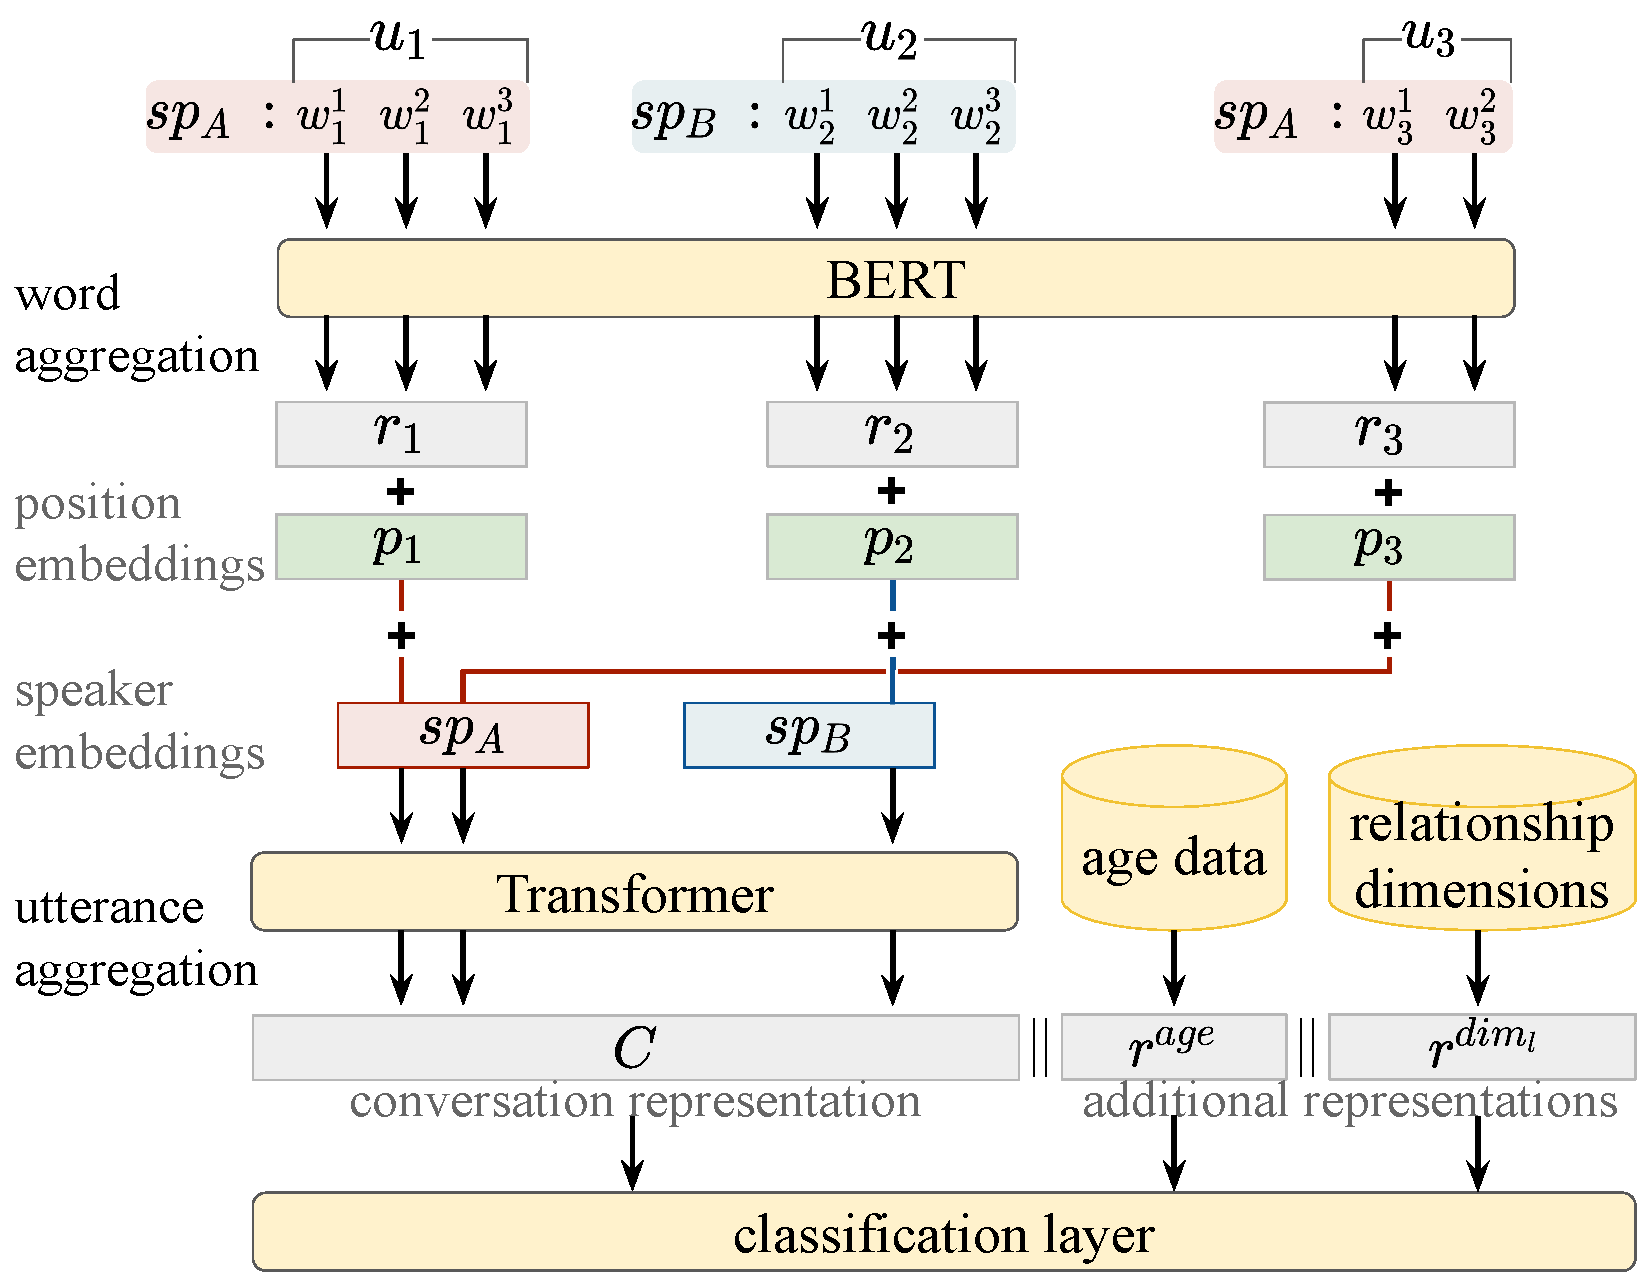
\includegraphics{imgs/PRIDE_scheme_3}
\end{adjustbox}
\caption{PRIDE model}
\label{pipeline}
\end{figure}

\subsection{Contextual word representations}

The input for a pair of speakers ($sp_A$, $sp_B$) is $N$ utterances $u_1, ... u_N$, where $i$-th utterance consists of words $w_i^1, ... w_i^{n_i}$. 
In the first step, the word representations $r_i^j$ are created with a function $f^{word}(w_1^1,..,w_1^{n_1},...,w_N^{n_N})=r_i^j$, which takes as input the concatenation of all utterances and produces the representations for each word. We chose BERT \cite{devlin2019bert} to create word representations, because this model efficiently captures contextual information.

Considering that the maximal input length of BERT is 512 tokens, we split the input sequence of utterances into chunks and run BERT several times. Each chunk in the split has the maximal possible length that fits into one run without breaking individual utterances. We find this splitting strategy more effective than running BERT on single utterances~\cite{chen2020mpdd} or short sequences which don't fully utilize max 512 limit \cite{jia2020ddrel}. In our method more conversational context is provided to create word representations. Also, simply truncating input to 512 tokens \cite{lu2020improving} might cause a loss of important cues. 

As information about the current speaker we use BERT's segment embeddings, so that the A-segment corresponds to tokens from $sp_A$ and the B-segment to $sp_B$.
Furthermore, we encode the information about the utterance boundaries by prepending special tokens before each utterance: $[\textrm{s1}]$ for the utterances of speaker A and $[\textrm{s2}]$ for speaker B. 

\subsection{Utterance representations}

Next, word representations $r_i^j$ are aggregated within each utterance to create utterance representations $r_i$ with the aggregation function $a^{word}(r_i^1,...r_i^{n_i})=r_i$. The aggregation is performed on the utterances from all runs of BERT and outputs $r_1, ... r_N$ as the representations of utterances.
In our hyperparameter search we tried instantiating $a^{word}$ with \textit{max}, \textit{average} and \textit{self-attention weighted average} functions.

Some of $r_i$ are been produced by separate runs of BERT due to its input length limitation. Therefore we create enriched utterance representations in the unified context from all BERT runs with the function $f^{utt}(\hat{r}_1,...,\hat{r}_n) = \tilde{r_i}$. We instantiate $f^{utt}$ with a Transformer encoder, which allows us to input long sequences of utterances. 
Before computing enriched representations, we sum the utterance representations $r_i$ with sinusoidal positional encoding $p_i$ and speaker embeddings $sp_i$, yielding $\hat{r_i} = r_i + p_i + sp_i$. The speaker embeddings are randomly initialized and learned during model training. Positional encoding is performed following \citet{vaswani2017attention}. 

\subsection{Classification layer}

\sloppy Finally, the enriched utterance representations $\tilde{r_i}$ are aggregated with the function ${a^{utt}(\tilde{r_1},...\tilde{r_n})=C}$. $a^{utt}$ is instantiated with the same aggregation functions as $a^{word}$. For the case with $[\textrm{CLS}]$ representation we prepend a trainable embedding to the sequence.

We incorporate additional information relevant to the relationship prediction by concatenating embeddings of personal attributes and interpersonal dimensions with the conversation representation $C$: $\tilde{C} = C|r^{age}|r_{dim_l}$, which are described in the following subsections.
A fully connected layer takes the resulting concatenated representation $\tilde{C}$ as input and produces probability scores for each of $L$ relationship labels. Since some relationships are not symmetric (e.g., \emph{parent/child}) the labels represent directed relationships from $sp_A$ to $sp_B$.


\subsection{Incorporating personal attributes}

Additional personal information about the speakers from a personal knowledge base, such as their \textit{age} or \textit{occupation}, could improve relationship prediction.
We incorporate \textit{age} information into the model, since some relationships in our dataset can commonly be characterized by age differences between the speakers. For instance, children are usually much younger than their parents (and a parent can never be younger than a child). Similarly, employees are generally younger than their bosses (but the magnitude of their age difference is less than in parent/child pairs). Among all possible personal attributes we select to incorporate only age difference for two reasons: \textit{(i)} other labeled personal attributes are very scarce and difficult to obtain, and \textit{(ii)} other attributes, such as \textit{gender}, are not nearly as informative as speakers' age difference. Nevertheless, the architecture of PRIDE can easily include any number of additional attributes (e.g., \textit{profession}, \textit{family status}, etc.).

To incorporate age information into PRIDE, we introduce a representation for the age difference of speakers. We calculate $(age_A - age_B)$ and assign the resulting difference into an age difference bin.
We learn an $m$-dimensional embedding $r^{age}$  for each bin, where $m$ is a hyperparameter optimized in the grid search.

\subsection{Incorporating interpersonal dimensions}

As discussed in Section \ref{background}, interpersonal relationships have fine-grained characteristics, called \textit{dimensions} \cite{wish1976perceived}. For instance, a \textit{boss/employee} relationship is hierarchical, while \textit{colleague} is an equal one. Similarly, \textit{spouse} is an intimate relationship, in contrast to \textit{colleague}.

Given a hint of the applicable dimensions, a model can better predict the underlying relationship (e.g., a \textit{non-intimate}, \textit{task oriented} and \textit{hierarchical} relationship is most likely a \textit{boss/employee} relationship). Based on \citet{rashid2018characterizing}, we distinguish 11 interesting interpersonal dimensions, listed in Table \ref{dimensions}. 

Using the data provided by \citeauthor{rashid2018characterizing}, we train a separate BERT classifier on the utterance level for each dimension $dim_l$, where index $l$ ranges over the 11 interpersonal dimensions we used.
We obtain a $K$-dimensional CLS representation from the trained classifier for each utterance, thus producing a $K$-dimensional representations $r^{dim_l}_i$ for the $i$-th input utterance.
To incorporate these representations into our model, we obtain a single representation $dim_l$ at the conversation level by performing max pooling over all utterance representations for a given speaker pair.


\section{Experimental setup}

\subsection{Data splitting and preprocessing.} 
For experiments with PRIDE we used Film Relationship (FiRe) dataset, described in Section 3.1.2.
From the input scripts we removed personal names\footnote{
%Based on the list in 
\href{https://catalog.data.gov/dataset/baby-names-from-social-security-card-applications-national-data}{\texttt{\justify https://catalog.data.gov/dataset/baby-names-from-social-\\security-card-applications-national-data}}} and movie-specific words (which we defined as words found in only one movie script), to reduce overfitting to movie domain or genre.

We performed five-fold cross-validation, training the models on three folds and choosing hyperparameter settings according to the performance on 1-fold validation set. We report the results on the remaining 1-fold test set. We arranged the folds so that the sets of movies, where the input character pairs come from, are disjoint. With that as a hard restriction, we tried to maximally balance the label distributions across the folds. For that we created multiple random assignments of movies to folds and chose the one that maximized the balance metrics, which we defined as follows:
\begin{gather*}
    label\_balance = mean([\frac{d_l}{S_l} \mbox{ for l in labels}]), \\
    d_l = \max_{i}s^i_l - \min_{i}s^i_l, 
\end{gather*}
where $S_l$ denotes the number of pairs for the label l in the whole dataset, and $s^i_l$ denotes the number of pairs for the label $l$ in fold $i$.


\subsection{Model setup and evaluation metrics}

We fine-tuned a pretrained BERT model (bert-base-uncased) to create word embeddings. To produce interpersonal dimension embeddings, we train BERT on the labeled data from \citet{rashid2018characterizing} on each dimension separately, resulting in 768-dimensional representations.

We gathered the data about speakers' ages by crawling \url{imdb.com} for the ages of the corresponding actors in the year the film/series was made. To create age embeddings we calculate the age difference (\emph{diff}) between the speakers and assign it to one of the predefined \emph{diff} bins. We set \emph{diff} bins to be [(-inf; -13], [-12; -6], [-5; -1], [0; 4], [5; 11], [12; +inf]] (a negative age difference means that speaker B is younger than speaker A).

\paragraphHd{Training mechanism.} PRIDE is trained in two steps: first we train the model without external representations (age difference and interpersonal dimensions). The pretrained base model checkpoint is then used in full PRIDE to train external representations' embeddings and classification layer (the weights of the base model stay frozen).

We trained the model with Binary Cross Entropy loss. During training we oversampled the under-represented labels. We perform grid search to tune the following hyperparameters: training epoch, learning rate (we use different learning rates for BERT and the rest of the model), word and utterance aggregation (among \textit{max}, \textit{average} and \textit{attention}).
We perform multi-label classification by predicting all labels with a score over a threshold, which we treat as a hyperparameter.

\paragraphHd{Evaluation metrics.} We compute macro-averaged multilabel precision, recall and F1 score as evaluation metrics. During grid search we optimized F1 score of the performance on the development set.

\subsection{Baselines.}
 We compare the performance of PRIDE with the following baselines:
 \squishlist
     \item \textbf{RNN} is a BiLSTM \cite{graves2005framewise} architecture adapted by \citet{welch2019look}, which was trained on short context windows. Before each utterance a special token ('\textlangle ME\textrangle' or '\textlangle OTHER\textrangle') is prepended to represent the speaker.
     \item \textbf{HAM}, described in Chapter 3. To allow multiple relationship predictions we trained \method{2attn} for multi-label classification using Binary Cross-Entropy loss. HAMs are designed to process the utterances from a single speaker; for the experiments in this chapter we did not change the architecture of \method{2attn}, which was trained on the input from both speakers without incorporating any speaker information.
     \item \textbf{BERT$_{conv}$} for sequence classification \cite{lu2020improving} runs on the concatenation of utterances divided by a $[\textrm{SEP}]$ symbol and segment embeddings corresponding to the speaker of each utterance. The sequences of utterances greater than the allowed input length are cropped.
     \item \textbf{BERT$_{ddrel}$} 
     \cite{jia2020ddrel} 
     produces the relationship label ranking for each dialogue snippet in a movie; the final scores for pair-level labels through the whole conversation history is the sum of MRRs of the labels from scenes' predictions.
 \squishend
\section{Results}

\subsection{Quantitative results}
The main quantitative results are presented in \mbox{Table \ref{tab:main_exp}}. PRIDE outperforms all baselines by a large margin, including other BERT-based models.
Unlike BERT$_{ddrel}$, which aggregates predictions on conversation snippets outside of the model, PRIDE internally learns the conversation representation.
Furthermore, unlike BERT$_{conv}$, we do not crop the input sequence to 512 token limit and make use of the hierarchical structure of the conversations.

\begin{table}[]
\centering
\begin{adjustbox}{width=0.7\textwidth}
\begin{tabular}{@{}llllllll@{}}
 & \multicolumn{3}{c}{cross-val on FiRe} & \multicolumn{4}{c}{train:FiRe, test:Series} \\
 \cmidrule(lr){2-4} \cmidrule(lr){5-8}
\textbf{model}           & \textbf{F1}   & \textbf{precision} & \textbf{recall} & &  \textbf{F1}   & \textbf{precision} & \textbf{recall} \\ \toprule
RNN             & 0.11 & 0.11      & 0.15  & & 0.10 & 0.17 & 0.14 \\
BERT$_{ddrel}$ & 0.20 & 0.20      & 0.25   & & 0.14 & 0.22 & 0.15 \\
HAM             & 0.23 & 0.25      & 0.22  & & 0.16 & 0.21 & 0.16 \\
BERT$_{conv}$  & 0.27 & 0.25      & 0.33   & & 0.25 & 0.35 & 0.21 \\ \midrule
PRIDE           & \textbf{0.38} & \textbf{0.42}      & \textbf{0.37} & & \textbf{0.30} & \textbf{0.43}      & \textbf{0.29}\\
\end{tabular}
\end{adjustbox}
\caption{Results on FiRe and Series datasets. The best scores (bold) significantly differ from the remaining ones measured by a McNemar’s test (p $<$ 0.05).}
\label{tab:main_exp}
\end{table}

We also analyze PRIDE's transfer learning performance on the Series dataset as our test data. 
From the results shown in Table \ref{tab:main_exp}, we observe the same behaviour of the models, with PRIDE outperforming the baselines. 
F1 scores are generally lower than the evaluation on the FiRe dataset, 
due to the different nature of data (longer input sequences). 
PRIDE's precision is similar on both datasets, but the larger amount of input utterances with Series seems to reduce recall.

\subsection{Comparison with human performance}

%Even humans often struggle to correctly identify the relationship between the speakers of a given conversation.
It is often complicated even for humans to recognize the relationship between the speakers in a given conversation. 
Thus, human performance can be regarded as an upper bound on the model's performance. 
To obtain this upper bound estimation, we asked three human annotators to read the complete conversation history of two movie characters (the same as the input given to the model) and identify the applicable relationships.
%(This differs from our main dataset because annotations are based on conversations rather than on character descriptions.)
We sampled 5 pairs for each relationship label, resulting in 60 pairs. As human-predicted labels we assigned the relationships selected by at least 2 out of 3 annotators.
The results on this dataset are shown in Table \ref{tab:human_exp}.
While PRIDE substantially outperforms the baselines, it achieves about half of human precision, illustrating the difficulty of the given task.


\begin{table}[]
\centering
\begin{adjustbox}{width=0.43\textwidth}
\begin{tabular}{@{}llll@{}}
\textbf{model}           & \textbf{F1}   & \textbf{precision} & \textbf{recall} \\ \toprule
RNN        & 0.04     & 0.02            & 0.10          \\
BERT$_{ddrel}$ & 0.15     & 0.15            & 0.20          \\
HAM        & 0.24     & 0.30             & 0.23         \\
BERT$_{conv}$  & 0.23     & 0.32            & 0.23         \\
PRIDE      & \textbf{0.33}     & \textbf{0.41}            & \textbf{0.35}         \\ \midrule
human      & 0.84     & 0.89            & 0.79        
\end{tabular}
\end{adjustbox}
\caption{Results on a human-annotated FiRe subset.}
\label{tab:human_exp}
\end{table}

\subsection{Ablation study}

To investigate the impact of different components of PRIDE on its performance,
we run an ablation study, removing one PRIDE component at a time: we experimented on excluding additional age and interpersonal dimensions' representations as well as removing speaker and positional embeddings from Transformer's input.
The ablation on Transformer is done by substituting it with aggregation operations on word and utterance levels consecutively. 
Results are shown in Table \ref{tab:ablation}. 
It can be observed that removing positional encoding gives the least impact. On the other hand, the quality considerably drops by removing Transformer, which is caused by a very low recall. Removing other elements cause a drop in precision, suggesting that incorporating age differences and interpersonal dimensions improves performance.

\begin{table}[t!]
\centering
\begin{adjustbox}{width=0.53\textwidth}
\begin{tabular}{@{}llll@{}}
\textbf{model}           & \textbf{F1}   & \textbf{precision} & \textbf{recall} \\ \toprule
PRIDE               & \textbf{0.38}     & 0.42            & 0.37         \\ \midrule
PRIDE $-$ dimensions  & 0.36     & 0.36            & 0.40          \\
PRIDE $-$ age         & 0.37     & 0.38            & 0.37         \\
PRIDE $-$ speaker     & 0.35     & 0.37            & 0.36         \\
PRIDE $-$ positional  & 0.37     & 0.36            & \textbf{0.41}         \\
PRIDE $-$ Transformer* & 0.35     & \textbf{0.46}            & 0.33        
\end{tabular}
\end{adjustbox}
\caption{Ablating elements of PRIDE. The models marked with * significantly differ with full PRIDE, measured by a McNemar’s test (p $<$ 0.05). 
}
\label{tab:ablation}
\end{table}

\subsection{Varying input length}

\begin{figure}[t!]
\centering
\begin{adjustbox}{width=0.65\textwidth}
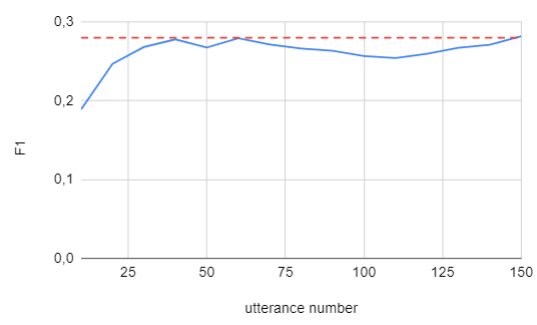
\includegraphics[0.5\textwidth]{imgs/increasing.PNG}
\vspace*{-0.3cm}
\end{adjustbox}
\caption{F1 when varying input length. The dotted red line shows the performance on the full input.}
\label{increasing}
\end{figure}

To investigate how many utterances are needed to make accurate predictions, we ran the trained PRIDE model on a subset of data with inputs of varying lengths.
To do so, we selected a subset of user pairs with at least 150 utterances, and perform inference while increasing the length of the slice of input utterances from 10 to 150.
This was repeated over 100 runs, with the randomized starting position of the slice.
The results averaged over all runs are shown in Figure \ref{increasing}.
We observe that approximately 40 utterances are enough to maximize performance in terms of F1 score.

\subsection{Per class analysis}

\begin{table}[]
\centering
\begin{adjustbox}{width=0.63\textwidth}
\begin{tabular}{@{}l|c|ccc@{}}
\textbf{class}      & \textbf{count} & \textbf{PRIDE} & \textbf{($-$ speaker)} & \textbf{($-$ dimensions)} \\ \toprule
friend                          & 208                             & 0.50                            & 0.50                                      & 0.50                 \\
lover                           & 187                             & 0.60                            & 0.58                                      & 0.60                 \\
spouse                          & 69                              & 0.40                            & 0.40                                      & 0.35                 \\
colleague                       & 67                              & 0.25                            & 0.25                                      & 0.25                 \\
child                           & 48                              & 0.60                            & 0.51                                      & 0.56                 \\
parent                          & 41                              & 0.62                            & 0.55                                      & 0.60                 \\
sibling                         & 37                              & 0.42                            & 0.33                                      & 0.40                  \\
employee                        & 34                              & 0.29                            & 0.23                                      & 0.26                 \\
boss                            & 29                              & 0.04                            & 0.08                                      & 0.04                 \\
enemy                           & 27                              & 0.14                            & 0.13                                      & 0.14                 \\
medical                         & 19                              & 0.46                            & 0.47                                      & 0.44                 \\
commercial                      & 19                              & 0.12                            & 0.12                                      & 0.06            
\end{tabular}
\end{adjustbox}
\caption{Class F1 scores of PRIDE and PRIDE without speaker embeddings and interpersonal dimensions.}
\label{perclass}
\end{table}

In Table \ref{perclass} we show the label distribution and per class F1 scores for PRIDE and two ablated versions.
We observe that using speaker embeddings benefit predictions on asymmetric classes, such as \emph{child} and \emph{parent}, as their F1 scores drop significantly when speaker embeddings are not used. Removing interpersonal dimensions damages performance on \textit{spouse} and \textit{child} in particular, illustrating  how this signal can help differentiate relationships that use similar vocabulary.


\subsection{Misclassification analysis}

\begin{figure}[t!]
\centering
\begin{adjustbox}{width=0.6\textwidth}
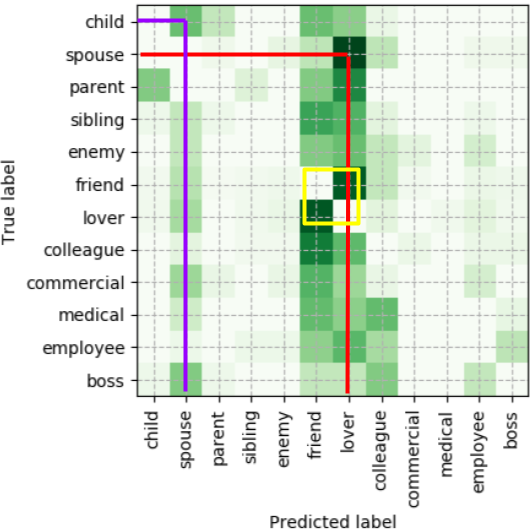
\includegraphics[0.3\textwidth]{imgs/confusion_marked.png}
\vspace*{-0.3cm}
\end{adjustbox}
\caption{Confusion matrix}
\label{confusion}
\end{figure}

The confusion matrix for PRIDE's predictions is shown in Figure \ref{confusion}. To create the confusion matrix for the multi-label case, we consider only incorrect predictions (either the labels which the model omitted or which it falsely predicted). For a single test instance we remove true positives from its sets of correct and predicted labels and use the Cartesian product of these sets to build the matrix.

We observe that there are many misclassifications into the \emph{friend} and \emph{lover} labels, which are the most common (see columns).
This can be attributed to the model's tendency to predict majority classes because of a considerable class imbalance. 

Considering specific pairs, we see that the model often confuses \emph{spouse} for \emph{lover} (red line). They may talk to each other in a similar tone and use the same address terms. Conceptually, however, these classes are different, with spouses having tighter family bonds, discussing children and household issues, and lovers talking more casually.
Similarly, \emph{child} and \emph{spouse} are often confused as well (purple line). Both may use terms related to family and discuss similar topics. The differences between \emph{lover} and \emph{friend} are indeed subtle (yellow square), and these pairs were also sometimes confused by human annotators.

Finally, we investigated the impact of confusion within asymmetric classes (for example, confusing \emph{parent} to \emph{child}). We found that if we accept the model's predictions of either label as correct, the average number of false positives for such classes drops by 34\%, resulting in an increase in average F1 score from 0.38 to 0.43.
This illustrates the challenge posed by considering relationship directions and the importance of including asymmetric labels.


\section{Conclusion}

We presented PRIDE, a model for inferring fine-grained relationships from conversations. To our best knowledge, PRIDE is the first model to predict \textit{directed, multilabel} speakers' relationships. PRIDE leverages the hierarchical dialogue structure to efficiently handle lengthy conversational history. The novelty of our architecture is the additional signals of speakers' demographics and speech style, which significantly improve relationship prediction.

PRIDE outperforms state-of-the-art baselines and demonstrates effective transfer learning on different types of dialogue data. %In ablation experiments we demonstrate that the proposed architecture improves the model's predictions. 
PRIDE is designed to perform inference on long conversational sequences; however, we experimentally show PRIDE's ability to make accurate predictions for shorter interactions too. 

To support future work on this topic, we created and released the largest labeled collection of relationships in conversations, which improves over existing datasets by including directed multilabel relationships.

\subsection{Discussion}

In this subsection we discuss several limitations of the current work and propose directions for further improvements of PRIDE:

\begin{itemize}
    \item \textbf{Leveraging other types of conversational data.} Inferring relationships in real-life user conversations is the use case motivating our research. Thus, we find it important to evaluate PRIDE's transfer learning capabilities to other conversational datasets to ensure that it can generalize. Our choice of the dataset was constrained by the complexity of labeling dialogues with relationship labels; we leave it for future work to obtain more diverse relationship datasets (for example, social media interactions or telephone transcripts).
    
    \item \textbf{Improving performance on directed relationships.} Predicting asymmetric relationships has been overlooked in the prior works; yet accurately distinguishing them is important for practical applications. For instance, an intelligent assistant can recommend completely different items, depending of whether the user is asking for a birthday present suggestions for her \textit{parent} or her \textit{child}. Thus, we find it necessary to further improve PRIDE's performance on asymmetric relationships.
    
    \item \textbf{Incorporating more personal attributes.} In our experiments we showed that prediction of interpersonal relationships can benefit from adding speakers' attributes. We find it interesting to experiment on adding other personal information, such as \textit{occupation} or \textit{ethnicity}.

    \item \textbf{Joint prediction of personal attributes and interpersonal relationships.} The current version of PRIDE supports incorporating precomputed ground truth information about the speakers' ages. In the scenario when personal attribute labels are not available, one option is to use a predictive model (such as HAM) to provide such information on the fly. Joint training of the relationship and speakers' attribute prediction models could improve their performance, as relationships and personal attributes are interdependent.

    \item \textbf{Considering multispeaker conversations.} The current dataset used in experiments with PRIDE was limited to uninterrupted dialogue spans between two characters. This limitation was due to the difficulty of distinguishing the addressee of an utterance when more than 2 speakers are present. In real life people often interact in a group, thus considering only speaker pairs will result in losing useful cues for predictions. Therefore, extension of the current model to handle multi-speaker conversations should be further investigated.
    %Therefore, we find it important to investigate the ways the current model can be extended to handle multi-speaker dialogues.

    
\end{itemize}

%The last research direction can also be generalized to the other models discussed in the current thesis. For instance, the people who communicate are often in the same age group and = have the same \textit{hobbies} (if they are friends) or \textit{professions} (if they are colleagues). We highlight simultaneous predictions of personal attributes and relationships using speaker network as a compelling future research direction.

\chapter{Conclusion}
\label{chap_conclusion}

\droppedcapital{T}{his} thesis is concerned with predicting personal knowledge from conversations. Such information can be used to populate a personal knowledge base, enhancing many downstream applications. The ambiguity of conversational utterances makes it challenging to automatically process them; thus the task of speakers' attribute inference is underexplored in related work. In our research we overcome the limitations of the prior studies, proposing the models which can accurately predict a wide range of personal facts.

%We explore inferring personal facts from dialogue data, which is abundant but challenging to automatically process.  Given the challenging nature of the conversational data, inferring speakers' attributes is particularly difficult and is currently underexplored in the related work. Yet, the knowledge of such attributes can augment many downstream applications. In our research we make a step towards creating models capable of predicting personal information.

In Chapter \ref{chap_ham} we described \textit{Hidden Attribute Models} (HAMs), capable of predicting speakers' demographic attributes: \textit{age}, \textit{gender}, \textit{profession} and \textit{family status}. HAMs utilize hierarchical conversational structure, making precise predictions at low computational costs. We have shown the capacity of HAMs to transfer learn among different conversational datasets, which is essential for applying the model to the real-life scenarios.

In Chapter \ref{chap_charm} we presented \textit{Conversational Hidden Attribute Retrieval Model} (CHARM), designed for predicting the values of the long-tailed \textit{profession} and \textit{hobby} attributes in a zero-shot setup. We propose a novel model design, which incorporates external knowledge to detect personal attribute values absent from the training data. CHARM makes predictions extracting keywords from the users' utterances, which ensure model's interpretability. 

In Chapter \ref{chap_pride} we introduced \textit{PRIDE}, a model for \textit{Predicting Relationships In Dialogue Excerpts}. Unlike most prior studies, PRIDE predicts fine-grained directed relationships, which are often ambiguous even for the human evaluators. We show that blending in additional signals, such as speakers' demographic attributes, can significantly improve interpersonal relationship inference.

Additionally, to support our experiments we issued several conversational datasets, described in Chapter \ref{chap_datasets}. Our datasets cover multiple personal attributes, based on the dialogues in the movies and interactions on social media, providing diverse inputs for the models. Our labeling strategies and manual verification ensure high precision of the provided data, which will be valuable for further research and practical applications.

\section{Future research directions}

The research in this dissertation is only an initial step for a comprehensive and accurate prediction of personal information from conversations. In this section we list possible directions for further investigations, which we find essential for building practical and user-friendly personalized systems.

\paragraph{Open-ended attributes.} Topical and user-oriented chat-bot recommendations require the knowledge of many open-ended personal attributes, e.g., \textit{favorite actor}. It is infeasible to enumerate all possible values for such attributes, especially given that new values constantly emerge. Predicting such facts might require dedicated unsupervised extraction methods.

\paragraph{Continuous incremental predictions.} An important aspect of conversational data is that the input utterances are spread in time, arriving as conversation proceeds. The utterances might contain contradictory cues, reflecting the change in the user's preferences (or even the user's demographics). Keeping an up-to-date state of the personal knowledge base as the conversation proceeds is an important issue, which can be addressed by learning personal facts from conversations incrementally.

\paragraph{Evaluating third party information.} All our proposed models make predictions about a speaker (or a speaker pair) based on their own utterances. However, a significant amount of information can be obtained by capturing the input from other conversation participants. Ideally, the model should be able to capture both the cues from subject's direct  interlocutor (``\textit{you must be coming from your shift at the hospital}'') and from a third person, when the subject is not even present in the current conversation (``\textit{Brandon is doing a lot of overtime in the hospital recently}''). 

\paragraph{Utilizing speaker network.} Building up on the previous point, we propose that the predictions of multiple personal attributes and relationships can be made simultaneously for a group of speakers, either within a current conversation or across multiple dialogues. A good example when such approach can facilitate predictions is utilizing the dependency of interpersonal relationships (from the fact that A and B are \textit{children} of C one can infer that A and B are \textit{siblings}). We envision that joint inference for all conversation participants can be performed with graph methods, which enable information sharing between the speakers (graph nodes).

\paragraph{Privacy issues.} Personal attributes is a sensitive information, the exposure of which can be harmful for the end user. Our proposed models supply the evidence for their predictions, which provides the pointers to disclosing content of the user. We propose more research to done into using this evidence to protect the users' personal data. 



%% Appendices
\cleardoublepage
\appendix

\backmatter

%% Bibliography
\cleardoublepage
\bibliography{bibliography}

\cleardoublepage
\listoffigures
\addcontentsline{toc}{chapter}{List of Figures}
\cleardoublepage
\listoftables
\addcontentsline{toc}{chapter}{List of Tables}

\printglossary[title=External Tools and Datasets, toctitle=External Tools and Datasets]

% \cleardoublepage
% \includepdf[pages=-, scale=1.0, addtotoc={1,chapter,1,Curriculum Vitae,mateusz_cv}]{mateusz_modern_cv/mateusz_CV}
% \addcontentsline{toc}{chapter}{Curriculum Vitae}

% \cleardoublepage
%\include{chapter-publications}
% \addcontentsline{toc}{chapter}{Selected Publications}

\end{document}
